%%%%%%%%%%%%%%%%%%%%%%%%%%%%%%%%%%%%%%%%%
% Classicthesis Typographic Thesis
% LaTeX Template
% Version 1.4 (1/1/16)
%
% This template has been downloaded from:
% http://www.LaTeXTemplates.com
%
% Original author:
% André Miede (http://www.miede.de) with commenting modifications by:
% Vel (vel@LaTeXTemplates.com)
%
% License:
% GNU General Public License (v2)
%
% General Tips:
% 1) Make sure to edit the classicthesis-config.file
% 2) New enumeration (A., B., C., etc in small caps): \begin{aenumerate} \end{aenumerate}
% 3) For margin notes: \marginpar or \graffito{}
% 4) Do not use bold fonts in this style, it is designed around them
% 5) Use tables as in the examples
% 6) See classicthesis-preamble.sty for useful commands
%
%%%%%%%%%%%%%%%%%%%%%%%%%%%%%%%%%%%%%%%%%

%----------------------------------------------------------------------------------------
%	PACKAGES AND OTHER DOCUMENT CONFIGURATIONS
%----------------------------------------------------------------------------------------

\documentclass[
		twoside,openright,titlepage,numbers=noenddot,headinclude,%1headlines,
	 	footinclude=true,cleardoublepage=empty,
		dottedtoc, % Make page numbers in the table of contents flushed right with dots leading to them
		BCOR=5mm,paper=a4,fontsize=11pt, % Binding correction, paper type and font size
		ngerman,american, % Languages, change this to your language(s)
		]{scrreprt} 
                
% Includes the file which contains all the document configurations and packages - make sure to edit this file
%%%%%%%%%%%%%%%%%%%%%%%%%%%%%%%%%%%%%%%%%
% Classicthesis Typographic Thesis
% Configuration File
%
% This file has been downloaded from:
% http://www.LaTeXTemplates.com
%
% Original author:
% André Miede (http://www.miede.de) with extensive commenting changes by:
% Vel (vel@LaTeXTemplates.com)
%
% License:
% GNU General Public License (v2)
%
% Important note:
% The main lines to change in this file are in the DOCUMENT VARIABLES
% section, the rest of the file is for advanced configuration.
%
%%%%%%%%%%%%%%%%%%%%%%%%%%%%%%%%%%%%%%%%%

%----------------------------------------------------------------------------------------
%	CHARACTER ENCODING
%----------------------------------------------------------------------------------------

\PassOptionsToPackage{utf8}{inputenc} % Set the encoding of your files. UTF-8 is the only sensible encoding nowadays. If you can't read äöüßáéçèê∂åëæƒÏ€ then change the encoding setting in your editor, not the line below. If your editor does not support utf8 use another editor!
\usepackage{inputenc}

%----------------------------------------------------------------------------------------
%	DOCUMENT VARIABLES
%	Fill in the lines below to enter your information into the thesis template
%	Each of the commands can be cited anywhere in the thesis
%----------------------------------------------------------------------------------------

% Remove drafting to get rid of the '[ Date - classicthesis version 4.0 ]' text at the bottom of every page
\PassOptionsToPackage{eulerchapternumbers,listings,drafting, pdfspacing, subfig,beramono,eulermath,parts}{classicthesis}
% Available options: drafting parts nochapters linedheaders eulerchapternumbers beramono eulermath pdfspacing minionprospacing tocaligned dottedtoc manychapters listings floatperchapter subfig

\newcommand{\myTitle}{A Classic Thesis Style\xspace}
\newcommand{\mySubtitle}{An Homage to The Elements of Typographic Style\xspace}
\newcommand{\myDegree}{Bachelor of Information Technology (Honours)\xspace}
\newcommand{\myName}{Yiping Su\xspace}
\newcommand{\myProf}{dfafa \xspace}
\newcommand{\myOtherProf}{Put name here\xspace}
\newcommand{\mySupervisor}{Cheng Soon Ong\xspace}
\newcommand{\myFaculty}{Put data here\xspace}
\newcommand{\myDepartment}{College of Engineering and Computer Science\xspace}
\newcommand{\myUni}{Australian National University\xspace}
\newcommand{\myLocation}{Canberra\xspace}
\newcommand{\myTime}{February 2020\xspace}
\newcommand{\myVersion}{version 0.2\xspace}

%----------------------------------------------------------------------------------------
%	USEFUL COMMANDS
%----------------------------------------------------------------------------------------

\newcommand{\ie}{i.\,e.}
\newcommand{\Ie}{I.\,e.}
\newcommand{\eg}{e.\,g.}
\newcommand{\Eg}{E.\,g.} 

\newcounter{dummy} % Necessary for correct hyperlinks (to index, bib, etc.)
\providecommand{\mLyX}{L\kern-.1667em\lower.25em\hbox{Y}\kern-.125emX\@}
\newlength{\abcd} % for ab..z string length calculation

%----------------------------------------------------------------------------------------
%	PACKAGES
%----------------------------------------------------------------------------------------

\usepackage{lipsum} % Used for inserting dummy 'Lorem ipsum' text into the template

%------------------------------------------------

%\PassOptionsToPackage{ngerman,american}{babel}  % Change this to your language(s)
% Spanish languages need extra options in order to work with this template
%\PassOptionsToPackage{spanish,es-lcroman}{babel}
\usepackage{babel}

%------------------------------------------------			

\usepackage{csquotes}
\PassOptionsToPackage{%
% backend=biber, % Instead of bibtex
backend=bibtex8,bibencoding=ascii,%
language=auto,%
style=numeric-comp,%
%style=authoryear-comp, % Author 1999, 2010
%bibstyle=authoryear,dashed=false, % dashed: substitute rep. author with ---
sorting=nyt, % name, year, title
maxbibnames=10, % default: 3, et al.
%backref=true,%
natbib=true % natbib compatibility mode (\citep and \citet still work)
}{biblatex}
\usepackage{biblatex}
 
 %------------------------------------------------

\PassOptionsToPackage{fleqn}{amsmath} % Math environments and more by the AMS 
 \usepackage{amsmath}

 %------------------------------------------------

\PassOptionsToPackage{T1}{fontenc} % T2A for cyrillics
\usepackage{fontenc}

%------------------------------------------------

\usepackage{textcomp} % Fix warning with missing font shapes

%------------------------------------------------

\usepackage{scrhack} % Fix warnings when using KOMA with listings package  

%------------------------------------------------

\usepackage{xspace} % To get the spacing after macros right

%------------------------------------------------

\usepackage{mparhack} % To get marginpar right

%------------------------------------------------

\usepackage{fixltx2e} % Fixes some LaTeX stuff 

%------------------------------------------------

\PassOptionsToPackage{smaller}{acronym} % Include printonlyused in the first bracket to only show acronyms used in the text
\usepackage{acronym} % Nice macros for handling all acronyms in the thesis

%\renewcommand*{\acsfont}[1]{\textssc{#1}} % For MinionPro
\renewcommand*{\aclabelfont}[1]{\acsfont{#1}}

%------------------------------------------------

\PassOptionsToPackage{pdftex}{graphicx}
\usepackage{graphicx} 

%----------------------------------------------------------------------------------------
%	FLOATS: TABLES, FIGURES AND CAPTIONS SETUP
%----------------------------------------------------------------------------------------

\usepackage{tabularx} % Better tables
\setlength{\extrarowheight}{3pt} % Increase table row height
\newcommand{\tableheadline}[1]{\multicolumn{1}{c}{\spacedlowsmallcaps{#1}}}
\newcommand{\myfloatalign}{\centering} % To be used with each float for alignment
\usepackage{caption}
\captionsetup{font=small}
\usepackage{subfig}  

%----------------------------------------------------------------------------------------
%	CODE LISTINGS SETUP
%----------------------------------------------------------------------------------------

\usepackage{listings} 
%\lstset{emph={trueIndex,root},emphstyle=\color{BlueViolet}}%\underbar} % For special keywords
\lstset{language=[LaTeX]Tex,%C++ % Specify the language(s) for listings here
morekeywords={PassOptionsToPackage,selectlanguage},
keywordstyle=\color{RoyalBlue}, % Add \bfseries for bold
basicstyle=\small\ttfamily, % Makes listings a smaller font size and a different font
%identifierstyle=\color{NavyBlue}, % Color of text inside brackets
commentstyle=\color{Green}\ttfamily, % Color of comments
stringstyle=\rmfamily, % Font type to use for strings
numbers=left, % Change left to none to remove line numbers
numberstyle=\scriptsize, % Font size of the line numbers
stepnumber=5, % Increment of line numbers
numbersep=8pt, % Distance of line numbers from code listing
showstringspaces=false, % Sets whether spaces in strings should appear underlined
breaklines=true, % Force the code to stay in the confines of the listing box
%frameround=ftff, % Uncomment for rounded frame
%frame=single, % Frame border - none/leftline/topline/bottomline/lines/single/shadowbox/L
belowcaptionskip=.75\baselineskip % Space after the "Listing #: Desciption" text and the listing box
}

%----------------------------------------------------------------------------------------
%	HYPERREFERENCES
%----------------------------------------------------------------------------------------

\PassOptionsToPackage{pdftex,hyperfootnotes=false,pdfpagelabels}{hyperref}
\usepackage{hyperref}  % backref linktocpage pagebackref
\pdfcompresslevel=9
\pdfadjustspacing=1

\hypersetup{
% Uncomment the line below to remove all links (to references, figures, tables, etc), useful for b/w printouts
%draft, 
colorlinks=true, linktocpage=true, pdfstartpage=3, pdfstartview=FitV,
% Uncomment the line below if you want to have black links (e.g. for printing black and white)
%colorlinks=false, linktocpage=false, pdfborder={0 0 0}, pdfstartpage=3, pdfstartview=FitV, 
breaklinks=true, pdfpagemode=UseNone, pageanchor=true, pdfpagemode=UseOutlines,%
plainpages=false, bookmarksnumbered, bookmarksopen=true, bookmarksopenlevel=1,%
hypertexnames=true, pdfhighlight=/O,%nesting=true,%frenchlinks,%
urlcolor=webbrown, linkcolor=RoyalBlue, citecolor=webgreen, %pagecolor=RoyalBlue,%
    %urlcolor=Black, linkcolor=Black, citecolor=Black, %pagecolor=Black,%
%------------------------------------------------
% PDF file meta-information
pdftitle={\myTitle},
pdfauthor={\textcopyright\ \myName, \myUni, \myFaculty},
pdfsubject={},
pdfkeywords={},
pdfcreator={pdfLaTeX},
pdfproducer={LaTeX with hyperref and classicthesis}
%------------------------------------------------
}

%----------------------------------------------------------------------------------------
%	AUTOREFERENCES SETUP
%	Redefines how references in text are prefaced for different 
%	languages (e.g. "Section 1.2" or "section 1.2")
%----------------------------------------------------------------------------------------

\makeatletter
\@ifpackageloaded{babel}
{
\addto\extrasamerican{
\renewcommand*{\figureautorefname}{Figure}
\renewcommand*{\tableautorefname}{Table}
\renewcommand*{\partautorefname}{Part}
\renewcommand*{\chapterautorefname}{Chapter}
\renewcommand*{\sectionautorefname}{Section}
\renewcommand*{\subsectionautorefname}{Section}
\renewcommand*{\subsubsectionautorefname}{Section}
}
\addto\extrasngerman{
\renewcommand*{\paragraphautorefname}{Absatz}
\renewcommand*{\subparagraphautorefname}{Unterabsatz}
\renewcommand*{\footnoteautorefname}{Fu\"snote}
\renewcommand*{\FancyVerbLineautorefname}{Zeile}
\renewcommand*{\theoremautorefname}{Theorem}
\renewcommand*{\appendixautorefname}{Anhang}
\renewcommand*{\equationautorefname}{Gleichung}
\renewcommand*{\itemautorefname}{Punkt}
}
\providecommand{\subfigureautorefname}{\figureautorefname} % Fix to getting autorefs for subfigures right
}{\relax}
\makeatother

%----------------------------------------------------------------------------------------

\usepackage{classicthesis} 

%----------------------------------------------------------------------------------------
%	CHANGING TEXT AREA 
%----------------------------------------------------------------------------------------

%\linespread{1.05} % a bit more for Palatino
% \areaset[current]{400pt}{761pt} % 686 (factor 2.2) + 33 head + 42 head \the\footskip
\setlength{\marginparwidth}{9em}%
% \setlength{\marginparsep}{2em}%

%----------------------------------------------------------------------------------------
%	USING DIFFERENT FONTS
%----------------------------------------------------------------------------------------

%\usepackage[oldstylenums]{kpfonts} % oldstyle notextcomp
%\usepackage[osf]{libertine}
%\usepackage[light,condensed,math]{iwona}
%\renewcommand{\sfdefault}{iwona}
%\usepackage{lmodern} % <-- no osf support :-(
%\usepackage{cfr-lm} % 
%\usepackage[urw-garamond]{mathdesign} <-- no osf support :-(
%\usepackage[default,osfigures]{opensans} % scale=0.95 
%\usepackage[sfdefault]{FiraSans}


% \usepackage[margin=1in]{geometry}
\usepackage{amssymb}
% \usepackage{amsmath}
\usepackage{bm}
% \usepackage{xcolor}

% \usepackage[english]{babel}
% \usepackage[utf8]{inputenc}
\usepackage{algorithm}
% \usepackage{algpseudocode}
% \usepackage{algorithmic}
\usepackage[noend]{algpseudocode}
\usepackage{enumitem}

\usepackage{float}
% \usepackage{graphicx} % Required for inserting images
% \usepackage{subcaption}

\graphicspath{{Figures/}{./}} 

\def\R{\mathrm I\!R}
\def\x{\bm{x}}
\DeclareMathOperator*{\argmax}{arg\,max}
\DeclareMathOperator*{\argmin}{arg\,min}

\renewcommand{\algorithmicrequire}{\textbf{Input:}}
\renewcommand{\algorithmicensure}{\textbf{Output:}}

\addbibresource{Bibliography.bib} % The file housing your bibliography
%\addbibresource[label=ownpubs]{Self_Publications.bib} % Uncomment for optional self-publications

%\hyphenation{Put special hyphenation here}

\begin{document}

\frenchspacing % Reduces space after periods to make text more compact

\raggedbottom % Makes all pages the height of the text on that page

\selectlanguage{american} % Select your default language - e.g. american or ngerman

%\renewcommand*{\bibname}{new name} % Uncomment to change the name of the bibliography
%\setbibpreamble{} % Uncomment to include a preamble to the bibliography - some text before the reference list starts

\pagenumbering{roman} % Roman page numbering prior to the start of the thesis content (i, ii, iii, etc)

\pagestyle{plain} % Suppress headers for the pre-content pages

%----------------------------------------------------------------------------------------
%	PRE-CONTENT THESIS PAGES
%----------------------------------------------------------------------------------------

% % Title Page

\begin{titlepage}

\begin{addmargin}[-1cm]{-3cm}
\begin{center}
\large

\hfill
\vfill

\begingroup
\color{Maroon}\spacedallcaps{Quantile estimation on streaming data} \\ \bigskip % Thesis title
\endgroup

\spacedlowsmallcaps{Yiping Su} % Your name

\vfill

\includegraphics[width=6cm]{gfx/TFZsuperellipse_bw} \\ \medskip % Picture

A study on something I don't quite understand yet \\ \medskip % Thesis subtitle
%\myDegree \\
%\myDepartment \\
%\myFaculty \\
%\myUni \\ \bigskip

February 2020 -- \myVersion % Time and version

\vfill

\end{center}
\end{addmargin}

\end{titlepage} % Main title page

% % Back of the title page

\thispagestyle{empty}

\hfill

\vfill

\noindent\myName: \textit{\myTitle,} \mySubtitle, %\myDegree, 
\textcopyright\ \myTime

% You may wish to do something with the back of the title page, such as including your supervisors, location or time frame of the work. Below is an example of doing so although you may want to tweak it to your liking.

%\bigskip

%\noindent\spacedlowsmallcaps{Supervisors}: \\
%\myProf \\
%\myOtherProf \\ 
%\mySupervisor

%\medskip \\

%\noindent\spacedlowsmallcaps{Location}: \\
%\myLocation

%\medskip \\

%\noindent\spacedlowsmallcaps{Time Frame}: \\
%\myTime
 % Back of the title page

% \cleardoublepage% Dedication

\thispagestyle{empty}
\refstepcounter{dummy}

\pdfbookmark[1]{Dedication}{Dedication} % Bookmark name visible in a PDF viewer

\vspace*{3cm}

\begin{center}
\emph{Ohana} means family. \\
Family means nobody gets left behind, or forgotten. \\ \medskip
--- Lilo \& Stitch    
\end{center}

\medskip

\begin{center}
Dedicated to the loving memory of Rudolf Miede. \\ \smallskip
1939\,--\,2005
\end{center} % Dedication page

%\cleardoublepage\include{FrontBackMatter/Foreword} % Uncomment and create a Foreword.tex to include a foreword

% \cleardoublepage% Abstract

%\renewcommand{\abstractname}{Abstract} % Uncomment to change the name of the abstract

\pdfbookmark[1]{Abstract}{Abstract} % Bookmark name visible in a PDF viewer

\begingroup
\let\clearpage\relax
\let\cleardoublepage\relax
\let\cleardoublepage\relax

\chapter*{Abstract}

Finding the quantiles of an unknown distribution is a good way of characterising the distribution, but for large amounts of streaming data, this is infeasible. Instead, methods for estimation of quantiles of streaming data have been developed for decades but are rarely related with the rapidly growing topic machine learning.
Stochastic gradient descent is a common machine learning method, which we apply in our quantile estimation algorithm SGD. This simple SGD algorithm is shown to be equivalent in some sense to the state-of-the-art Frugal-1U. 
In an effort to understand the convergence of SGD, we empirically compare the SGD performance under different settings of data distribution, data size, data ordering and SGD step size. Our experiments show that SGD is sensitive to the distribution and size of the data, as well as the step size.
As the only such parameter we can control, we propose two step size adaptation approaches, which improve the convergence rate of SGD on our test data.
Finally, we explore two algorithms for simultaneous estimation of multiple quantiles, and briefly discuss how their optimisations might be applied to our SGD algorithm.
Despite its simplicity, SGD converges to the true quantile with only O(1) space complexity, making it a very efficient quantile estimation algorithm.

\endgroup			

\vfill % Abstract page

% \cleardoublepage% Publications - a page listing research articles written using content in the thesis

\pdfbookmark[1]{Publications}{Publications} % Bookmark name visible in a PDF viewer

\chapter*{Publications} % Publications page text

Some ideas and figures have appeared previously in the following publications:\\

\noindent Put your publications from the thesis here. The packages \texttt{multibib} or \texttt{bibtopic} etc. can be used to handle multiple different bibliographies in your document.

%\begin{refsection}[ownpubs]
%    \small
%    \nocite{*} % is local to to the enclosing refsection
%    \printbibliography[heading=none]
%\end{refsection}

%\emph{Attention}: This requires a separate run of \texttt{bibtex} for your \texttt{refsection}, \eg, \texttt{ClassicThesis1-blx} for this file. You might also use \texttt{biber} as the backend for \texttt{biblatex}. See also \url{http://tex.stackexchange.com/questions/128196/problem-with-refsection}. % Publications from the thesis page

% \cleardoublepage% Acknowledgements

\pdfbookmark[1]{Acknowledgements}{Acknowledgements} % Bookmark name visible in a PDF viewer

\begin{flushright}{\slshape    
We have seen that computer programming is an art, \\ 
because it applies accumulated knowledge to the world, \\ 
because it requires skill and ingenuity, and especially \\
because it produces objects of beauty.} \\ \medskip
--- \defcitealias{knuth:1974}{Donald E. Knuth}\citetalias{knuth:1974} \citep{knuth:1974}
\end{flushright}

\bigskip

%----------------------------------------------------------------------------------------

\begingroup

\let\clearpage\relax
\let\cleardoublepage\relax
\let\cleardoublepage\relax

\chapter*{Acknowledgements}

\noindent Put your acknowledgements here.\\

\noindent Many thanks to everybody who already sent me a postcard!\\

\noindent Regarding the typography and other help, many thanks go to Marco Kuhlmann, Philipp Lehman, Lothar Schlesier, Jim Young, Lorenzo Pantieri and Enrico Gregorio\footnote{Members of GuIT (Gruppo Italiano Utilizzatori di \TeX\ e \LaTeX )}, J\"org Sommer, Joachim K\"ostler, Daniel Gottschlag, Denis Aydin, Paride Legovini, Steffen Prochnow, Nicolas Repp, Hinrich Harms, Roland Winkler, and the whole \LaTeX-community for support, ideas and some great software.

\bigskip

\noindent\emph{Regarding \mLyX}: The \mLyX\ port was initially done by
\emph{Nicholas Mariette} in March 2009 and continued by
\emph{Ivo Pletikosi\'c} in 2011. Thank you very much for your work and the contributions to the original style.

\endgroup % Acknowledgements page

\pagestyle{scrheadings} % Show chapter titles as headings

% \cleardoublepage% Table of Contents - List of Tables/Figures/Listings and Acronyms

\refstepcounter{dummy}

\pdfbookmark[1]{\contentsname}{tableofcontents} % Bookmark name visible in a PDF viewer

\setcounter{tocdepth}{2} % Depth of sections to include in the table of contents - currently up to subsections

\setcounter{secnumdepth}{3} % Depth of sections to number in the text itself - currently up to subsubsections

\manualmark
\markboth{\spacedlowsmallcaps{\contentsname}}{\spacedlowsmallcaps{\contentsname}}
\tableofcontents 
\automark[section]{chapter}
\renewcommand{\chaptermark}[1]{\markboth{\spacedlowsmallcaps{#1}}{\spacedlowsmallcaps{#1}}}
\renewcommand{\sectionmark}[1]{\markright{\thesection\enspace\spacedlowsmallcaps{#1}}}

\clearpage

\begingroup 
\let\clearpage\relax
\let\cleardoublepage\relax
\let\cleardoublepage\relax

%----------------------------------------------------------------------------------------
%	List of Figures
%----------------------------------------------------------------------------------------
    
% \refstepcounter{dummy}
% %\addcontentsline{toc}{chapter}{\listfigurename} % Uncomment if you would like the list of figures to appear in the table of contents
% \pdfbookmark[1]{\listfigurename}{lof} % Bookmark name visible in a PDF viewer

% \listoffigures

% \vspace{8ex}
% \newpage

%----------------------------------------------------------------------------------------
%	List of Tables
%----------------------------------------------------------------------------------------

% \refstepcounter{dummy}
% %\addcontentsline{toc}{chapter}{\listtablename} % Uncomment if you would like the list of tables to appear in the table of contents
% \pdfbookmark[1]{\listtablename}{lot} % Bookmark name visible in a PDF viewer

% \listoftables
        
% \vspace{8ex}
% \newpage
    
%----------------------------------------------------------------------------------------
%	List of Listings
%---------------------------------------------------------------------------------------- 

% \refstepcounter{dummy}
% %\addcontentsline{toc}{chapter}{\lstlistlistingname} % Uncomment if you would like the list of listings to appear in the table of contents
% \pdfbookmark[1]{\lstlistlistingname}{lol} % Bookmark name visible in a PDF viewer

% \lstlistoflistings 

% \vspace{8ex}
% \newpage
       
%----------------------------------------------------------------------------------------
%	Acronyms
%----------------------------------------------------------------------------------------

% \refstepcounter{dummy}
% %\addcontentsline{toc}{chapter}{Acronyms} % Uncomment if you would like the acronyms to appear in the table of contents
% \pdfbookmark[1]{Acronyms}{acronyms} % Bookmark name visible in a PDF viewer

% \markboth{\spacedlowsmallcaps{Acronyms}}{\spacedlowsmallcaps{Acronyms}}

% \chapter*{Acronyms}

% \begin{acronym}[UML]
% \acro{DRY}{Don't Repeat Yourself}
% \acro{API}{Application Programming Interface}
% \acro{UML}{Unified Modeling Language}
% \end{acronym}  
                   
\endgroup

 % Contents, list of figures/tables/listings and acronyms

% \cleardoublepage

\pagenumbering{arabic} % Arabic page numbering for thesis content (1, 2, 3, etc)
%\setcounter{page}{90} % Uncomment to manually start the page counter at an arbitrary value (for example if you wish to count the pre-content pages in the page count)

% \cleardoublepage % Avoids problems with pdfbookmark



% \ctparttext{You can put some informational part preamble text here. Illo principalmente su nos. Non message \emph{occidental} angloromanic da. Debitas effortio simplificate sia se, auxiliar summarios da que, se avantiate publicationes via. Pan in terra summarios, capital interlingua se que. Al via multo esser specimen, campo responder que da. Le usate medical addresses pro, europa origine sanctificate nos se.} % Text on the Part 1 page describing  the content in Part 1

% \part{Some Kind of Manual} % First part of the thesis

%----------------------------------------------------------------------------------------
%	THESIS CONTENT - CHAPTERS
%----------------------------------------------------------------------------------------
\chapter{Introduction and Background}
\label{ch: intro}

\graphicspath{{Figures/Intro/}{./}} 

In the situation when a large amount of data comes like a flow, data analysts might be interested in the how is the data distributed, or in other words, where are the densely and sparse parts of the distribution. For example, the managers of an online shopping system might be interested in the distribution of customers' age of an online sales event. As they want to find the majority of age groups for a more efficient advertisement, the question of the distribution is "what is the age diving points of the youngest 10\% and the oldest 10\%".  On one hand, the most updated distribution analysis is expected for a rapid adaptation, while on the other hand there is limited storage for the large amount of incoming data. In this paper, we explore this problem as a quantile estimation problem on data streams, and try to find space-efficient and computationally cheap solutions using the stochastic gradient descent method.

\section{Quantiles}
\label{sec: intro_quant}
Quantiles are the cutting points of a statistical distribution by its ranking. Specifically, the $\tau$-quantile is the cutting point that divides the distribution by probability $\tau$. Let $\tau$-q denote the $\tau$-quantile. For example, a $0.5$-q is the median of a distribution, such that there is a $50\%$ probability that a random sample is smaller than it. Generally, the value of a quantile can be achieved by mathematical approaches when the expression of the distribution is given. 
The quantiles are an important statistical feature of distributions for their values roughly reflects the density of the distribution.
For example, Fig \ref{fig: quant_example} shows samples from a Gaussian distribution and is annotated with two intervals [$0.5$-q, $0.9$-q] and [$0.9$-q, $0.99$-q]. The values of the intervals are similar, but the former contains 40\% data and the latter contains only 9\% data. Without any other information, this alone leads to the implication that the distribution is denser in the former interval than the latter.

\begin{figure*}[h!]
    \centering
	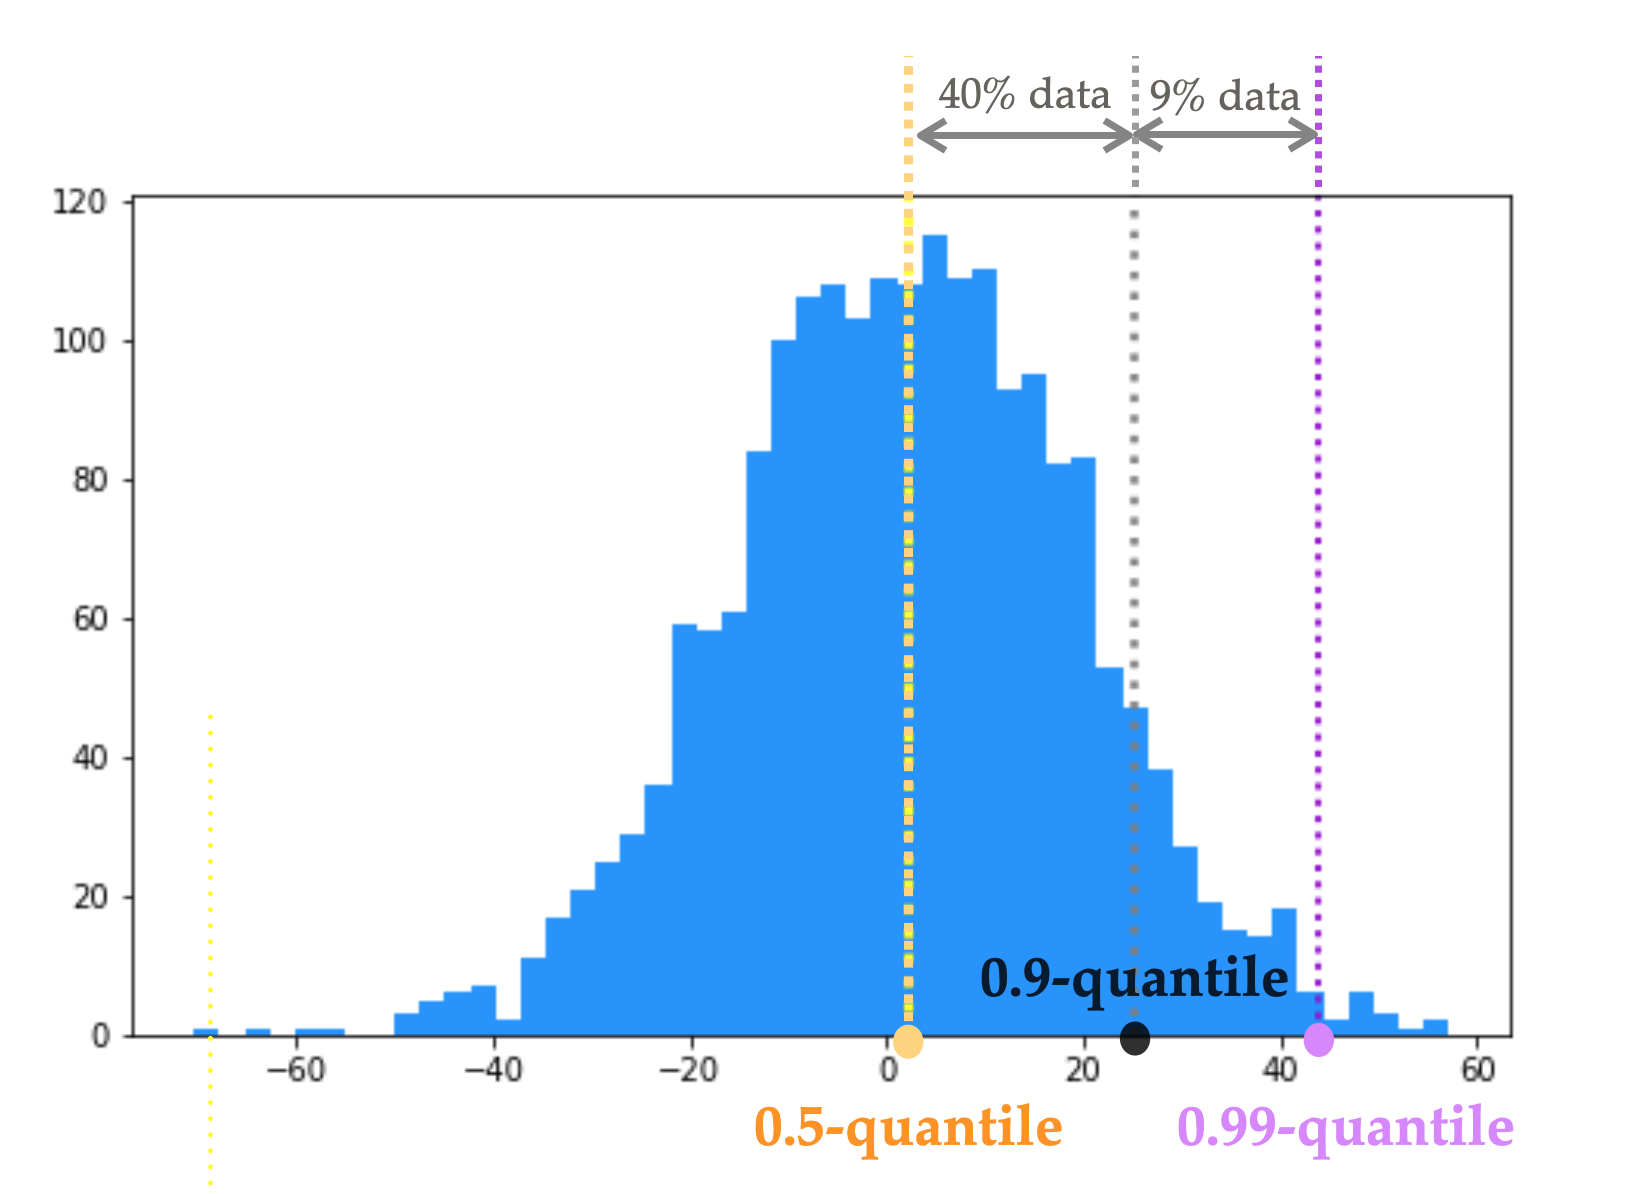
\includegraphics[width=0.6\columnwidth]{quant_example.png}
    \caption{Quantiles (0.5-q, 0.9-q and 0.99-q) of a dataset containing 2000 random samples from a Gaussian distribution (mean = 2, standard deviation = 18)}
    \label{fig: quant_example}
\end{figure*}

As shown in the example of Fig \ref{fig: quant_example}, the concept of quantiles are also applied in datasets as well as probability distributions. Similarly, the quantile for a finite dataset is the point which divides the dataset by probability $\tau$. However, since the dataset is discrete, the value of a $\tau$-q is ambiguous. For example, for dataset [$1,2,3,4$], both 2.01 and 2.99 can be considered as a valid value of $0.5$-q. Among various methods of dataset quantile estimations, we apply the one currently used by the \textit{Python 3} language. For a size $N$ dataset $X = \{x_1, ..., x_N\}$ , the method first finds the ranking index of the quantile $h = (N-1)\tau + 1$. If $h$ is not an integer, the estimated quantile is computed by linear interpolation between the two data points at ranking positions surround $h$
\begin{equation}
    \tau \text{-q}_{batch} = x_{\lfloor h\rfloor}+(h-\lfloor h\rfloor)\left(x_{\lfloor h\rfloor+1}-x_{\lfloor h\rfloor}\right)
\end{equation}
where $\lfloor h\rfloor$ is the greatest integer less than or equal to $h$. The computation result $\tau \text{-q}_{batch}$ is called a \textit{batch quantile}, since it comes from a batch of samples of a distribution.
\\\\
Note that although computing the quantiles of a sample estimates the quantiles of the associated distribution, this is not \"quantile estimation\" as it is referred to in this paper. Here the batch quantiles are regarded as computed quantiles, as a comparison of \textit{true quantiles} which are the real quantiles of the original probability distribution. The estimation of quantiles is introduced in the following part.

% Batch algorithm/True quantile: the naive sorting

\section{Data streams and quantile estimation}
\label{sec: intro_quant_est}

A \textit{Data stream} is a large source of data where data is created in sequence over a period of time. In contrast with datasets, data points are not instantly available all at a time, and that the size of the sample grows over time. Data streams are commonly seen in areas like network monitoring, data mining, financial trading systems, etc. Similarly to normal datasets, the value of quantiles is important for data analysis of data streams. Finding the quantiles of a data stream is the initial aim of this paper.

A trivial solution to find quantiles of data streams is to sort the entire data stream when the last data point arrives, and then compute the batch quantiles of the sorted dataset.  In cases when the size of the data stream is unknown, at the arrival of each data point, the batch quantiles are computed again so the quantile values get updated. The method of repeatedly sorting and computing batch quantiles is called the \textit{batch algorithm}. Due to the large size of the data streams, the batch algorithm for quantile computation is too expensive in both storage and computation to be a feasible solution for most computer systems.

Faced with the storage and computation problem, algorithms of \textit{quantile estimation} on data streams have been proposed. The quantile estimation algorithms do not store the entire data streams, and the algorithms return estimated quantiles that are close to the batch quantiles. Some quantile estimation algorithms are described in the literature review chapter. Although these algorithms use significantly less memory than the batch algorithm, most require a growing space complexity (i.e., correlated with size $N$). In this paper we investigate the space-efficient algorithms that use constant memory units for data streams of any size. Specifically, we focus on the machine learning method \textit{stochastic gradient descent} (SGD) for quantile estimation. 

\section{Stochastic gradient descent(SGD) for quantile estimation}
\label{sec: intro_GD_SGD}

\textit{Gradient descent} is a convex optimization algorithm that is commonly used in machine learning for loss function minimization. Gradient descent takes the entire dataset as the input, and by iteratively moving in the opposite direction of the gradient, it reaches the local minimum. Such method can also be used in quantile estimation if the entire dataset is available all at the same time.

\textit{Stochastic gradient descent (SGD)}, on the other hand, is the "online learning" version of gradient descent that updates iteratively when each new data point comes. For each data point, SGD steps in the opposite direction of the gradient computed from that data point. In this way, SGD updates using one data point at a time, rather than the whole dataset.
Fig \ref{fig: SGD_quant} shows how SGD is used to estimate quantiles on the same dataset of 2000 Gaussian distribution samples from Fig 1. It is shown in the figure that the SGD result fluctuates around the empirical quantile value, indicating SGD is a possible approach for quantile estimation.

\begin{figure*}[h!]
    % \centering
	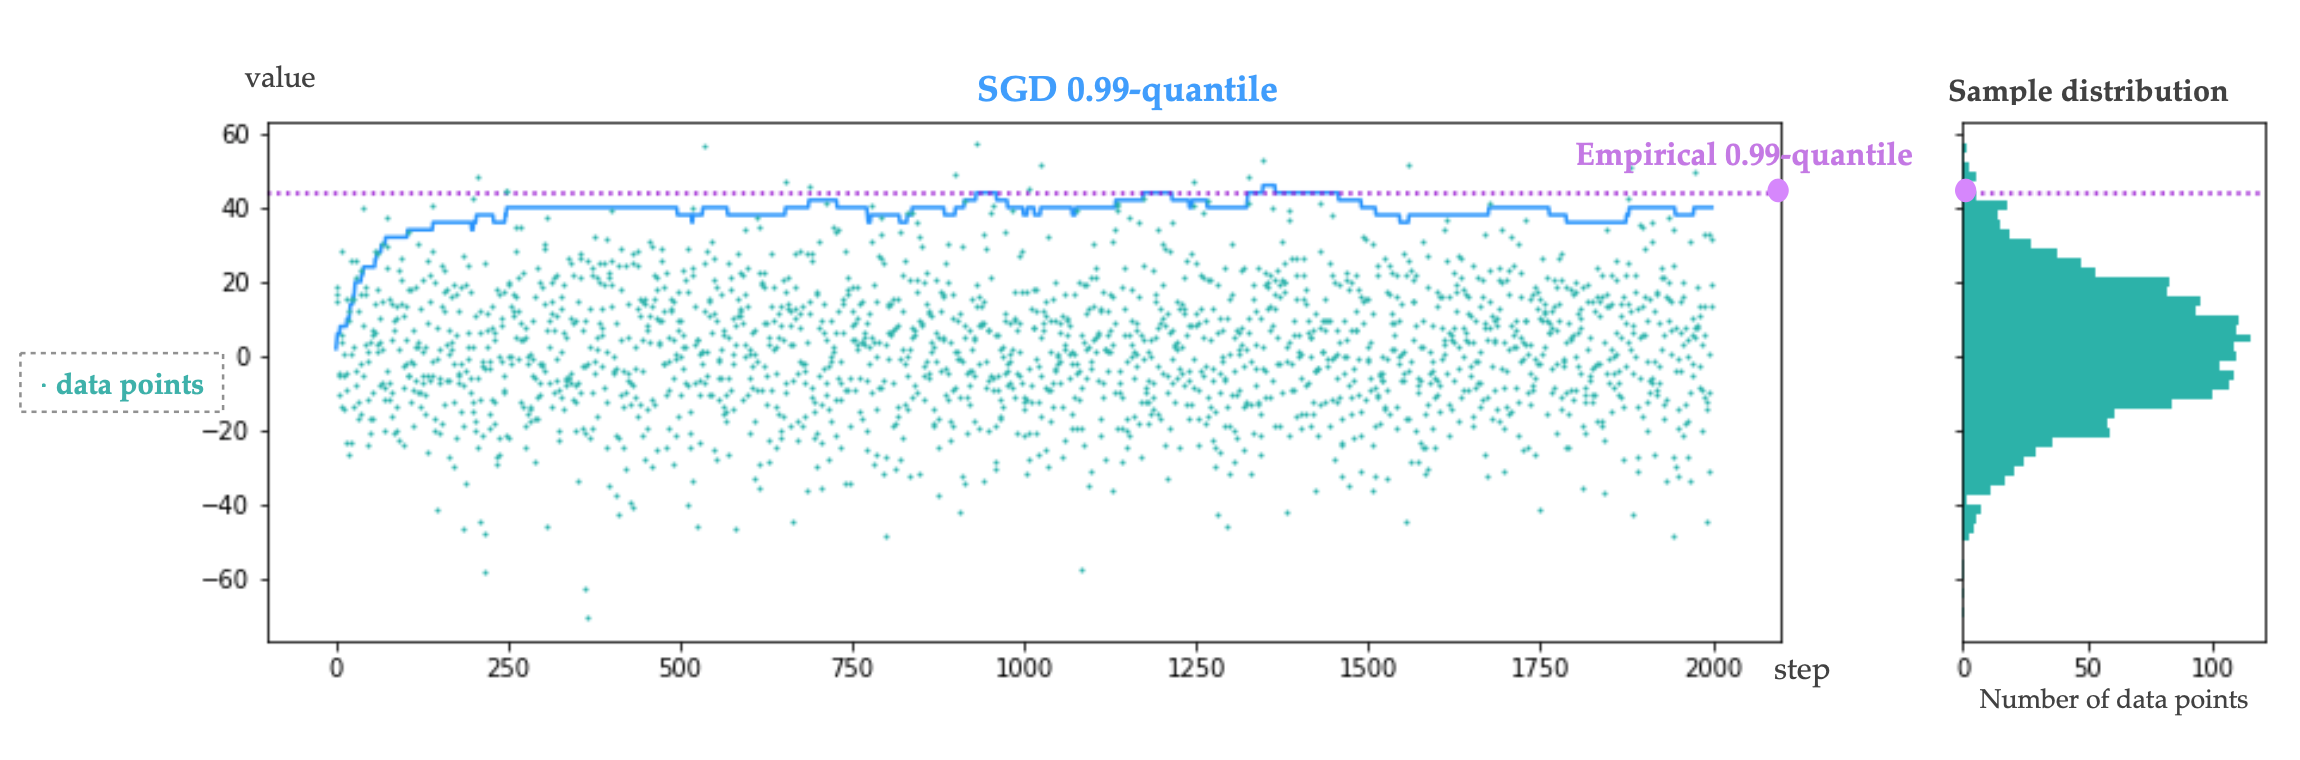
\includegraphics[width=1\columnwidth]{SGD_gaussian.png}
    \caption{SGD quantile estimation of the $0.99$-q for a dataset of 2000 samples from a Gaussian distribution. The left graph is a combination of incoming data points and the SGD steps, and each step of SGD is triggered by a new coming data point. The blue line shows how the SGD result is updated on the arrival of a data point (sea-green), and straight line (violet) represents the empirical value of $0.99$-q. On the right side, the density of the bell-shaped dataset is shown in a histogram.}
    \label{fig: SGD_quant}
\end{figure*}


\section{Background}

In this chapter, the essential background knowledge assumed throughout the rest of this thesis is defined. Subsection~\ref{subsec: sgd}introduces Stochastic Gradient Descent (SGD), which is a convex optimisation approach commonly found in machine learning, and subsection~\ref{subsec: quant} provides a definition for quantiles.
Stochastic gradient descent (SGD) is a convex optimization approach commonly applied in machine learning, and quantiles are the dividing points of a distribution or a dataset.

    \subsection{Gradient descent and stochastic gradient descent}
    \label{subsec: sgd}
    Stochastic gradient descent is an optimization algorithm developed from gradient descent. 
    \marginpar{References to be added here}
    Gradient descent was introduced by \textcolor{blue}{someone}, and is commonly used in \textcolor{blue}{something}

    \subsubsection{Gradient Descent}
        For convex optimization problems, gradient descent is a first-order optimization algorithm 
        to find the local minimum of a function.
        \\\\
        To solve the minimization problem 
        \begin{equation}
            % E
            \min_{\x} L(\x) 
        \end{equation} 
        
        where $L : \R^d \to \R$ is convex, differentiable and its gradient is Lipschitz continuous with constant
        $L > 0$.
        \\\\
        Geometrically, the gradient $\nabla L(\x_0)$ points to the direction of the steepest ascent on $L(\cdot)$ 
        from the point $\x_0$. 
        By taking a small step in the direction of the negative gradient, the function value is decreased in the 
        direction of the steepest descent. That is,
        \begin{equation}
            \x_1  = \x_0 - \alpha \nabla L(\x_0)
        \end{equation}
        for a small enough step size $\alpha \in \R_{+}$, then $L(\x_1) \leq L(\x_0)$. 
        That means, compared with $L(\x_0)$, $L(\x_1)$ is closer to the local minimum.
        \\\\
        With this observation comes the idea of gradient descent: an iterative "tour" on $L(\cdot)$ from a point towards the 
        local minimum by following small steps of negative gradient. 
        Let $\x_0$ be the guess of a starting point, then if
        % \marginpar{notation k should be i}
        \begin{equation}
            \x_{i+1} = \x_{i} - \alpha_i \nabla L(\x_i), i \geq 0
        \end{equation}
        
        
        Then we have $ L(\x_0) \geq L(\x_1) \geq L(\x_2) \geq \cdots$ where $\alpha_i$ is a suitable step size for iteration $i$. The convergence rate of the 
        sequence $(\x_n)$ with certain step size settings is linear in terms of the number of iterations.

        The objective function $L(\cdot)$ can be written as a sum of differentiable functions:%
        \begin{equation}
            L(\x) =\frac{1}{N} \sum_{n=1}^{N} \ell_n (\x)
        \end{equation}

        where the \textit{summand function} $\ell_n$ is usually the loss function of the $n$th observation among
        $N$ data points.
        \\\\
        Applying the gradient descent formula, $\x$ is updated according to%
        %
        \begin{equation}
           \x_{i+1} = \x_{i} -\alpha_i \nabla L(\x_i) = \x_{i} -\alpha_i \frac{1}{N}\sum_{n=1}^{N} \nabla \ell_n(\x_i) 
           \label{eq: background_gd_summand}
        \end{equation}

        From formula~\ref{eq: background_gd_summand}, it is clear that gradient descent requires access to all the data points to compute the movement direction, which is infeasible for a data stream.


    \subsubsection{Stochastic Gradient Descent (SGD)}
        Stochastic gradient descent was \textcolor{blue}{introduced by who because blabla, and commonly used bla}
        It is the choice for data streams, because the computation of the movement direction relies only on the most recent data point.
        It can be considered as a stochastic approximation of gradient descent optimization.
        \\\\
        The calculation of $\sum_{n=1}^{N} \nabla \ell_n(\x_i)$ can be
        expensive, especially when the amount of summand functions is huge, or when the individual gradients are hard to
        compute.
        To reduce the calculation, an estimation of the true gradient of $L(\x)$ is taken: 
        the true gradient $\frac{1}{N} \sum_{n=1}^{N} \nabla \ell_n(\x_i)$ is replaced by the gradient with respect to the $m$th observation, $\nabla \ell_m(\x_i)$. 
        So the update of the parameter $\x$ becomes%
        \begin{equation}
            \x_{i+1} = \x_i - \alpha_i \nabla \ell_m(\x_i)
        \end{equation}
        
        Generally, each time $m$ is randomly selected from $N$. In this paper, we use $m = i$ for quantile estimation on data streams.

\subsubsection{Limitations}
\marginpar{Not sure how I should mention this non-differentiable issue}
Since each SGD update requires only a single data point instead of the entire dataset, it becomes a great alternative for quantile estimation.
However, neither GD nor SGD can handle non-differentiable functions. This is an issue for the quantile estimation loss function in the following chapter.
Furthermore, while the computation per update is decreased $N$ times, the tradeoff lies in the convergence rate. SGD does not enjoy the same linear convergence rate as gradient descent. Both of these issues are discussed in chapter~\ref{ch: SAG}.


\subsection{Quantile}
\label{subsec: quant}

In statistics, quantiles are the points that divide a probability distribution into even intervals.
The $q$-quantiles ($q \in \{2,3,4,...\}$) is a set of quantile points which divides the distribution into $q$ intervals each with the same probability mass.
For example, the $2$-quantile has only one quantile point, which is the middle point of the distribution
and it divides the distribution into two even parts. This $2$-quantile point is called the median.
        \\\\
    \textbf{Definition with $q$-quantile notation} \\
    Generally, the $q$-quantiles have $q-1$ quantile points, and the $k$th quantile point for a 
    distribution $X$ is the data value such that%
    %
    \begin{equation}
        Pr(X \leq x) \geq \frac{k}{q}
    \end{equation}
    
    and%
    %
    \begin{equation}
        Pr(X \geq x) \geq 1 - \frac{k}{q}
    \end{equation}
    where $x \in X$.
    \\\\
    \textbf{Definition with notation $\tau$}\\
    Since $k < q$, we have $0 < \frac{k}{q} < 1$ for all ($k$,$q$) pairs. For $k, q \in \mathbb{N}^+$ we can define a quantile for any rational number in the interval $(0,1)$. For a quantile probability $\tau$, we use the notation $\tau$-quantile ($0 < \tau < 1$) for a quantile value in the distribution $X$ that satisfies%
    %
    \begin{equation}
        Pr(X \leq x) \geq \tau
    \end{equation}
    
    and%
    %
    \begin{equation}
        Pr(X \geq x) \geq 1 - \tau
    \end{equation}
    where $x \in X$.


\section{Thesis overview}
\label{sec: intro_overview}
In the final part of the introduction, we give a brief tour of the material in this paper.
The main focus of the paper is to explore how stochastic gradient descent method can be used for quantile estimation on data streams.
In chapter \ref{ch: literature_review}, a very brief discussion of quantile estimation algorithms is presented, with a special mention for space-efficient algorithms (e.g., SGD-like methods). 
Chapter \ref{ch: algo_equal} compares the SGD methods with the \textit{Frugal1U} algorithm\cite{maFrugalStreamingEstimating2014}, showing how the two similar methods are "equivalent" to some extent.
Chapter \ref{ch: sgd_exp} which presents experiments to illustrate the relationship between setting for SGD and its performance.
Next, chapter \ref{ch: SAG} and \ref{ch: multi_quant} explore the two extensions of the vanilla SGD algorithm: the step size adaptation of SGD and the simultaneous multi-quantile estimation. Finally, the work of the paper is summed up in the conclusion chapter \ref{ch: conclusion}.
\\\\
Fig \ref{fig: structure} is the layout of the contents of the paper.

\begin{figure*}[h!]
    \centering
	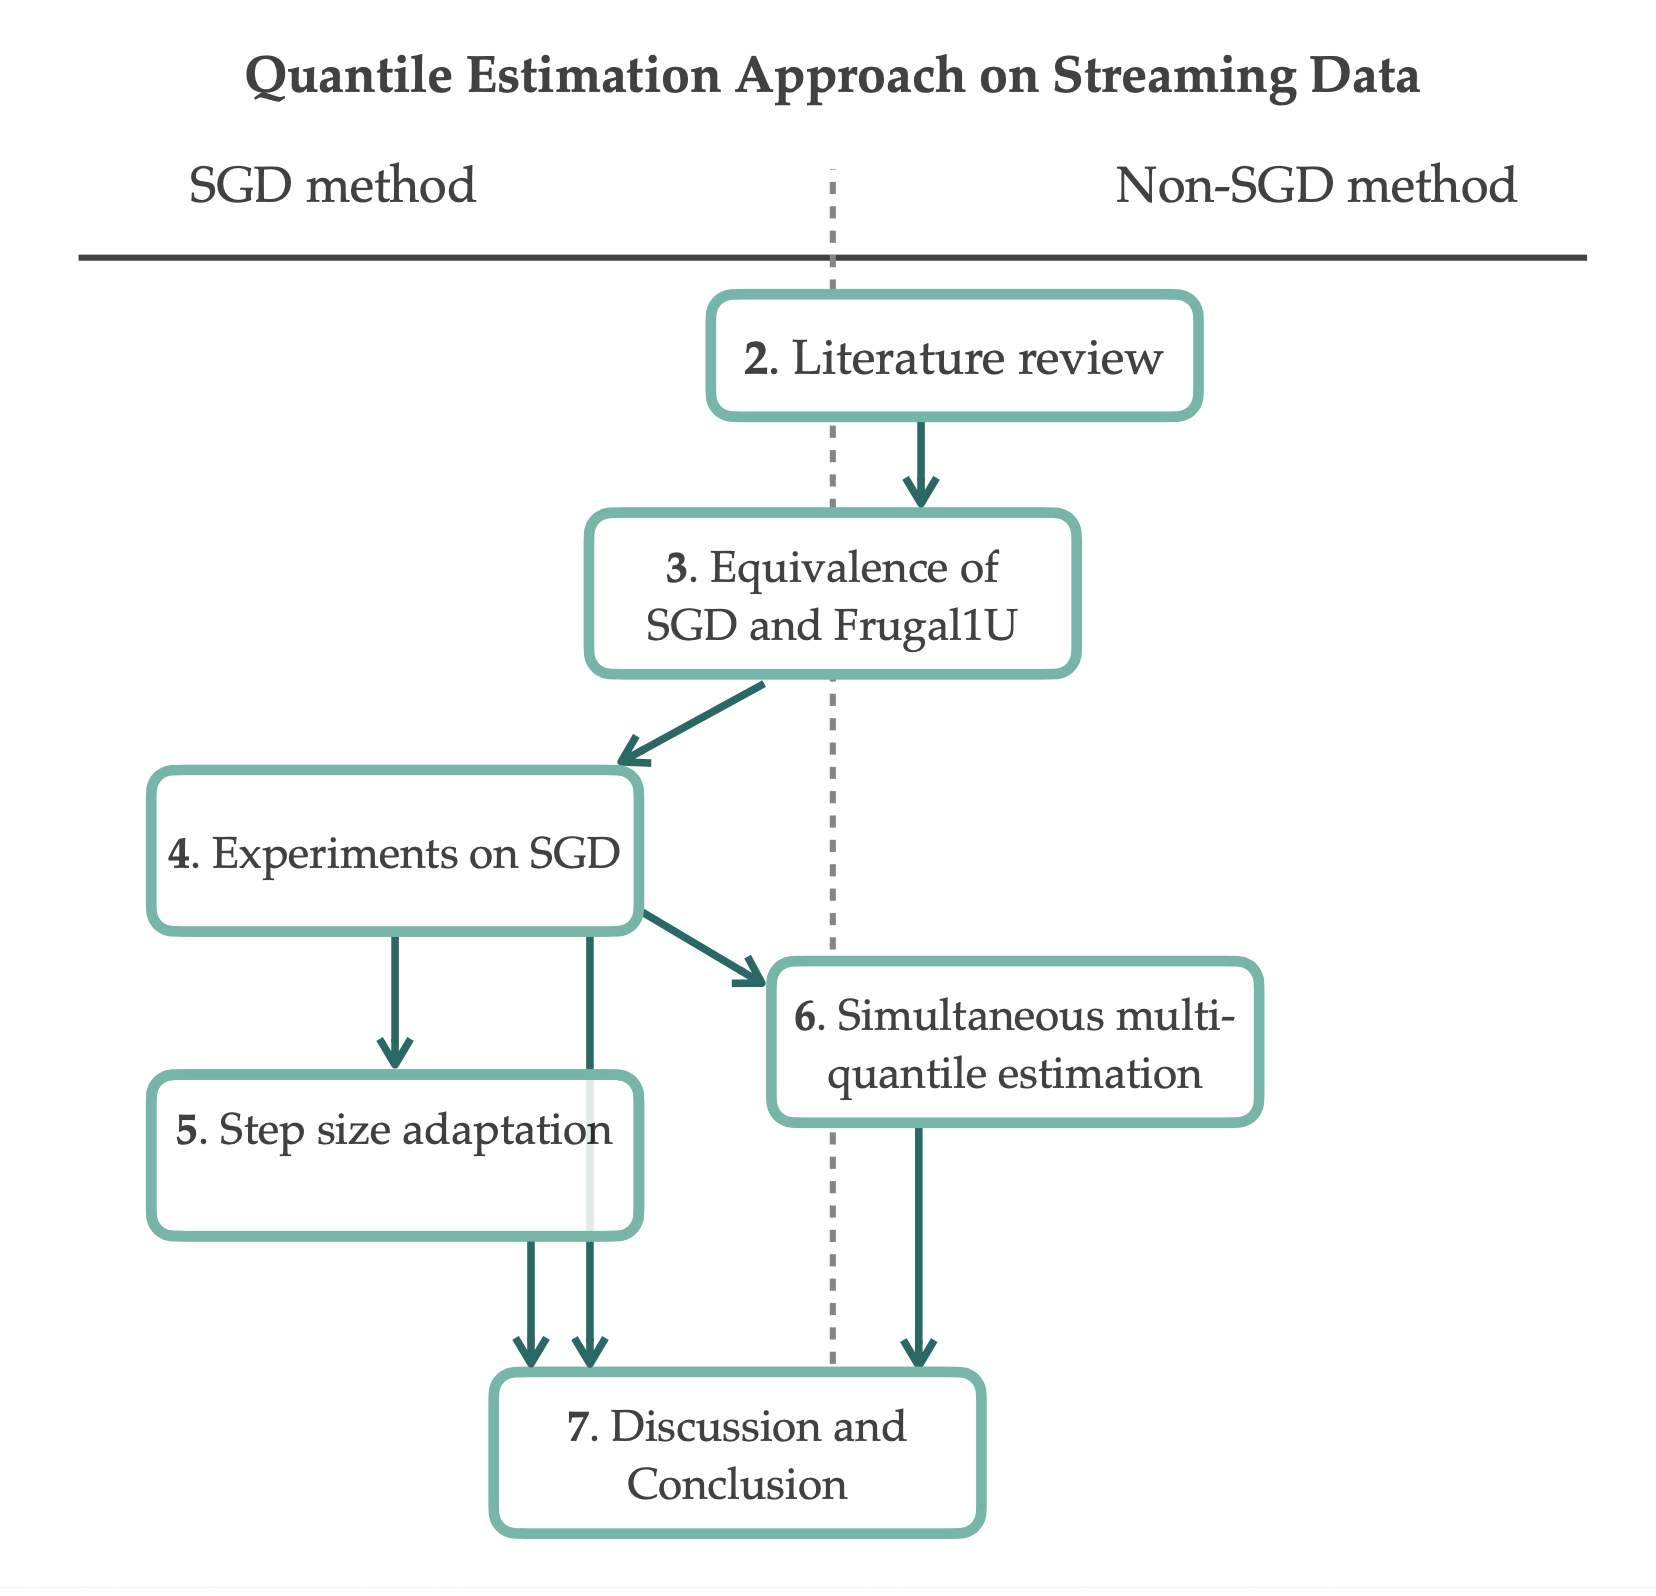
\includegraphics[width=0.8\columnwidth]{structure.png}
    \caption{The relationship between topics covered in the thesis. Topics are roughly positioned along the top-bottom axis depending on where they are more close to SGD methods (left) or non-SGD methods (right). The arrows between the chapters represent are connected according to dependence.}
    \label{fig: structure}
\end{figure*}

\marginpar{My contributions to be added here}
% \documentclass[12pt]{article}
\usepackage{xcolor}
\usepackage[margin=1in]{geometry}
\usepackage{amssymb}
\usepackage{amsmath}
\usepackage{bm}
\usepackage{xcolor}

\usepackage[english]{babel}
\usepackage[utf8]{inputenc}
\usepackage{algorithm}
% \usepackage{algpseudocode}
% \usepackage{algorithmic}
\usepackage[noend]{algpseudocode}
\usepackage{enumitem}


\def\R{\rm I\!R}
\def\x{\bm{x}}
\DeclareMathOperator*{\argmax}{arg\,max}
\DeclareMathOperator*{\argmin}{arg\,min}

\renewcommand{\algorithmicrequire}{\textbf{Input:}}
\renewcommand{\algorithmicensure}{\textbf{Output:}}

\title{Literature review outline}
\date{\vspace{-5ex}}


\begin{document}
\maketitle

\section{SGD 
            \color{blue}{(should it be in Background instread?)}}
    



\section{Quantile Estimation From Streaming Data}
\begin{enumerate}
    \item Why useful: \\
        \cite{rayArtApproximatingDistributions1800}(Industrial use) "
        Many businesses care about accurately computing quantiles over their key metrics, which can pose several interesting challenges at scale. 

        e.g. Price for advertisement on bidding level: quantile estimation helps price setting
        "\\\\
        Other industrial usage mentioned in \cite{hongEstimatingQuantileSensitivities2009}, and its citations for industrial use \\
        "
        Quantiles have been adopted by many industries as major
        measures of random performance. In the financial industry,
        quantiles, also known as value-at-risks (VaRs), are widely
        accepted measures of capital adequacy. For example, the
        Bank for International Settlement uses the 10-day VaR at
        the 99\% level to measure the adequacy of bank capital
        (Duffie and Pan 1997). In the service industry, quantiles
        are often used as measures of service quality. For example, the service quality of an out-of-hospital system is frequently measured by the 90th percentile of the times taken
        to respond to emergency requests and to transport patients
        to a hospital (Austin and Schull 2003). Quantiles have
        also been used as billing measures in some circumstances.
        For example, some Internet service providers (ISPs) charge
        their users based on the 95th percentile of the traffic load
        in a billing cycle (Goldenberg et al. 2004).
        "
    \item Pinball loss on quantile regression: \\
        \cite{steinwartEstimatingConditionalQuantiles2011}\\
        \cite{koenkerRegressionQuantiles1978}
    \item Simultaneously predicting several quantiles: \\
        \cite{sangnierJointQuantileRegression} (non-streaming)(multi-dimensional)(quantile regression)\\
    \item Quantile Streaming: \\
        \cite{greenwaldQuantilesEquidepthHistograms2016}\\
        \cite{maFrugalStreamingEstimating2014}\\
    \item Parallel Quantile Estimation from Streaming Data ((3) + (4)): \\
        \cite{jainP2AlgorithmDynamic1985}\\
        \cite{ben-haimStreamingParallelDecision}\\
        \cite{pebayFormulasRobustOnepass2008}\\

\end{enumerate}


\section{Anomaly Detection and Outlier}

\begin{enumerate}
    \item Anomaly detection: \\
        \cite{emmottMetaAnalysisAnomalyDetection2015}
        (industrial use)
        ()
        % \cite{huangOnlineAnomalousTime2013}
\end{enumerate}
\newpage
\textbf{My work} Quantile estimation on streaming data, which would be applied on 

\newpage
\bibliography{Thesis}
\bibliographystyle{ieeetr}

\end{document}
\end(documentclass) % Chapter 1
% % \documentclass[11pt]{article}

\chapter{Stochastic Gradient Descent}
\label{ch: sgd}
% \begin{document}
% \maketitle

\section{Stochastic Gradient Descent}

    Stochastic gradient descent (often abbreviated SGD) is an optimization algorithm developed from gradient descent. 
    In this section, gradient descent is introduced as the first part of the explanation of SGD.

    \subsection{Gradient Descent}
        For convex optimization problems, gradient descent is a first-order optimization algorithm 
        to find the local minimum of a function.
        \\\\
        To solve the minimization problem 
        \begin{equation}
            % E
            \min_{\x} L(\x) 
        \end{equation} 
        
        where $L : \R^d \to \R$ is convex, differentiable and its gradient is Lipschitz continuous with constant
        $L > 0$.
        \\\\
        Geometrically, the gradient $\nabla L(\x_0)$ points to the direction of the steepest ascent on $L(\cdot)$ 
        from the point $\x_0$. 
        By taking a small step in the direction of the negative gradient, the function value is decreased in the 
        direction of the steepest descent. That is,
        \begin{equation}
            \x_1  = \x_0 - \alpha \nabla L(\x_0)
        \end{equation}
    
        for a small enough stepsize $\alpha \in \R_{+}$, then $L(\x_1) \leq L(\x_0)$. 
        That means, compared with $L(\x_0)$, $L(\x_1)$ is closer to the local minimum.
        \\\\
        With this observation comes the idea of gradient descent: an iterative "tour" on $L(\cdot)$ from a point towards the 
        local minimum by following small steps of negative gradient. 
        Let $\x_0$ be the guess of a starting point, then if
        \begin{equation}
            \x_{k+1} = \x_{k} - \alpha_k \nabla L(\x_k), k \geq 0
        \end{equation}
        
        
        Then we have $ L(\x_0) \geq L(\x_1) \geq L(\x_2) \geq \cdots$ with suitable $\alpha_k$. The convergence of the 
        sequence $(\x_n)$ to the local minimum is guaranteed{\color{red} [reference]}.


    \subsection{Stochastic Gradient Descent}
        SGD can be considered as a stohcastic appoximation of gradient descent optimization, 
        when the objective function $L(\cdot)$ can be written as a sum of differentiable functions.
        Consider the objective function is in the form:
        \begin{equation}
            L(\x) =\frac{1}{K} \sum_{k=1}^{K} L_k (\x)
        \end{equation}

        where the summand function $L_k$ is usually the loss function of the $k$th observation among
        $K$ data points.
        \\\\
        Then by following the idea of gradient descent, the $\x$ is updated according to
        
        \begin{equation}
           \x_{k+1} = \x_{k} -\alpha_k \nabla L(\x_k) = \x_{k} -\alpha_k \frac{1}{K}\sum_{k=1}^{K} \nabla L_k(\x_k) 
        \end{equation}
        
        
        where each $\alpha_k$ is a suitable stepsize. The calculation of $\sum_{k=1}^{K} \nabla L_k(\x_k)$ can be
        expensive, especially when the amount of summand functions is huge, or when the individual gradients are hard to
        compute. 
        \\\\
        To reduce the consumption of calculation, an estimation of the true gradient of $L(\x)$ is taken: 
        the true gradient $\frac{1}{K} \sum_{k=1}^{K} \nabla L_k(\x_k)$ is replaced by the gradient of a single observation $\nabla L_k(\x_k)$. 
        So the update of the parameter $\x$ becomes
        
        \begin{equation}
            \x_{k+1} = \x_{k} - \alpha_k \nabla L_k(\x_k)
        \end{equation}
        
        where $\alpha_k$ is a suitable stepsize. 
        \\\\
        The convergence of SGD has been proved as well{\color{red} [reference]}. 
        \\\\\\
        (and should I explain more about why stochastic gradient descent works?)

% \documentclass[11pt]{article}

\usepackage[margin=1in]{geometry}
\usepackage{amssymb}
\usepackage{amsmath}
\usepackage{bm}
\usepackage{xcolor}

\usepackage[english]{babel}
\usepackage[utf8]{inputenc}
\usepackage{algorithm}
% \usepackage{algpseudocode}
% \usepackage{algorithmic}
\usepackage[noend]{algpseudocode}
\usepackage{enumitem}


\def\R{\rm I\!R}
\def\x{\bm{x}}
\DeclareMathOperator*{\argmax}{arg\,max}
\DeclareMathOperator*{\argmin}{arg\,min}

\renewcommand{\algorithmicrequire}{\textbf{Input:}}
\renewcommand{\algorithmicensure}{\textbf{Output:}}

\title{Proof of Algorithm Equivalence}
\author{Yiping Su}
\begin{document}
\maketitle
% --------------------------------------------------------------------------------
%                                Quantile Estimation
% --------------------------------------------------------------------------------
            
\section{Quantile Estimation}

\subsection{Quantile}

In statistics, quantiles are the points that divide a probability distribution into even intervals.
The $q$-quantiles devide the distribution into $q$ intervals each with the same amount of data points.
And there are $q$ quantile points of the $q-$quantiles.
For example, the $2$-quantile has only one quantile point, which is the middle point of the distribution
and it divides the distribution into two even parts. This $2$-quantile point is called the median.


\subsubsection{Definition} \label{tau-quantile-def}
Generally, the $q$-quantiles have $q-1$ quantile points, and the $k$th $q$-quantile for a 
distribution $X$ is the data value such that
$$
Pr(X \leq x) \geq \frac{k}{q}
$$
and
$$
Pr(X \geq x) \geq 1 - \frac{k}{q}
$$
where $x \in X$

\subsection{Quantile Estimation and Pinball Loss}
In this paper, the estimation for $\tau$-quantile 
($\tau =  \frac{1}{q}, \frac{2}{q}, \cdots, \frac{q-1}{q}$)
is applied.
Pinball loss function is one of the approaches for the estimation for a statistical population.
\\\\
For a one-dimentional data set $X = \{x_1, x_2, \cdots, x_N\}$, 
now consider the loss function for a single data point $x$ $(i \in {1, \cdots, N})$.
Let $t := x - q$ be the difference between the real value $x$ and the estimate of quantile $q$.
$l_{\tau}(\cdot): \R \to \R_{\geq 0}$ is the loss function on $t$ such that
$$
l_\tau(t)= 
    \begin{cases}
        \tau t & t > 0\\
        -(1-\tau) t & otherwise
    \end{cases}
$$
And the $\tau$-quantile loss has the {\color{red} subgradient}:
$$
\frac {\partial l_\tau(t)}{\partial t}= 
    \begin{cases}
        \tau                & t > 0\\
        -(1-\tau)           & t < 0\\
        [\tau, -(1 - \tau)] & t = 0
    \end{cases}
$$

The overall loss for distribution $X$ with quantile estimation $q$ is
$$
L_{\tau}(q) = \sum_{x \in X} l_{\tau}(x - q)
$$
The best estimate of the $\tau$-quantile $q$ is the $q$ with minimal overall loss. 
Let $q^\ast$ be the best estimate, then we have
$$
q^\ast = \argmin_{q} L_{\tau}(q)
$$


% --------------------------------------------------------------------------------
%                                SGD for Quantile Estimation
% --------------------------------------------------------------------------------
\section{Algorithm Equivalence}

\subsection{Pseudo Code for the Frugal-1U Algorithm}

Qiang Ma, S. Muthukrishnan and Mark Sandler {\color{red} [ref]}  
introduced the following algorithm \ref{alg:frugal_1U} which 
"uses only one unit of memory per group to compute a quantile for each group"({\color{blue} quotation}).

\begin{algorithm}
\caption{Frugal-1U}\label{alg:frugal_1U}
    \begin{algorithmic}[1]
        \Require{Data Stream $S$, $h$, $k$, $1$ unit of memory $\tilde{m}$}
        \Ensure{$\tilde{m}$}
        % \Procedure{frugal}{$X,\tau$}            \Comment{X is the dataset}
        \State {Initialization $\tilde{m} = 0$}               %\Comment{Default initialization $q_0$ = 0}
            \For{\textbf{each} $s_i$ in $S$}                  %\Comment{Parameter update for each input data point}
                \State{$rand$ = random(0,1); //get a random value in $[0,1]$}
                % \State {\textbf{set} $\alpha_k$} \Comment{Set stepsize}
                \If{$s_i > \tilde{m}$ \textbf{and} $rand > 1-\frac{h}{k}$} %\Comment{$q_{k+1} = q_k + \alpha_k \tau$ when $x_k - q_k > 0$}
                    \State{$\tilde{m} = \tilde{m} + 1$;}
                \Else { \textbf{if} $s_i < \tilde{m}$ \textbf{and} $rand > \frac{h}{k}$}  %\Comment{$q_{k+1} = q_k - \alpha_k (1-\tau)$ otherwise}
                    \State{$\tilde{m} = \tilde{m} - 1$;}
                \EndIf
            \State{\textbf{end if}}
            \EndFor
        \State{\textbf{end for}}
        % \State \textbf{return} $q$              \Comment{$q_k$ is the SGD result of quantile estimate}
        % \EndProcedure
    \end{algorithmic}
\end{algorithm}
The output $\tilde{m}$ is the estimate of the $h$th $k$-quantile for a given data stream $S$. 
By rephrasing of some steps of Frugal-1U, 
its equilalence to an SGD algorithm for quantile estimation will be shown in the follwing part.
\\\\
\textbf{Rephrasing of the Algorithm} \label{replacements}
\begin{enumerate}
    \item The constant $\frac{h}{k}$ is replaced by $\tau$, since the $\tau$-quantile is defined
     as the $h$th $k$-quantile point in section \ref{tau-quantile-def}.
    % \item The quantile estimate $\tilde{m}$ is replaced by $q$, as it stands for estimate of quantile.
    \item The generation of random number and it's comparison with $1-\frac{h}{k}$ or $\frac{h}{k}$
    in line 3 to 7 is replaced by the following algorithm.
    \begin{algorithm}
        \begin{algorithmic}[1]
            \setcounter{ALG@line}{2}
            \State{ }   \Comment{No need to generate a random number}
            \If{$s_i > \tilde{m}$} %\Comment{$q_{k+1} = q_k + \alpha_k \tau$ when $x_k - q_k > 0$}
                \State{$\tilde{m} = \tilde{m} + 1 \times (1-\frac{h}{k})$}     
                \Comment{$P((rand > 1-\frac{h}{k}) \mid rand \in \mathcal{U}(0,1)) = 1-\frac{h}{k}$;}
            \Else { \textbf{if} $s_i < \tilde{m}$}  %\Comment{$q_{k+1} = q_k - \alpha_k (1-\tau)$ otherwise}
                \State{$\tilde{m} = \tilde{m} - 1 \times \frac{h}{k}$}         
                \Comment{$P((rand > \frac{h}{k}) \mid rand \in \mathcal{U}(0,1)) = \frac{h}{k}$;}
            \EndIf 
        \end{algorithmic}
    \end{algorithm}

    % Here the probability $P((rand > p) \mid rand \in \mathcal{U}(0,1))$ is the simplification
    % for the generation of random number $rand$ and it's comparison to a constant $p$ $(0 < p < 1)$.
    
    To understand this replacement, let's consider the serie of the 3 steps: 
    (i) generate a random number $rand$, 
    (ii) compare it with a constant $p$, and
    (iii) take action if $rand > p$. 
    It can be interpreted as take the action with probability 
    $P((rand > p) \mid rand \in \mathcal{U}(0,1))$. 

    Mathmatically, the replacement works because the expected change of
    $\tilde{m}$ in both methods are the same. 
    For example when $s_i > \tilde{m}$, 
    the expected change of $\tilde{m}$ is
    $E_1[\nabla \tilde{m}] = E[\tilde{m} \times p]$ in the Frugal-1U with 
    random number generation,
    while 
    $E_2[\nabla \tilde{m}] = \tilde{m} \times p$ in the replacement method.
    Since $E_1[\nabla \tilde{m}] = E_2[\nabla \tilde{m}]$, the replacement is valid
    with regard to the expectation of the change in quantile estimate during each step.

\end{enumerate}


\subsection{SGD for Loss function}

Let $q_0$ be the initial guess of quantile estimate. 
By SGD, the estimate is updated each step with a data point from the distribution.
$$
q_{k+1} = q_k - \alpha_k g_k
$$
where $ \alpha_k $ is a suitable stepsize and 
$$
g_k = \partial L_{\tau}^{(k)}(q_k) \in \frac{\partial l_\tau(x_k - q_k)}{\partial q_k}
$$ 
\textbf{Notice: partial is taken because the gradient of a single variable function
euqals the partial of it}
\\\\
Then we have
$$
q_{k+1} = 
    \begin{cases}
        q_k + \alpha_k \tau               & x_k - q_k > 0\\
        q_k - \alpha_k (1-\tau)           & x_k - q_k \leq 0\\
        % [\tau, -(1 - \tau)] & t = 0
    \end{cases}
$$

\begin{algorithm}
    \caption{SGD algorithm}\label{alg:SGD}
    \begin{algorithmic}[1]
        \Require{Data Stream $X$, $\tau$, $1$ unit of memory $q$}
        \Ensure{$q$}
        % \Procedure{frugal}{$X,\tau$}            \Comment{X is the dataset}
        \State {Initialize} $q$                 \Comment{Default initialization $q_0$ = 0}
            \For{$x_k$ in $X$}                  \Comment{Parameter update for each input data point}
                \State \textbf{set} $\alpha_k$  \Comment{Set stepsize}
                \If{$x_k > q$}                  \Comment{$q_{k+1} = q_k + \alpha_k \tau$ when $x_k - q_k > 0$}
                    \State{$q = q + \alpha_k \tau$}
                \Else                           \Comment{$q_{k+1} = q_k - \alpha_k (1-\tau)$ otherwise}
                    \State{$q = q - \alpha_k (1-\tau)$}
                \EndIf
            \EndFor
        \State \textbf{return} $q$              \Comment{$q_k$ is the SGD result of quantile estimate}
        % \EndProcedure
    \end{algorithmic}
\end{algorithm}
% --------------------------------------------------------------------------------
%                              Equality of two algorithms 
% --------------------------------------------------------------------------------
\section{Equivalence of Algorithms}
In this section we'll show the equilalence of algorithm Frugal-1U 
and SGD.
\\\\
Besides the replacements mentioned in section \ref{replacements},
the notations have changed: 
$X$ is applied for the data stream, and $q$ instead of $\tilde{m}$
to represent quantile estimate.
The introduction of changable stepsize $\alpha_k$ for each data point $x_k$
is the highlight of the SGD algorithm. The flexibility of stepsize can help
with achieving a better convergence rate when stepsizes are chosen wisely.
Specifically, the setpsize is not mentioned in Frugal-1U 
because it is fixed as $1$. In SGD the stepsize might change for every step.

{\color{red} \textbf{Problem}}
In Frugal-1U the quantile estimate $q$ does not change when $x_k > q$, but in SGD 
the quantile estimate is updated: $q = q-\alpha_k (1-\tau)$. This can be seen as different 
\textbf{subgradient} values for $l_\tau(x_k - q_k)$ 
{\color{red} \textbf{but then I need to explain subgradient descent}} 


\end{document}


% \documentclass[12pt]{article}
\usepackage{xcolor}
\usepackage[nointegrals]{wasysym}

\usepackage[margin=1in]{geometry}
\usepackage{amssymb}
\usepackage{amsmath}
\usepackage{bm}
\usepackage{xcolor}

\usepackage[english]{babel}
\usepackage[utf8]{inputenc}
\usepackage{algorithm}
% \usepackage{algpseudocode}
% \usepackage{algorithmic}
\usepackage[noend]{algpseudocode}
\usepackage{enumitem}


\def\R{\rm I\!R}
\def\x{\bm{x}}
\DeclareMathOperator*{\argmax}{arg\,max}
\DeclareMathOperator*{\argmin}{arg\,min}

\renewcommand{\algorithmicrequire}{\textbf{Input:}}
\renewcommand{\algorithmicensure}{\textbf{Output:}}

\title{SGD Quantile Estimation Experiement}
\date{\vspace{-5ex}}

\begin{document}
\maketitle

\section{Introduction}

% \subsection你说“我就不该这么想”{Aims}
This experiment has two purposes. The first is to show quantile estimation with SGD works \textcolor{blue}{ under some circimstances (?)}.
The second aim is to investigate how different settings of the problem effect the estimation performance. Specifically, we are interested in the following aspects: data distribution, data size, data ordering, quantile value and sgd step size.
In the experiment, multiple ordered datasets are generated as input data streams, based on which the calculated and estimated quantile values are computed. Results of both quantiles are compared after processing. We want to compare the performance of quantile estimation over different settings.
\\\\
\textcolor{blue}{This experiment also aims at the comparison between Frugal algorithm and SGD algorithm, by which we want to show that those two algorithms are ``equivalent". 
\\
(Does it mean SGD estimation works?)}
% To test the SGD quantile estimation as a valid alternative for quantile estimation, this experiment computes both estimated and calculated values for quantiles, and evaluates whether the difference between the results is acceptable.
% \\\\
% Do I explain the second goal...?


\section{Methodology}
The process by which we experiment on SGD quantile estimation can be briefly outlined as followes:

\begin{enumerate}
    \item Select a set of data streams (ordered datasets) derived from some statistical distributions.
    \item For each $\tau$-quantile, determine a ground truth value from the distribution and calculate a empirical value from the data stream.
    \item For each $\tau$-quantile, calculate the SGD estimate value from the data stream, record both the process and the result of estimation.
    \item \textcolor{blue}{
        Compare Frugal algorithm and SGD algorithm on data streams of the same setting.
    }
    \item Compute normalized error value for quantile estimates as a measurement of similarity between empirical and estimate value. The error value is computed from both values.
\end{enumerate}

\subsection{Data Stream Set Generation}
A total of 4 distributions are used in this experiment.
Eah data stream is a set of 1 dimensional data points randomly sampled from one of the distributions. In order to show how the amount of data points might affect the performance, there are 3 different settings for the data size $N$. 
\\\\
Each data stream set is composed of a number of data streams. For a statistically more accurate results on the experiment, a group of data streams of the same settings are generated. When investigating the impact of data sequence has on quantile estimation, one data stream will be shuffled to for the generation to differently ordered data steams. To sum up, a data stream set is either a combination of data streams generated from same distribution and data size setting, or the permutations of one same data stream. We generate the data stream set under this settings:

\begin{itemize}
    \item Distribution: 4 statistical distributions. The 4 distributions are:
        \begin{itemize}
            \item Gaussian distribution 1: mean = 2, standard deviation = 18
            \item Gaussian distribution 2: mean = 0, standard deviation = 0.001
            \item Exponetial distribution: rate = 1
            \item Mixed Gaussian distribution: a mix of five different gaussian distributions
        \end{itemize}
    \item Data size: 100, 1000, 10000, 100000(?)
    \item Multiple generations: True or false. Generate 10 data streams for the set if true.
    \item Multiple shuffles:  True or false. Shuffle the data stream 10 times for the set if true.
\end{itemize}

\subsection{True and Empirical Quantile Calculation}
The true quantile values are the quantile values for the distributions which the data streams are derived from. They are calculated by the maths functions for quantile computation. All except the mixed gaussian distribution has a relatively easy function for quantile calculation. For the mixed distribution, the empirical quantile value from a large amount of sampling is taken for the true value. By this means, the empirical value is expected to be close enough to the true quantile value such that the evaluation of results is not much affected \textcolor{blue}{(needs more justification?)}. In this experiment, a total of 100,000,000 samples are generated for the calculation. For a certain $\tau$, there is only one true quantile value for one distribution.
\\\\
The empirical quantile value is the quantile value calculated from the data steam instead of the distribution. For a certain $\tau$, no matter what the ordering is, there is only one empirical quantile value for one data stream, but there can be multiple quantile values for one distribution.

\subsection{SGD Quantile Estimation}

The parameter of SGD quantile estimation is important. The current step sizes are:
\begin{itemize}
    \item Constant number: 1
    \item Decrease when k increases: 
    \item Decrease when k increases (smaller size):
\end{itemize}

\subsection{Frugal and SGD algorithm}

Frugal algorithm is proposed for quantile estimation as well. In this experiment, we want to compare the two algorithms and show they have similar performance for same data streams. In this experiment, data streams are generated from all 4 distributions, and the step size for SGD quantile estimation is set to constant 1.

\subsection{Error Computation}

In order to measure the performance of quantile estimation, the error measurement is proposed. At first, the error $E = | q_{batch} - q_{sgd} |$ is to show 

\section{Observations}


\section{Discussion? Accuracy of study?}
% \begin{equation}
%     E = | \frac{q_{batch} - q_{sgd}}{{q_{batch}}^{(1)} - {q_{batch}}^{(2)}} |
% \end{equation}
\section{Conclusion}

\end{document}
\end(documentclass)
% \chapter{Step Size Adaptation}
\label{ch: stepsize_adaptation}

\graphicspath{{Figures/Stepsize_adapt/}{./}} 

\section{Failure on Newton's Method}
\label{sec: newton}
Newton's method is an iterative method to find the stationary points (where the function's derivative is zero) of a twice-differentiable function $f$. The application of Newton's method failed for our SGD quantile methods, since the loss function of the quantile estimation function is not twice-differentiable. For a specific $\tau$, and $t := x - q$ be the difference between the input data value $x$ and the estimate of quantile $q$, the loss function 

\begin{equation}
    \ell_\tau(t)= 
        \begin{cases}
            \tau t & t > 0\\
            -(1-\tau) t & otherwise
        \end{cases}
\end{equation}


is a linear function of $t$, which doesn't have any second derivative. 
\\\\
Though the method cannot be applied, it is easy to reach the goal of Newton's method: to find the critical points of a function. Instead of stationary point, the loss function has a critical point where it is not differentiable and the derivative changes sign. For any $\tau \in (0,1)$, when $t=0$, the loss function reaches it's critical points at $\ell_\tau(0) = 0$. Taking the critical point for every step, however, does not contribute to any improvement in quantile estimation. To be at a critical point, the quantile estimate is set to have the equal value of input data $x$, and only in this way we could have $t = x-q = x-x = 0$. Regardless of $\tau$, the quantile estimate is always equal to the value of the latest data point. So far this method has totally failed its goal to estimate a quantile value based on $\tau$ and the entire data stream.
\\\\
From another perspective, the failure of Newton's method is the result of applying large step size for the last input data for a SGD method. In this way, the minimal of current loss function $\ell_\tau(t)$ is reached, while the total loss function for the input data stream $X$

\begin{equation}
    L_{\tau}(t) = \sum_{x \in X} \ell_{\tau}(t)
\end{equation}

is entirely ignored.

% ------------------------------------------------

\graphicspath{{Figures/Smooth_func/}{./}} 


\section{Stochastic Average Gradient (SAG)}
\label{sec: sag}
One approach on step size adaptation is to use the stochastic average gradient (SAG)\cite{schmidtMinimizingFiniteSums2016} algorithm. It is an convex optimization method that has a significant improvement of convergence rate than stochastic gradient (SG) methods. In general, the convergence rate is improved from $O(1/\sqrt{k})$ to $O(1/k)$ for a total of $k$ epochs, reaching the same level as the gradient descent method. Along with the rising convergence rate, it keeps a low computational cost for each iteration to be independent from the size of function sum.

\subsection{Mechanism of SAG}
Similar to SG methods, SAG methods aim for minimization of the sum of a finite number of smooth convex functions where $N$ is very large. The problem setting is
\begin{equation}
\underset{x \in \mathbb{R}^p}{\text{minimize}} g(x) := \frac{1}{N}\sum^N_{n=1} \ell_n(x)
\end{equation}
where each $\ell_n$ is a smooth convex function.

The standard (full) gradient (FG) method has each iteration in the form
\begin{equation}
x_{i+1} = x_i - \alpha_i g^{\prime} (x_i) = x_i - \frac{\alpha_i}{N}\sum^N_{n=1} \ell_n^{\prime}(x_i)
\end{equation}
where $\alpha_i$ is the step size of iteration $i$. For each iteration, the computational cost is $O(N)$.

To save the iteration cost, the stochastic gradient (SG) method has each iteration in the form
\begin{equation}
x_{i+1} = x_i - \alpha_i \ell_{m_i}^{\prime} (x_i)
\end{equation}
where $m_i$ is the index for the iteration that gets sampled from the range {$1, 2,...,n$}. It has an iteration cost of $O(1)$, but a much lower convergence rate.

The stochastic average gradient (SAG) remembers the last update of a gradient value for each index $i$, which enables the improvement of convergence rate from SG methods. Its iteration takes the form
\begin{equation}
x_{i+1} = x_i - \frac{\alpha_i}{N} \sum^N_{n=1}y_{m}^{i}
\end{equation}
where $y_{m}^{i}$ is used to keep the memory of recently updated gradient value of function $\ell_m$
\begin{equation}
y_{m}^{i}:=\left\{\begin{array}{ll}
    \ell_{m}^{\prime}\left(x_{i}\right) & \text { if } m=m_{i} \\
    y_{m}^{i-1} & \text { otherwise }
    \end{array}\right.
\end{equation}
The SAG algorithm, according to \citeauthor{schmidtMinimizingFiniteSums2016}, "like the FG method, the step incorporates a gradient with respect to each function". Meanwhile only one gradient computation is involved in the combination of gradients, such that the iteration cost is independent of $N$.

\subsubsection{Convergence guarantee}

Under the assumption that each $\ell_m$ is convex and the gradient $\ell_m\prime$ is \textit{Lipschitz continuous} with constant $L$, which means
\begin{equation}
|\ell_m\prime (a) - \ell_m\prime (b)| \leq L|a-b|
\end{equation}
for all $a,b \in \mathbb{R}^p$.
The SAG algorithm with constant step size $\alpha_i = \frac{1}{16L}$ reaches the convergence rate of $O(1/i)$. The convergence function differs when the $y_m^0$ is initialized differently, or when $l_m$ is strongly convex.


\subsection{Basic SAG algorithm}

\begin{algorithm}
    \caption{Basic SAG method for minimizing $\frac{1}{N} \sum^N_{n=1}\ell_n(x)$ with step size $\alpha$}\label{alg:SAG_ori}
        \begin{algorithmic}[1]
            \Require{Dataset $X$, Dataset Size $N$, Step size $\alpha$}
            \Ensure{$x$}
            % \Procedure{frugal}{$X,\tau$}            \Comment{X is the dataset}
            \State {$d = 0, y_m = 0$ for $m = 1, 2, ..., N$}           \Comment{Default initialization}
            \For{$i = 0,1,...$}                  %\Comment{Parameter update for each input data point}
                \State {Sample $m$ from $\{1,2,...,N\}$}
                \State {$d=d - y_m + \ell^{\prime}_m(x)$}
                \State {$y_m = \ell^{\prime}_m(x)$}                    \Comment{Save the $y_m$ in the table for re-visit}
                \State{$x = x - \frac{\alpha}{N}d$}
            \EndFor
            \State{\textbf{end for}}
        \end{algorithmic}
\end{algorithm}

The Basic SAG algorithm requires memory storage of a table of $y_m (m= 1, 2, ...,N)$, to keep the track of each $y_m$ in case they are re-visited after first update.

\subsection{SAG Implementation for quantile estimation}

The quantile estimation loss function is a convex function, and \textbf{we can use a smooth function for replacement}
\begin{algorithm}
    \caption{Basic SAG method for streaming data $S$ for quantile estimation}\label{alg:SAG}
        \begin{algorithmic}[1]
            \Require{Data Stream $X$, Data Stream Size $N$, $\tau$, $\tau$-quantile estimate $\tilde{q}$, Step size $\alpha$}
            \Ensure{$\tilde{q}$}
            % \Procedure{frugal}{$X,\tau$}            \Comment{X is the dataset}
            \State {Initialization $d = 0, \tilde{q}=0$}           \Comment{Default initialization $q_0=0$, $d_0=0$}
            \For{\textbf{each} $x_i$ in $X$}                  %\Comment{Parameter update for each input data point}
                \State {$d=d - 0 + \ell^{\prime}_{\tau}(x_i, \tilde{q})$} \Comment{$0$ stands for $y_m^{i-1}$}
                % \State {\textbf{set} $\alpha_k$} \Comment{Set stepsize}
                \State{$\tilde{q} = \tilde{q} - \frac{\alpha}{N}d$}
            \EndFor
            \State{\textbf{end for}}
        \end{algorithmic}
\end{algorithm}
For streaming data, it's worthwhile noticing that each input data point has exactly one pass. It means for the SAG implementation, the storage of updated $y_m^i$ is useless since it would not be revisited. Besides, if all $y_m^0$ are initialized as 0, the storage of $y^0$ initialization needs only one unit of memory instead of $N$ units of memory. in this way, we can keep the memory complexity of SAG quantile estimation to $O(1)$.

\subsection{Experiments on SAG}

In this section, we explore how SAG

\graphicspath{{Figures/Stepsize_adapt/SAG/}{./}} 

\begin{figure}[H]
    \centering
	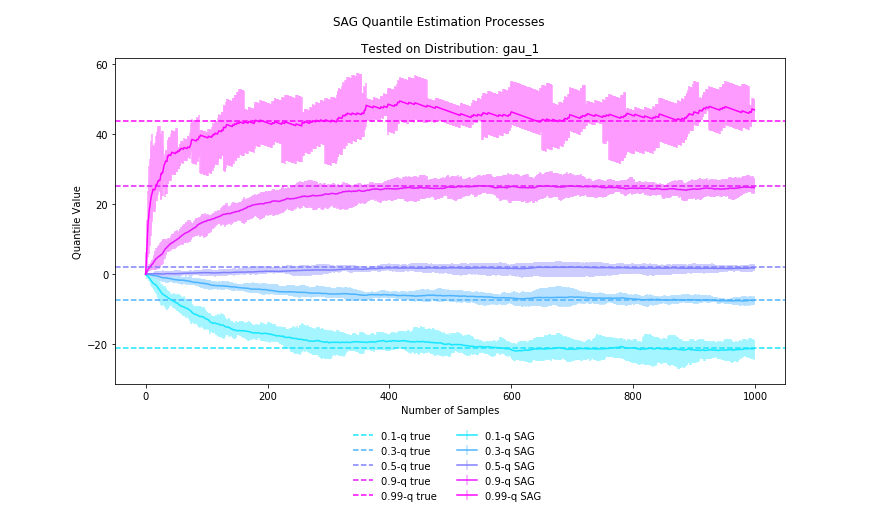
\includegraphics[width=1\columnwidth]{distro/gau_1_proc.png}
	\caption{SAG Process from \textit{gau-1} Distribution}
\end{figure}

\begin{figure}[H]
    \centering
	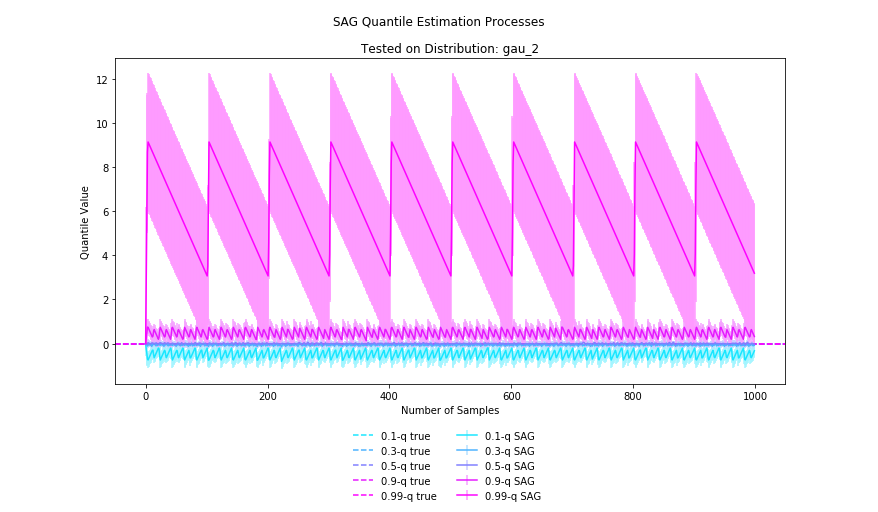
\includegraphics[width=1\columnwidth]{distro/gau_2_proc.png}
	\caption{SAG Process from  \textit{gau-2} Distribution}
\end{figure}

\begin{figure}[H]
    \centering
	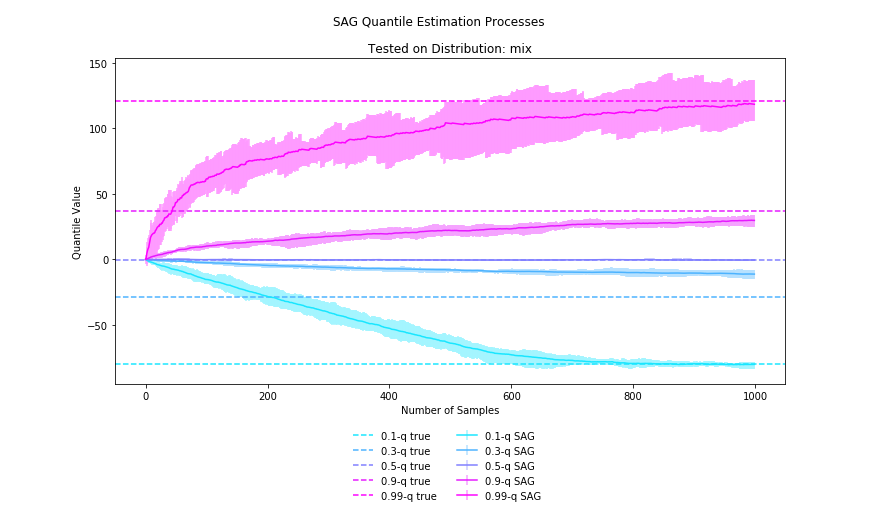
\includegraphics[width=1\columnwidth]{distro/mix_proc.png}
	\caption{SAG Process from \textit{mix} Distribution}
\end{figure}

\begin{figure}[H]
    \centering
	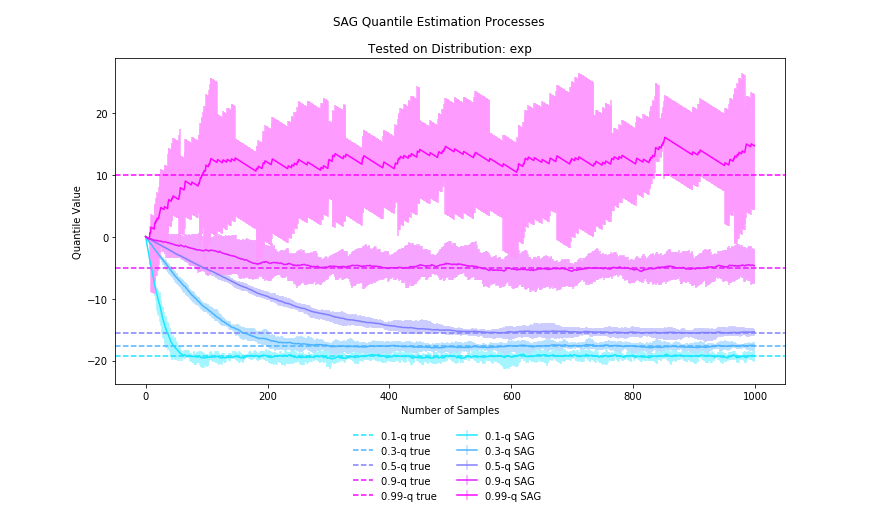
\includegraphics[width=1\columnwidth]{distro/exp_proc.png}
	\caption{SAG Process from \textit{exp} Distribution}
\end{figure}

\begin{figure}[H]
    \centering
	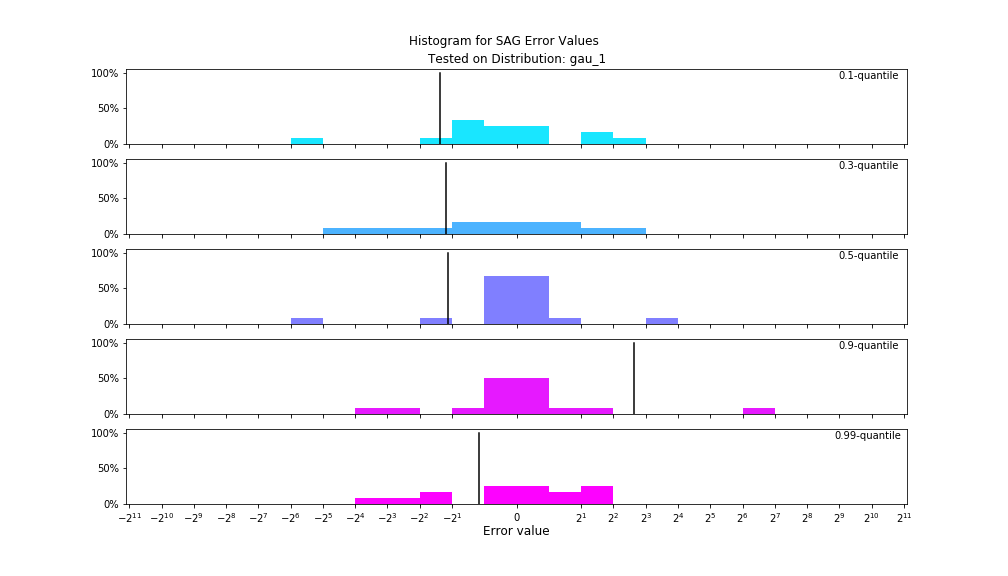
\includegraphics[width=1\columnwidth]{distro/gau_1_err.png}
	\caption{SAG Error from \textit{gau-1} Distribution}
\end{figure}

\begin{figure}[H]
    \centering
	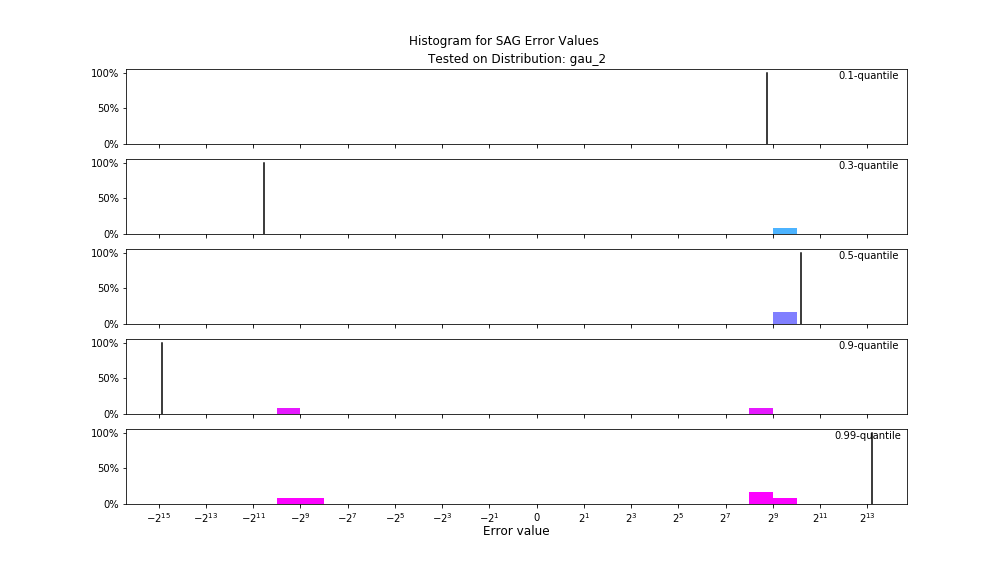
\includegraphics[width=1\columnwidth]{distro/gau_2_err.png}
	\caption{SAG Error from  \textit{gau-2} Distribution}
\end{figure}

\begin{figure}[H]
    \centering
	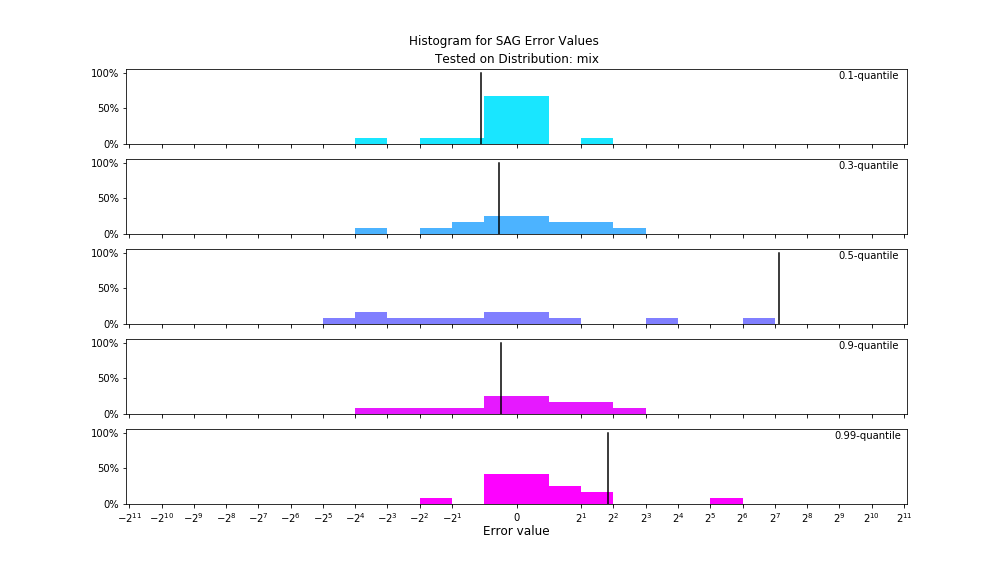
\includegraphics[width=1\columnwidth]{distro/mix_err.png}
	\caption{SAG Error from \textit{mix} Distribution}
\end{figure}

\begin{figure}[H]
    \centering
	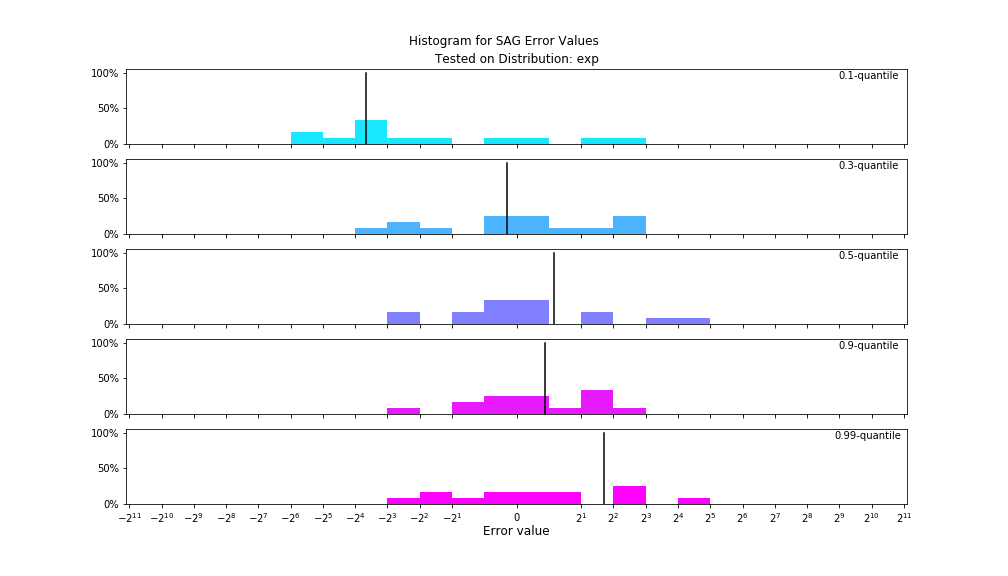
\includegraphics[width=1\columnwidth]{distro/exp_err.png}
	\caption{SAG Error from \textit{exp} Distribution}
\end{figure}

\subsection{Smooth Functions}
The pinball loss function we use for the SGD quantile estimation is convex but not smooth. 
Theoretically, however, both SGD and SAG methods need smoothness for the guarantee of convergence. Although the practical experiments have shown that there is evidence of convergence in final performance, it remains a serious problem for our SGD quantile estimation methods. In this section, we present the analysis on the non-smoothness problem, followed by the potential solutions and further discussions on them.

\subsubsection{The Pinball Loss Functions}
\graphicspath{{Figures/Stepsize_adapt/Smooth_func/}{./}} 

The pinball loss function evaluates the loss from a data point $x$ for estimation of the $\tau$-quantile.

\textbf{quote the equation of pinball loss function and it's derivative}

The fact that the pinball loss function is not differentiable at $x= 0$ has became a problem for the stochastic gradient descent which uses derivatives of object functions.

\begin{figure*}[h!]
	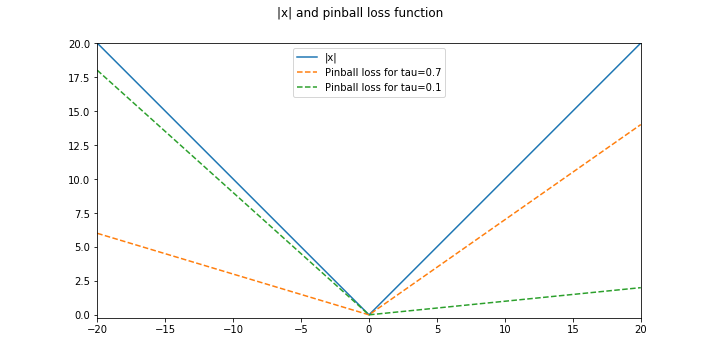
\includegraphics[width=1\columnwidth]{abs_pinball.png}
	\caption{Comparison between $|x|$ and the pinball loss function with different $\tau$ values}
\end{figure*}

The absolute function and the pinball loss function are obviously very much alike. In fact, with simple manipulation, the pinball loss function can be written in the form of absolute function as 
\begin{equation}
    l_\tau(x) = 
    \begin{cases}
        \tau \cdot |x| & {x \geq 0} \\
        (1-\tau) \cdot |x| & \text{otherwise}
    \end{cases}
\end{equation}
The pinball loss function is the combination of $|x|$ on the two parts $x<0$ and $x>0$ with different constant scale. 
If the derivative of the smooth function for $|x|$ at $x=0$ is $0$, we can also use the same approximation function respectively for the two parts of the pinball loss.
\\\\
In section \ref{subsec: smooth_sqrt} and \ref{subsec: smooth_new}, we show two approximation functions with regards to the absolute function $f = |x|$, along with the application of the approximations on the pinball loss function.

\subsubsection{Smooth function 1: a simple approxitmation}
\label{subsec: smooth_sqrt}

For $f = |x|$, a common and simple smooth approximation is $
    f = \sqrt{x^2 + \mu^2}
$.
 The convergence towards the absolute function is then proved by \citeauthor{voroninConvolutionBasedSmooth2015a}\cite{voroninConvolutionBasedSmooth2015a} that 
\begin{equation}
    ||x| - \sqrt{x^2 + \mu^2}| \leq \mu \text{  where } \mu > 0 \in \mathbb{R}
\end{equation}
\\
The smooth function application on the pinball loss function is:
\begin{equation}
    l_\tau(x) \approx 
    \begin{cases}
        \tau \cdot \sqrt{x^2 + \mu^2} & {x \geq 0} \\
        (1-\tau) \cdot \sqrt{x^2 + \mu^2} & {x < 0}
    \end{cases}
\end{equation}
and the derivative is
\begin{equation}
    l_\tau\prime(x) \approx 
    \begin{cases}
        \tau \cdot \frac{x}{\sqrt{x^2 + \mu^2}} & {x > 0} \\
        0 & {x=0} \\
        (1-\tau) \cdot \frac{x}{\sqrt{x^2 + \mu^2}} & {x<0}
    \end{cases}
\end{equation}
\subsubsection{Smooth function 2: a transcendental approximation}
\label{subsec: smooth_new}

For a better approximation accuracy, \citeauthor{bagulSMOOTHTRANSCENDENTALAPPROXIMATION2017}\cite{bagulSMOOTHTRANSCENDENTALAPPROXIMATION2017} proposes a new transcendental approximation function 
 \begin{equation}
    g(x) = x \cdot \tanh(x/\mu) \text{  where } \mu > 0 \in \mathbb{R}
 \end{equation}
which also satisfies
\begin{equation}
    ||x| - x \cdot tanh(\frac{x}{\mu})| < \mu
\end{equation}
The derivative of the approximation is
\begin{equation}
    \frac{dg(x)}{dx} = \frac{x}{\mu} \cdot sech^2 (\frac{x}{\mu}) + tanh(\frac{x}{\mu})
\end{equation}
For the pinball loss function, we now have its smooth function in the form:
\begin{equation}
    l_\tau(x) \approx 
    \begin{cases}
        \tau \cdot x \cdot \tanh(x/\mu) & {x\geq 0}\\
        (1-\tau) \cdot x \cdot \tanh(x/\mu) & {x < 0}
    \end{cases}
\end{equation}
and the derivative is
\begin{equation}
\label{eq:smooth_new_d}
    l_\tau\prime(x) \approx 
    \begin{cases}
        \tau \cdot \frac{x}{\mu} \cdot sech^2 (\frac{x}{\mu}) + tanh(\frac{x}{\mu}) & {x\geq 0}\\
        0 & {x=0}\\
        (1-\tau) \cdot \frac{x}{\mu} \cdot sech^2 (\frac{x}{\mu}) + tanh(\frac{x}{\mu}) & {x < 0}
    \end{cases}
\end{equation}
\subsubsection{Discussion and Conclusion}

In this part, we will compare the two alternative smooth functions in the following aspects: computer efficiency, approximation accuracy and
convexity. 
\begin{itemize}
    \item Computation efficiency: \\
    It is proved by \citeauthor{ramirezX2MostComputationally2014}\cite{ramirezX2MostComputationally2014} that $f = \sqrt{x^2 + \mu^2}$ is the most computationally efficient smooth approximation to $|x|$.
    
    On the other hand, we can see from equation \ref{eq:smooth_new_d}, the derivative for $g(x) = x \cdot \tanh(x/\mu)$ is more difficult to compute.
    \item Approximation accuracy: \\
    The following plots show intuitively how fast the two smooth functions approach to $|x|$ for $\mu = 0.01$ and $\mu = 0.001$.
    
    \begin{figure*}[h!]
        \includegraphics[width=1\columnwidth]{{mu_0.001}.png}
        \caption{Comparison between the two smooth functions when $\mu = 0.001$}
    \end{figure*}

    \begin{figure*}[h!]
        \includegraphics[width=1\columnwidth]{{mu_0.0001}.png}
        \caption{Comparison between the two smooth functions when $\mu = 0.0001$}
    \end{figure*}

    We can see $ x \cdot \tanh(x/\mu)$ has a better accuracy.

    \item Convexity\\
    $f = \sqrt{x^2 + \mu^2}$ is convex and  $g(x) = x · \tanh(x/\mu)$ is not.
\end{itemize}

The form of smooth function \textbf{does not really matter for SAG}. It is important to know the existence of Lipschitz continuous smooth function, and then the $L$ of such function must satisfy
\begin{equation}
    L \leq min(|\tau|, |1-\tau|)
\end{equation}
So that no matter which smooth function is used, we can simply take $min(|\tau|, |1-\tau|)$ to compute the step size $\alpha$ for SAG. However, we can still implement those smooth functions for SGD. Further researches can be done on different smooth function implementation on SGD.


\section{Doubling and Halving SGD (DH-SGD)}
\label{sec: DH_SGD}

Although SAG has a faster convergence rate than SGD, it is clear that the fluctuation problem after convergence still exists. Is it possible that a step size adaptation of SGD can minify the fluctuation after the convergence, and at the same time have an improved convergence rate? In this section, we propose a simple algorithm called Doubling and Halving Stochastic Gradient Descent (DH-SGD), which empirically improve those two problems.

\subsection{Method Description}

The idea of the DH-SGD method is trivial - increase the step size if it is too big, and decrease the step size if it is too small. We choose the change of step sizes to be exponential, specifically, increasing it to double size or decrease it to half size. The evaluation of the scale of step size can be vague.  

The psedu-code is shown here

\marginpar{THe step size scaler is different for different quantiles}
\begin{algorithm}
    \caption{DH-SGD algorithm}\label{alg:DH_SGD}
    \begin{algorithmic}[1]
        \Require{Data Stream $X$, $\tau$, $1$ unit of memory $q$, epoch check size $c$}
        \Ensure{$q$}
        % \Procedure{frugal}{$X,\tau$}            \Comment{X is the dataset}
        \State{epochCount $ec = 0$}                       \Comment{The counter for epochs}
        \State{directionCount $dc = 0$}                   \Comment{The accumulation of directions}
        \State{scaler $s = 1$}                    \Comment{The scaler for step size}
        \State {Initialize} $q$                 \Comment{Default initialization $q_0$ = 0}
        \State{}
            \For{$x_i$ in $X$}                  \Comment{Parameter update for each input data point}
                \State{}
                \State{$ec = ec+ 1$}   
                \If{$ec$ \textit{mod} $c = 0$}            \Comment{Change scaler for every $c$ epochs}
                    \If{$|dc| > 0.25c$ }               
                        \State{$s = 2s$}               \Comment{Double $s$ if the update is mostly in one direction}         
                    \Else {\textbf{if} $|dc| < 0.02c$ \textbf{then}}  
                        \State{$s = 0.5s$}             \Comment{Halve $s$ if the update direction barely changes}
                    \EndIf
                
                \EndIf
                \State{}
                \State{\textbf{set} $\alpha_i = 1$}             \Comment{$\alpha_i$ can use other settings}
                \State{$\alpha_i = \alpha_i \cdot s$}        \Comment{Scale original step size with $s$}
                \If{$x_i > q$}                  
                    \State{$q = q + \alpha_i \tau$}
                    \State{$dc = dc + 1$}                   \Comment{Direction count $+1$ if updated upwards}
                \Else {\textbf{if} $x_i < q$ \textbf{then}}                     
                    \State{$q = q - \alpha_i (1-\tau)$}
                    \State{$dc = dc -1$}                    \Comment{Direction count $-1$ if updated downwards}

                \EndIf
            \EndFor
        \State{}
        \State \textbf{return} $q$
        % \EndProcedure
    \end{algorithmic}
\end{algorithm}

\subsection{Experiments}
\graphicspath{{Figures/Stepsize_adapt/Adaptive_stepsize/}{./}} 

Interesting Observations:

\begin{enumerate}
    \item The change of step size "does not always work". Works: other, \textit{gau-2} obvious but still not quite working, not work: $0.99$-q \textit{exp}
    \item Fluctuation does change, but is sometimes worse (\textit{gau-1} $0.1$-q $0.3$-q Error outlier) No guarantee of convergence? a really big problem
\end{enumerate}
\subsubsection{DH-SGD on Different Distributions}
\label{subsubsec: DH_SGD_exp_distro}
\begin{figure}[H]
    \centering
	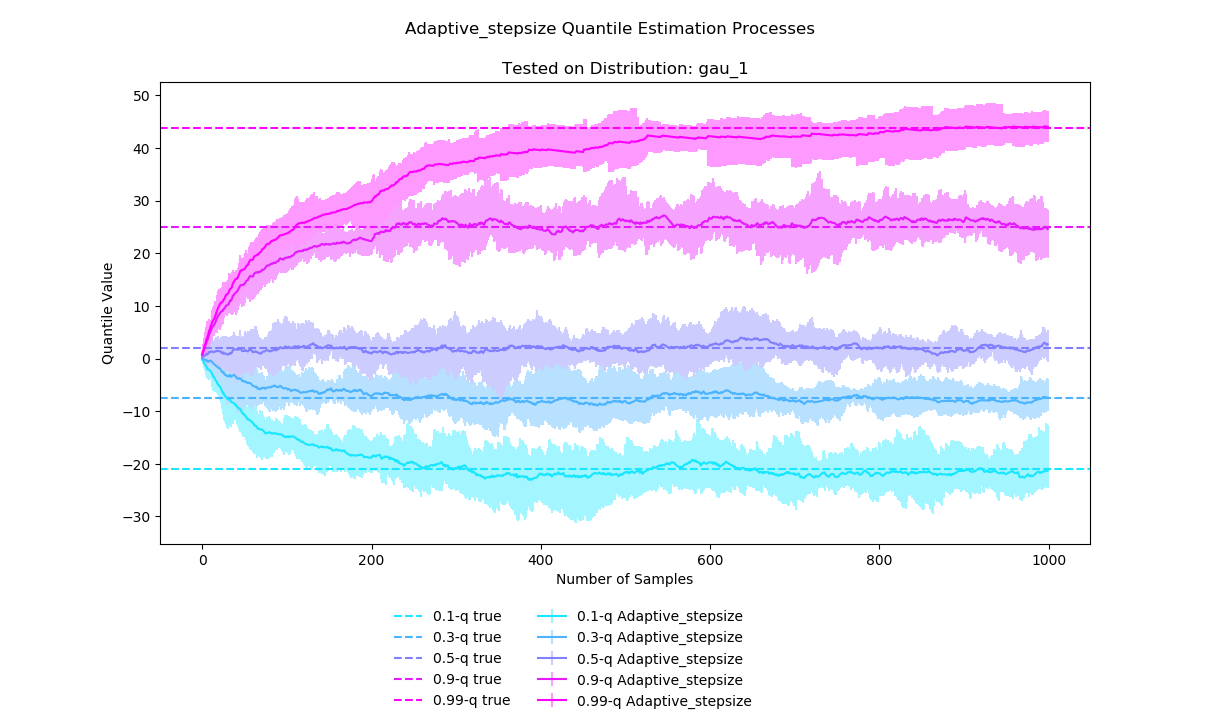
\includegraphics[width=1\columnwidth]{distro/gau_1_proc.png}
	\caption{DH-SGD Process from \textit{gau-1} Distribution}
\end{figure}

\begin{figure}[H]
    \centering
	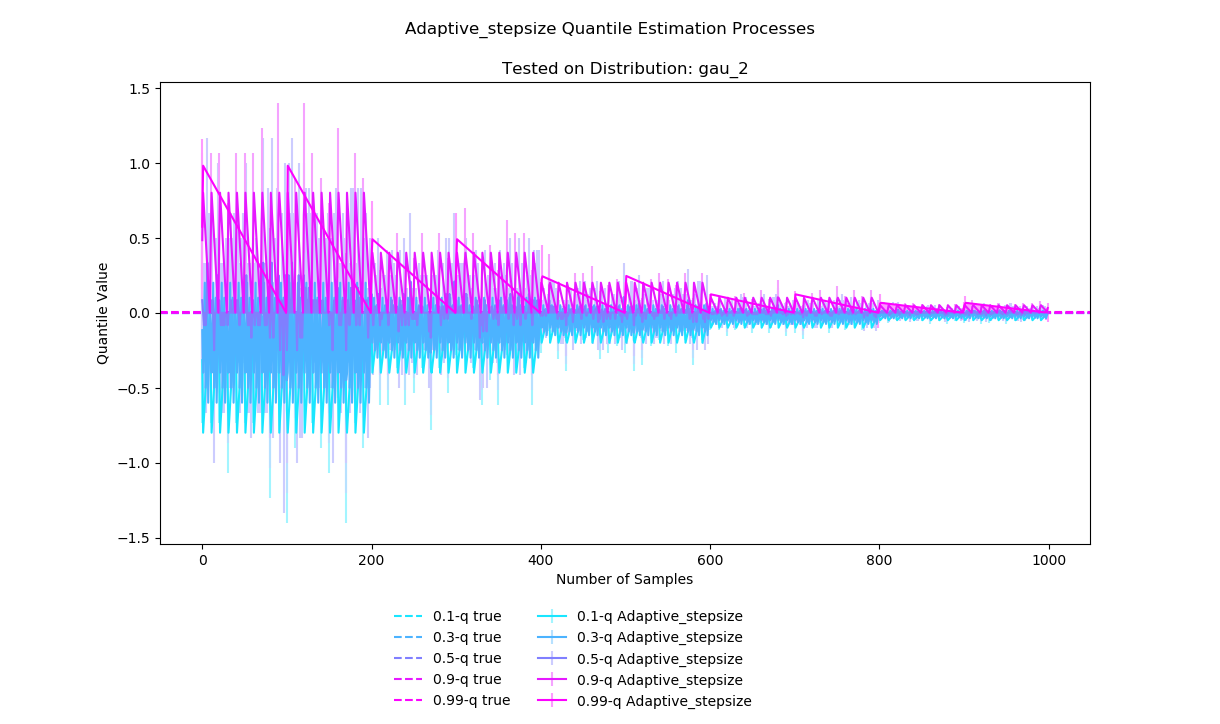
\includegraphics[width=1\columnwidth]{distro/gau_2_proc.png}
	\caption{DH-SGD Process from  \textit{gau-2} Distribution}
\end{figure}

\begin{figure}[H]
    \centering
	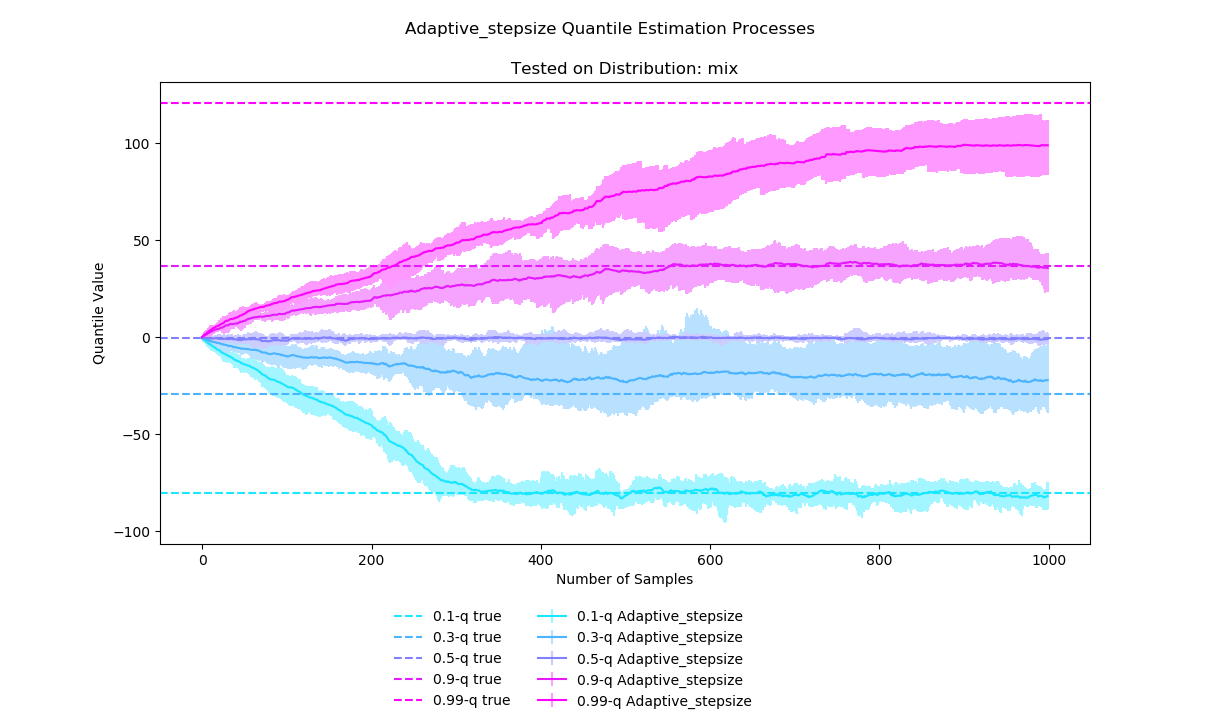
\includegraphics[width=1\columnwidth]{distro/mix_proc.png}
	\caption{DH-SGD Process from \textit{mix} Distribution}
\end{figure}

\begin{figure}[H]
    \centering
	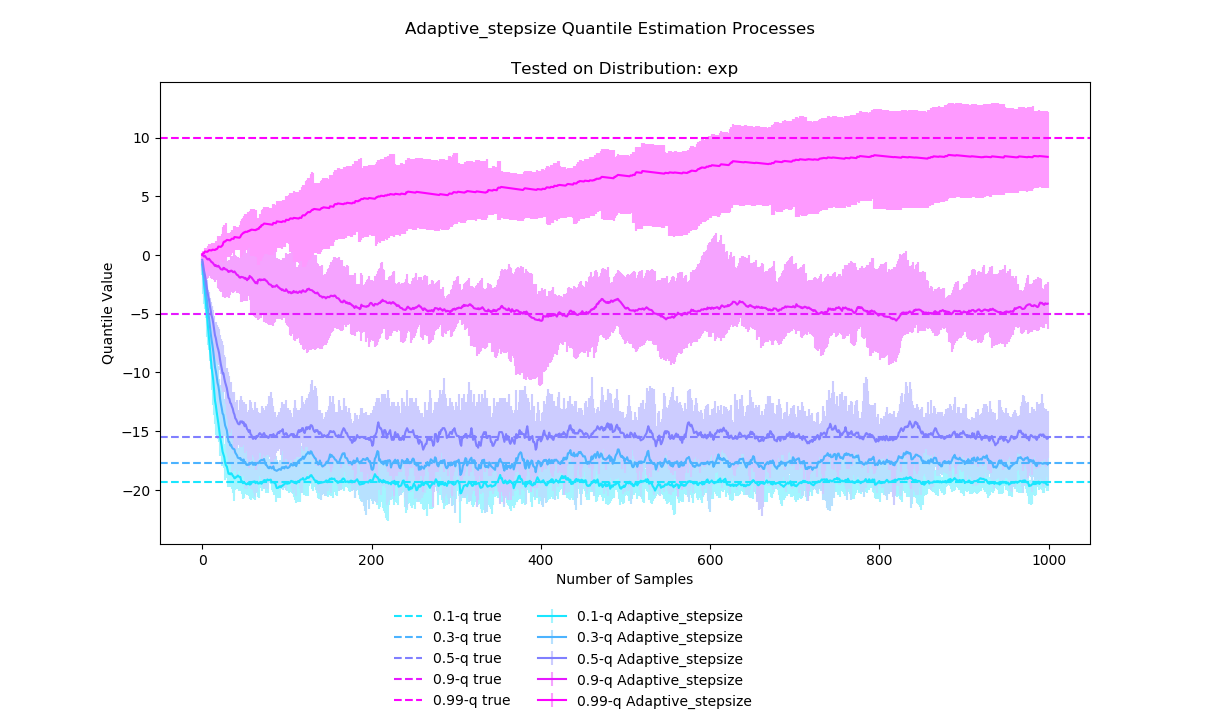
\includegraphics[width=1\columnwidth]{distro/exp_proc.png}
	\caption{DH-SGD Process from \textit{exp} Distribution}
\end{figure}

\begin{figure}[H]
    \centering
	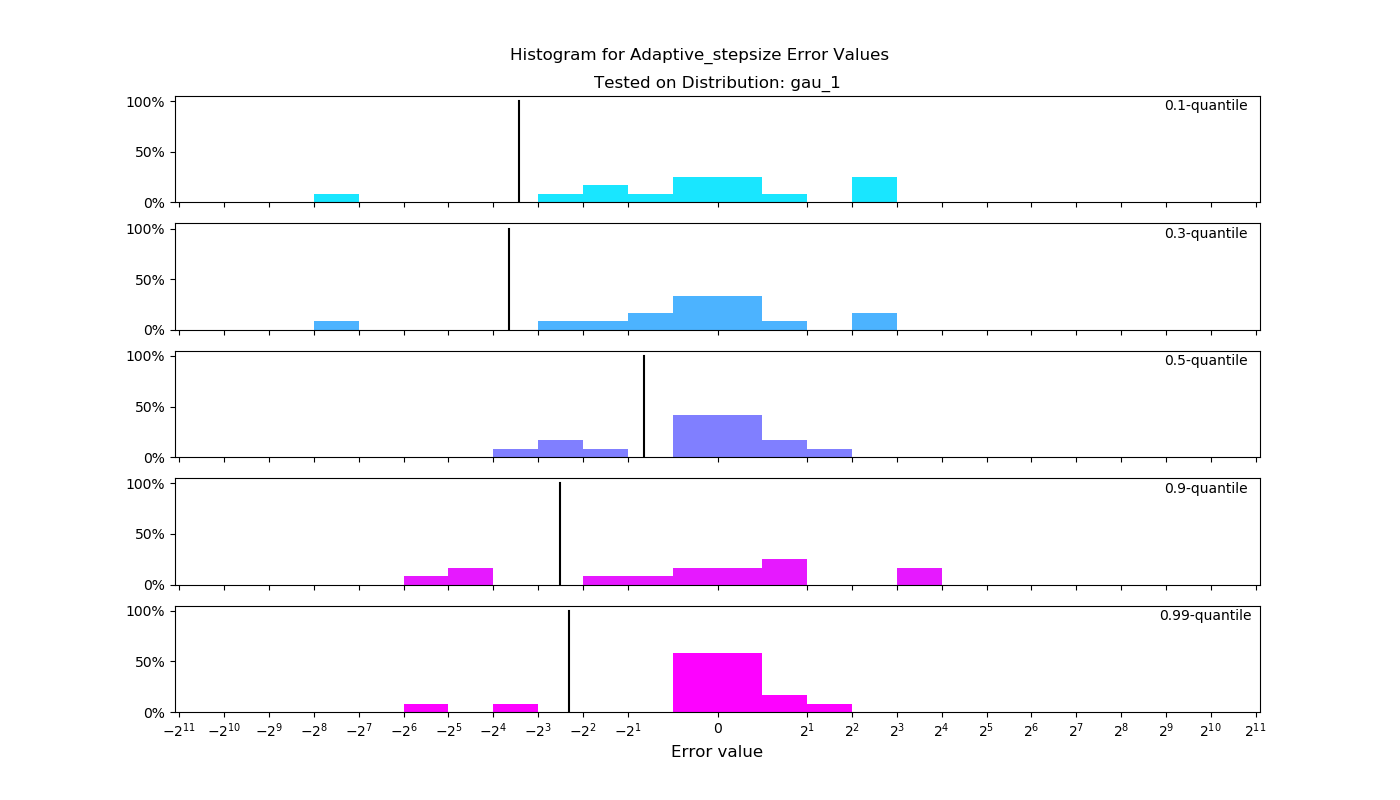
\includegraphics[width=1\columnwidth]{distro/gau_1_err.png}
	\caption{DH-SGD Error from \textit{gau-1} Distribution}
\end{figure}

\begin{figure}[H]
    \centering
	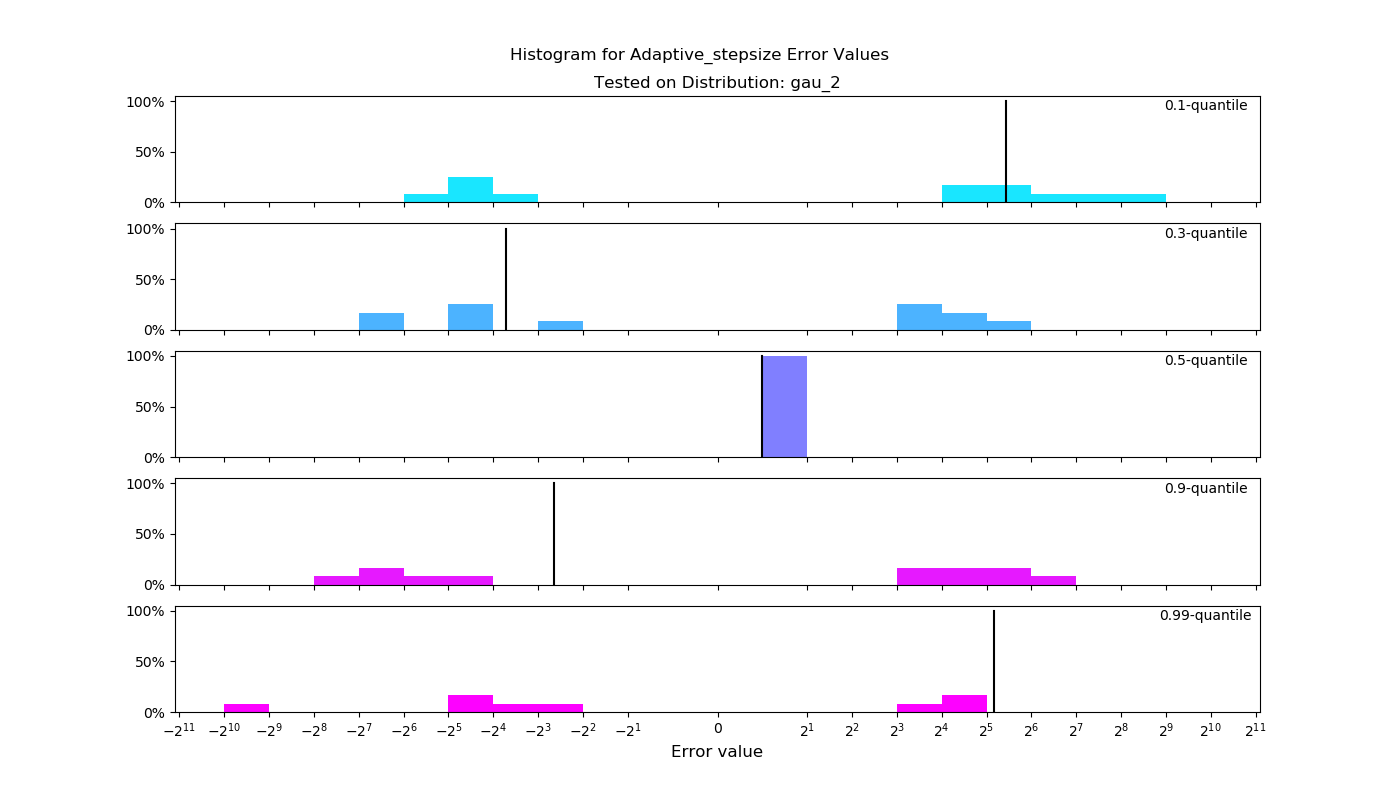
\includegraphics[width=1\columnwidth]{distro/gau_2_err.png}
	\caption{DH-SGD Error from  \textit{gau-2} Distribution}
\end{figure}

\begin{figure}[H]
    \centering
	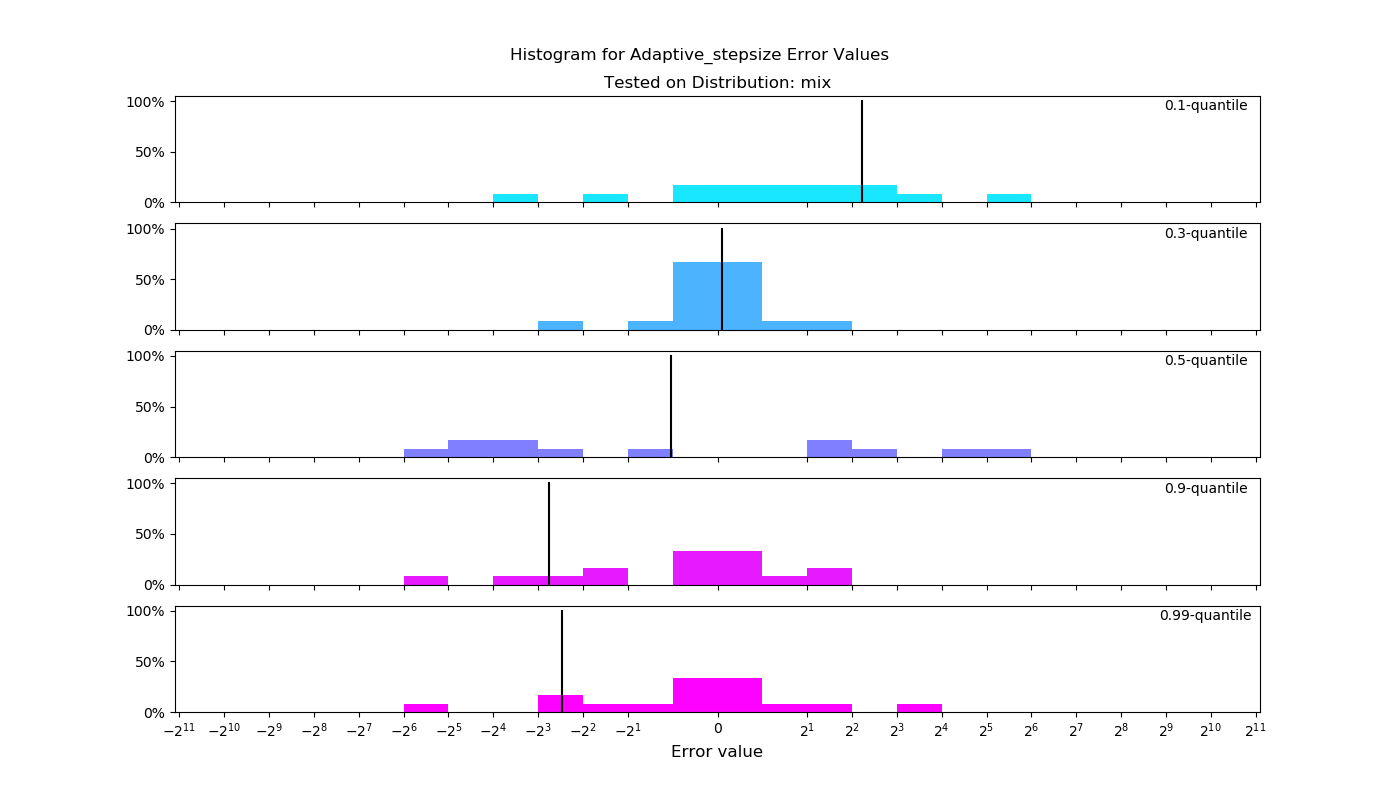
\includegraphics[width=1\columnwidth]{distro/mix_err.png}
	\caption{DH-SGD Error from \textit{mix} Distribution}
\end{figure}

\begin{figure}[H]
    \centering
	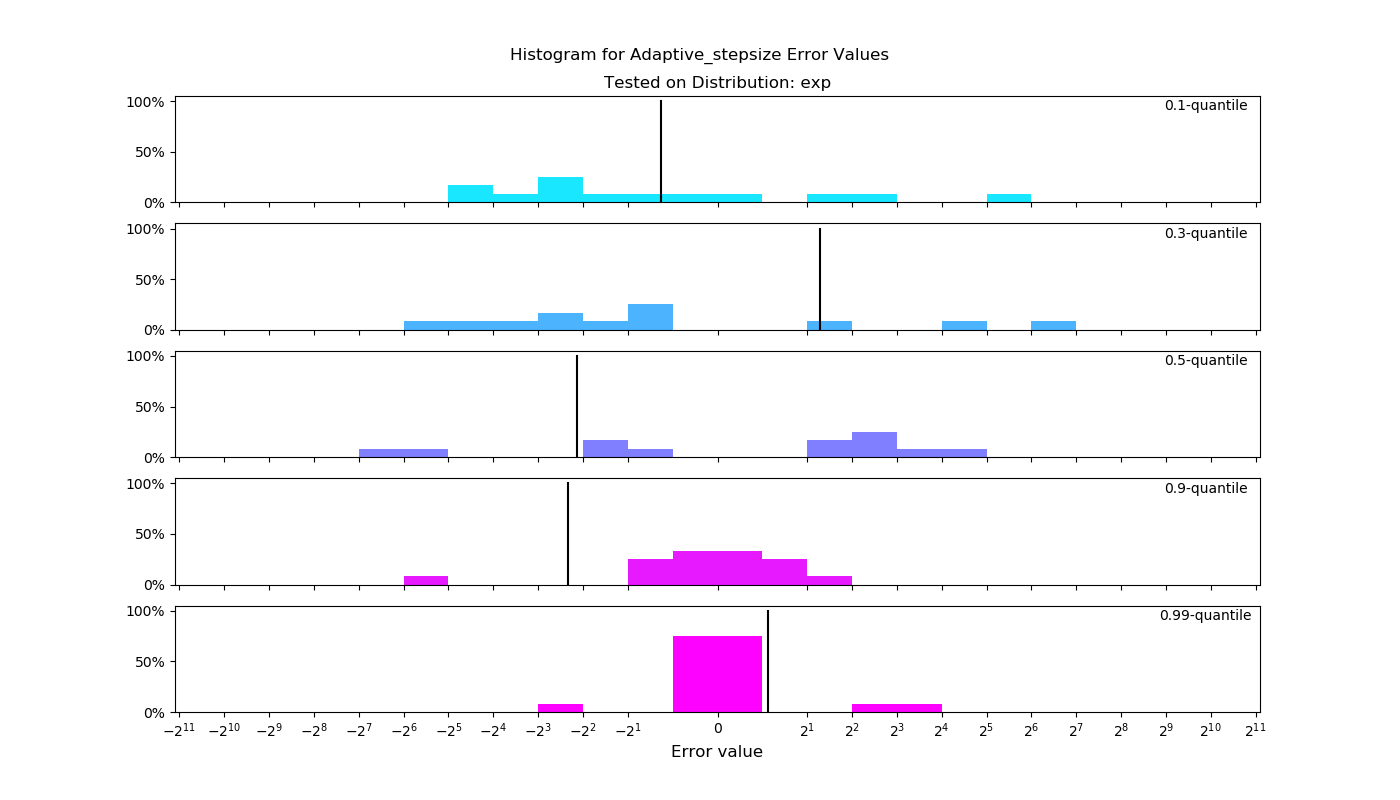
\includegraphics[width=1\columnwidth]{distro/exp_err.png}
	\caption{DH-SGD Error from \textit{exp} Distribution}
\end{figure}

\subsubsection{DH-SGD on Different Data Size}
\label{subsubsec: DH_SGD_exp_data_size}

\begin{figure}[H]
    \centering
	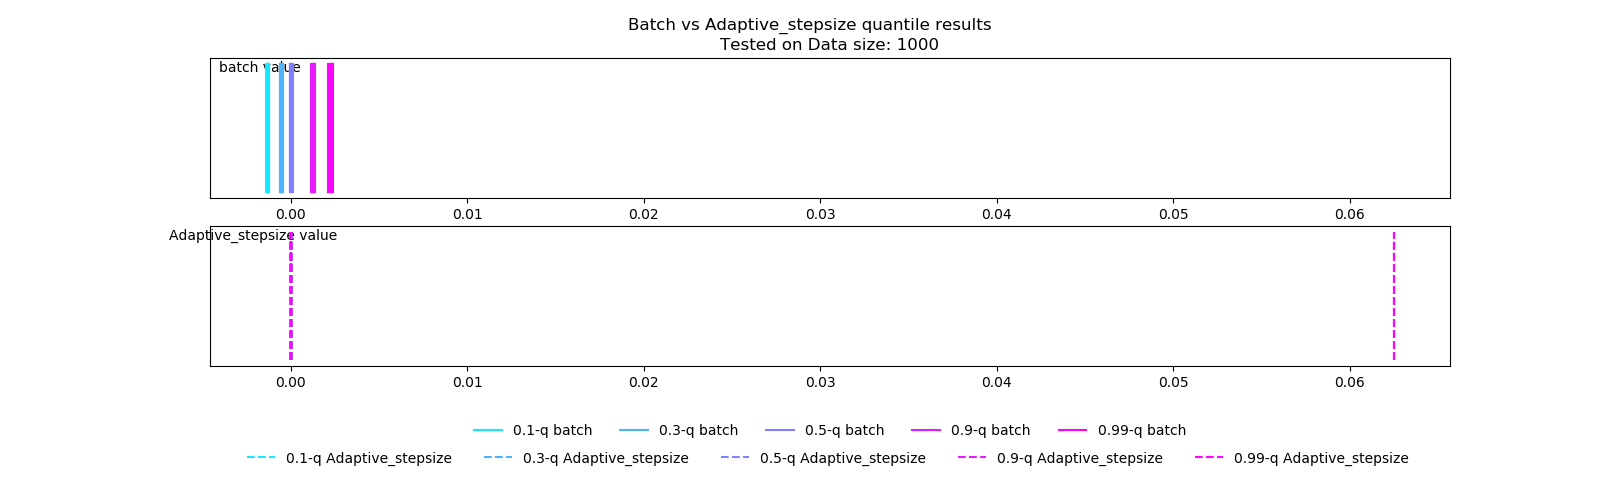
\includegraphics[width=1\columnwidth]{data_size/1000_res.png}
	\caption{DH-SGD Results from 1000 samples from \textit{gau-2} Distribution}
\end{figure}

\begin{figure}[H]
    \centering
	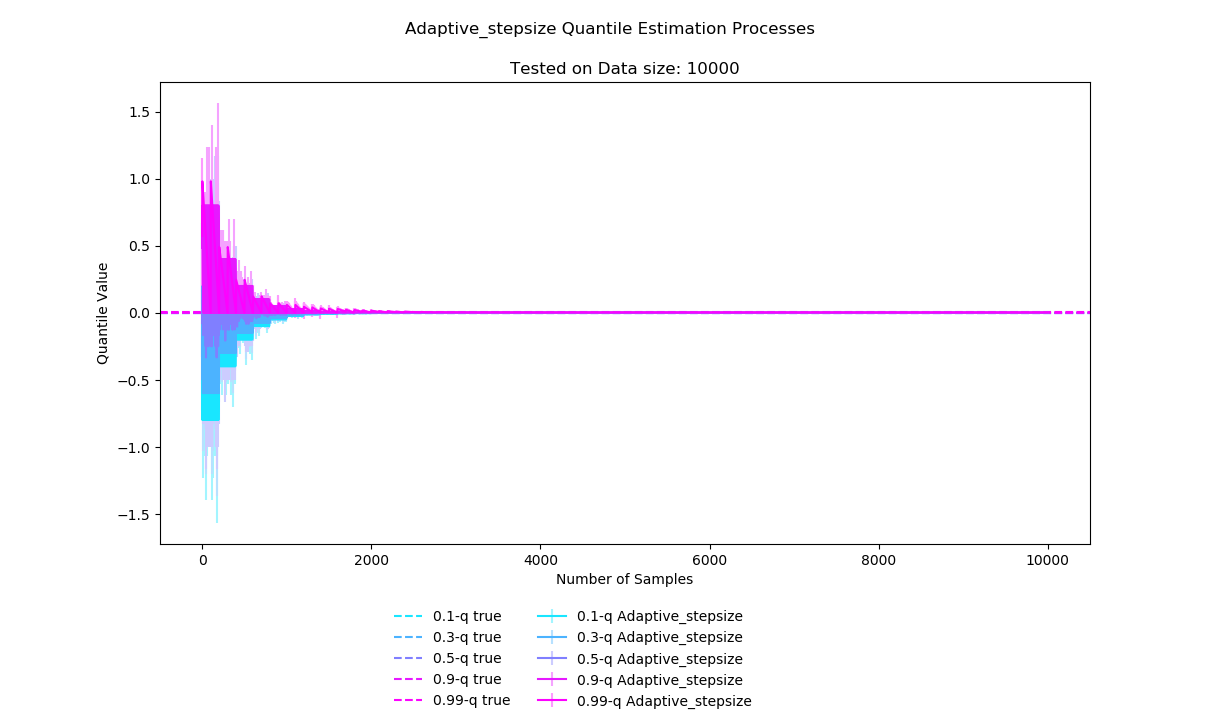
\includegraphics[width=1\columnwidth]{data_size/10000_proc.png}
	\caption{DH-SGD Process from 10000 samples from\textit{gau-2} Distribution}
\end{figure}

\begin{figure}[H]
    \centering
	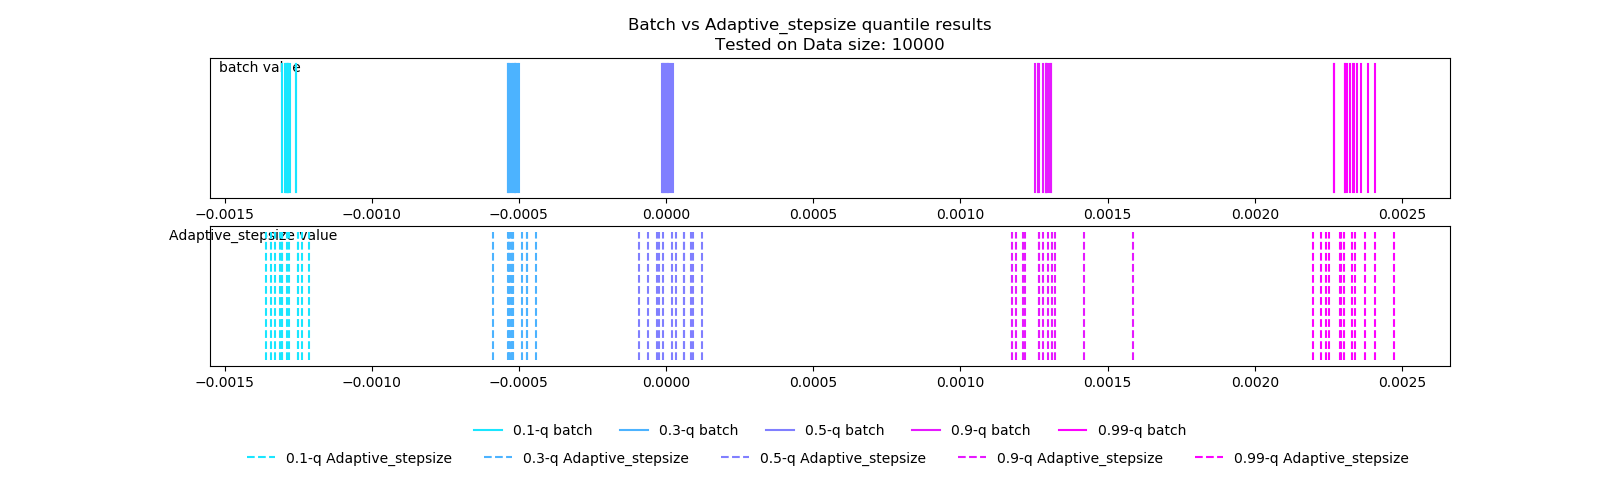
\includegraphics[width=1\columnwidth]{data_size/10000_res.png}
	\caption{DH-SGD Results from 10000 samples from \textit{gau-2} Distribution}
\end{figure}

\begin{figure}[H]
    \centering
	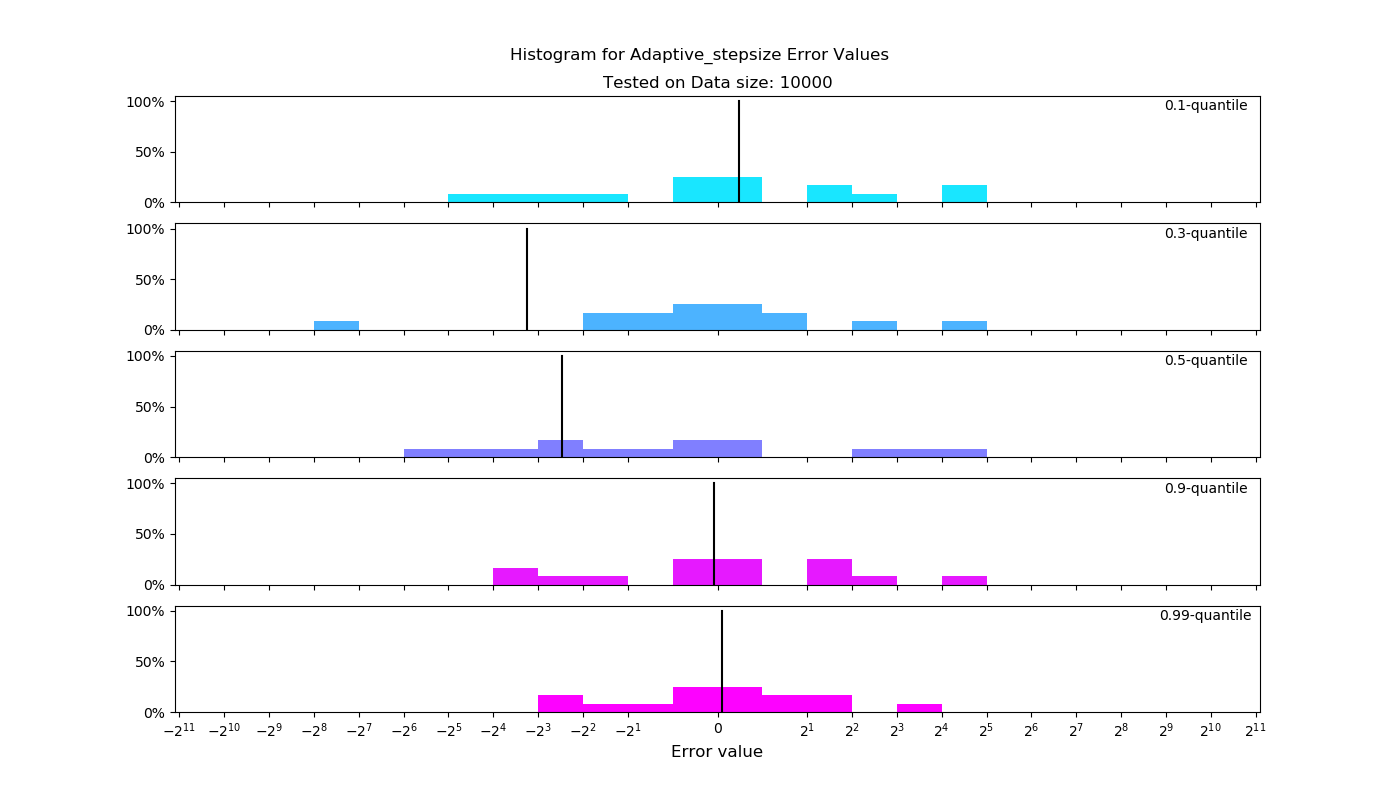
\includegraphics[width=1\columnwidth]{data_size/10000_err.png}
	\caption{DH-SGD Error from 10000 samples from \textit{gau-2} Distribution}
\end{figure}

\subsection{Discussion}

Choice on \textbf{step size check}:
    If step size check to be small: easier to have gau-2 converge within 1000 epochs, but not enough data for epoch checking
    If step size check large: the other way around
    Since we assume the data stream is big, maybe try with more than 200 epochs

    (try a different way) Can actually get easily solved by sorting the first F (F = 100 for example) quantiles and set the initialization and step size according to that

The judgement of\textbf{ "too small/big"} step size: 
    binomial distro for different quantiles The possibility that there are exactly $x$ epochs  going up in the total of $n$ epochs for $\tau$ when the quantile has converged.
    The distribution is different for different $\tau$ and different $n$, but $n$ does not matter that much as $\tau$ in this situation. It means the distance between of \textbf{dfa} should be different for different $\tau$.


\section{Discussion and conclusion}

Compare SAG, Doubling-and-Halving SGD and SGD

Conclusion: both are good methods lol

1. Convergence rate:

2. Fluctuation after convergence

5. Further improvement: SAG + DH SGD?

% \chapter{Smooth Functions}
\label{ch: smooth_func}

\textbf{This is a section not a chapter}


\section{Smooth Functions}
The pinball loss function we use for the SGD quantile estimation is convex but not smooth. 
Theoretically, however, both SGD and SAG methods need smoothness for the guarantee of convergence. Although the practical experiments have shown that there is evidence of convergence in final performance, it remains a serious problem for our SGD quantile estimation methods. In this section, we present the analysis on the non-smoothness problem, followed by the potential solutions and further discussions on them.

\subsection{The Pinball Loss Functions}
The pinball loss function evaluates the loss from a data point $x$ for estimation of the $tau$-quantile.
% \algnewcommand{\LineComment}[1]{\State \(\triangleright\) #1}
% New definitions
\algnewcommand\algorithmicswitch{\textbf{switch}}
\algnewcommand\algorithmiccase{\textbf{case}}
\algnewcommand\algorithmicassert{\text{assert}}
\algnewcommand\Assert[1]{\State \algorithmicassert(#1)}%
% New "environments"
\algdef{SE}[SWITCH]{Switch}{EndSwitch}[1]{\algorithmicswitch\ #1\ \algorithmicdo}{\algorithmicend\ \algorithmicswitch}%
\algdef{SE}[CASE]{Case}{EndCase}[1]{\algorithmiccase\ #1}{\algorithmicend\ \algorithmiccase}%
\algtext*{EndSwitch}%
\algtext*{EndCase}%

% \graphicspath{{Figures/Multi/P2/}{./}} 

\chapter{Simultaneous Multiple Quantile Estimation}
\label{ch: multi_quant}

\graphicspath{{Figures/Multi/}{./}} 

The previously introduced methods estimate only a single quantile. For applications which need multiple quantiles, these methods are not sufficient.\marginpar{This opening phrase is still not very good.}
In this chapter we introduce the problem of simultaneous multi-quantile estimation and two related methods. The structure is organised as follow:

Section~\ref{sec: multi_intro} introduces the multi-quantile estimation for streaming data, followed by a discussion on the basic ideas to approach this problem. The next two sections will show how it is solved by methods focusing on different aspects.

Section~\ref{sec: multi_shiftQ} shows the \textit{shiftQ} algorithm for simultaneous quantile estimation by implementing an idea similar to SGD.

Section~\ref{sec: multi_{p2}} shows the \textit{$P^2$} algorithm that solves the problem in a different way.

% Section~\ref{sec: multi_discussion} compares and contrasts the two methods, the discussion about the problem and our conclusion.

\section{The problem and opportunity of multi-quantile estimation}
\label{sec: multi_intro}

In real life implementations, quantile estimation usually does not focus on a single quantile value. For example, a common request is to show the median (the $0.5$-quantile) of the distribution, and at the same time show the outlier boundaries at ends of the distribution, like the $0.1$- and $0.9$- quantiles. It is also likely that multiple quantile estimates are required for a data distribution analysis.

\begin{figure}[h]
    \centering
	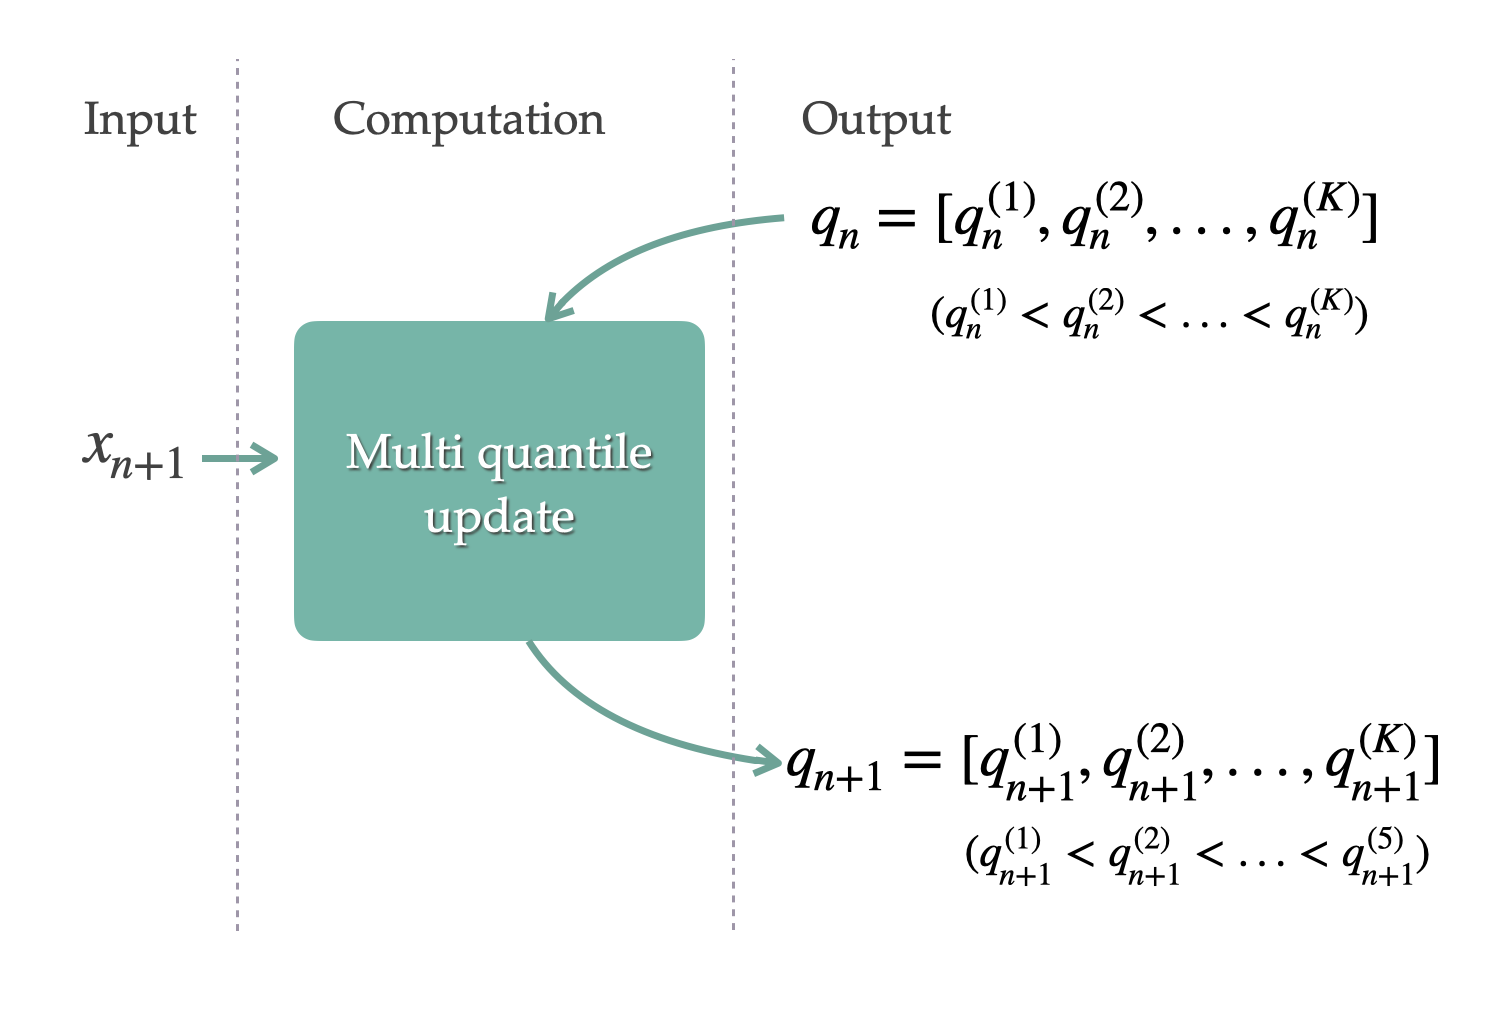
\includegraphics[width=0.7\columnwidth]{Multi_img.png}
	\caption{The update of multi-quantile estimation methods in general}
\end{figure}

A trivial solution for multi-quantile estimation is to run multiple single quantile estimation processes in parallel, such that each quantile is estimated by one process. The multi-process solution however, leads to two main problems:
\begin{enumerate}
    \item The application software/hardware might not have sufficient parallel processing capacity for the algorithm.
    \item Estimating the quantiles independently means the monotone property of quantiles is not taken into account. That is, $\tau_1$-$q > \tau_2$-$q$ if and only if $\tau_1 > \tau_2.$
\end{enumerate}

The following two multi-quantile estimation methods can simultaneously estimate multiple quantile values in one process while utilising the monotonic property. Both algorithms, \textit{shiftQ}\cite{hammerJointTrackingMultiple2019b} and \textit{extended $P^2$}\cite{raatikainenSequentialProcedureSimultaneous1993} utilize the monotone property by ensuring a positive distance between one quantile and its previous quantile, i.e.,
$q_{i} - q_{i-1} > 0$. The shiftQ algorithm is described in section \ref{sec: multi_shiftQ}, and the next section \ref{sec: multi_{p2}} for the extended $P^2$ algorithm.



% ----------------------------------- shiftQ ---------------------------------------

\section{The shiftQ method}
\label{sec: multi_shiftQ}

In general, shiftQ updates its quantile estimates each time a new observation is made. Each update of the algorithm consists of the update of a central quantile followed by updating each other quantile outwards from the center. The central point is updated with the \emph{deterministic update-based multiplicative incremental quantile estimator} (DUMIQE) and the latter are updated using the concept of \emph{shifted distributions}. In this section, we first briefly introduce the DUMIQE algorithm, followed by an explanation of shifted distributions and section \ref{subsec: multi_shiftQ_description} details how the shitQ algorithm uses these concepts to estimate multiple quantile simultaneously.
\\\\
The DUMIQE algorithm updates the quantile estimate upon the arrival of each new observation. It is a development on the work of \citeauthor{tierneySpaceEfficientRecursiveProcedure1983}\cite{tierneySpaceEfficientRecursiveProcedure1983}, which applies a stochastic approximation on quantile estimation. The similarity between DUMIQE and SGD can be seen in the following algorithm pseudo-code:

\begin{algorithm}
    \caption{DUMIQE algorithm}\label{alg:DUMIQE}
    \begin{algorithmic}[1]
        \Require{Data Stream $X$, stepsize $\alpha$}, $\tau$, initial quantile estimate $q_0$ ($q_0 > 0$)
        \Ensure{$q$}
        % \Procedure{frugal}{$X,\tau$}            \Comment{X is the dataset}
        % \State {Initialize} $q$                 \Comment{Requires \textbf{positive initialization} $q$ > 0}
        \State{$q = q_0$}                         \Comment{\textbf{Positive} initialization }
            \For{$x_k$ in $X$}                  \Comment{Parameter update for each input data point}
                % \State \textbf{set} $\alpha_k$  \Comment{Set stepsize}
                \If{$x_k > q$}                  
                    \State{$q = q + \alpha \tau \cdot q$}
                \Else                           
                    \State{$q = q - \alpha (1-\tau)\cdot q$}
                \EndIf
            \EndFor
        \State \textbf{return} $q$              \Comment{$q$ is the DUMIQE estimation result}
    \end{algorithmic}
\end{algorithm}

The update of other quantiles are based on the the relationship with the central quantile. For example, if the central quantile is the median, the $0.25$-quantile is then estimated as the median of distribution below the estimate of median. To apply this idea, DUMIQE uses a shifted distribution $Y$ of the input $X$ such that $X = Y + \delta$, where $\delta$ is the shift constant. In the following method description, we use $Q_X(q)$ and  $Q_Y(q)$ to denote the estimate of $q$ on distribution $X$ and $Y$. In order to distinguish the quantile estimate on different distributions, the DUMIQE algorithm for the $\tau_k$-quantile on distribution $X$ at the observation of the $n$th sample $x_n$ is written as \marginpar{cases to be added to equation}
\begin{align}
        &Q_{X, n+1}(q_k) \leftarrow Q_{X, n}(q_k) + \alpha \tau_k \cdot Q_{X, n}(q_k)  & \text{if } Q_{X, n}(q_k) < x_n \\
        &Q_{X, n+1}(q_k) \leftarrow Q_{X, n}(q_k) - \alpha (1-\tau_k) \cdot Q_{X, n}(q_k)  & \text{if } Q_{X, n}(q_k) \geq x_n \nonumber
\end{align}

\subsection{Method Description}
\label{subsec: multi_shiftQ_description}

\textbf{Motivation}: The difference between the two quantiles for the $x_{n}$ observation is:
$$
diff = |Q_{X,n}(q_{k+1}) - Q_{X,n}(q_k)|
$$
Note that $diff > 0$ for all $x_i, i \in \{1,...,N\}$, so different quantiles never cross each other. This property is guaranteed by the update function DUMIQE() and its restriction that the input quantile estimate must be positive.
\\\\
At the arrival of observation $x_n$, the central quantile estimate $q_c$ is first updated. Denote $K$ as the number of quantiles for estimation. Then the quantile estimates smaller than $q_c$ are updated based on the nearest quantile larger than them, yielding the sequence $\{q_{c-1}, ..., q_1\}$, and conversely the bigger quantile estimates are updated in the order of {$q_{c+1}, ..., q_{K}$}.
\\\\
\textbf{Updating one quantile:} The difference between a quantile $q_{k+1}$ and its neighbour $q_k$ is calculated based on the idea of a "shifted distribution".
Let $X$ denote the original distribution of the data stream, and let the distribution $Y$ denote a shifted version of $X$ such that $Y = X + \delta$ for some constant $\delta$. In this way, the quantile estimate $q_{k+1}$ can be updated by implementation of shifting. The basic steps are:
        \begin{enumerate}
            \item Calculate the shift constant $\delta = Q_{X,n}(q_k)$
            \item Get shifted observation $y_{n,k+1} =  \delta - x_n$ \label{step: shift_observation}
            \item Use the shifted observation to calculate the shifted quantile estimate $Q_{Y, n+1}(q_{k+1})$ with DUMIQE
            \item Shift back to $X$: $Q_{X,n+1}(q_{k+1}) =  \delta  - Q_{Y, n+1}(q_{k+1})$
        \end{enumerate}
When updating a quantile $q_{k-1}$ based on $q_k$, step \ref{step: shift_observation} uses the inverse: $y_{n,k-1} = x_n - \delta$
\\\\
\noindent\textbf{shiftQ update:}
The steps of the shiftQ algorithm are:
\begin{enumerate}
    \item \textbf{Update the central quantile:} Calculate $q_c = Q_{X,n+1}(q_c)$ by DUMIQE 
    \item \textbf{Update the smaller quantiles:} Starting from central quantile $q_c$, the estimates for $q_{c-1}, ..., q_{1}$ are calculated each based on the last.
    \item  \textbf{Update the bigger quantiles:} Similar to step 2, the larger quantiles are estimated for $q_{c+1}, ..., q_{K}$ in sequence.
\end{enumerate}

Pseudocode for the shiftQ algorithm is included as algorithm \ref{alg:multi_shiftQ}.
% \subsection{The shiftQ Algorithm}
\begin{algorithm}
    \caption{The shiftQ Algorithm}\label{alg:multi_shiftQ}
        \begin{algorithmic}[1]
            \Require
            \State{Dataset $X$ (with positive data points only)}
            \State{Target quantile values $[\tau_1, \tau_2, ..., \tau_K]$}
            \State{Central position $c$, Number of quantiles $K$}
            \State{Stepsize $\alpha_X$, Stepsize $\alpha_Y$}
            \State{Quantile Estimate Initialization on $X$: {$0 < Q_{X,0}(q_1) < ... < Q_{X,0}(q_K)$}}
            \State{Quantile Estimate Initialization on $Y$: {$0 < Q_{Y,0}(q_1) < ... < Q_{Y,0}(q_K)$}}
            \Ensure{Target quantile estimates $[\tau_1\text{-}q, \tau_2\text{-}q, ..., \tau_K\text{-}q]$}

            \State
            \State{Choose some $c \in {1,..K}$, usually the middle point}
            \State{$q_c \gets Q_{X,0}(q_c)$}
            \For{$x_n \in X$}
                \LineComment{Update central quantile}
                \State{$q_c \leftarrow DUMIQE(q_c, x_n, \tau_c, \alpha_X)$}
                \State{}

                \For{$k \in \{c-1, ..., 1\}$}
                \LineComment{Update smaller quantiles}
                    \State{$\delta \leftarrow Q_{X,n+1}(q_{k+1})$}
                    \State{$y_{n,k+1} \leftarrow Q_{X,n}(q_{k+1}) - x_n$}
                    \State{$Q_{Y, n+1}(q_{k}) \leftarrow DUMIQE(Q_{Y, n}(q_{k}), y_{n,k+1}, q_k, \alpha_Y)$}
                    \State{$Q_{X,n+1}(q_{k}) \leftarrow \delta - Q_{Y, n+1}(q_{k+1})$}
                \EndFor
                \State{}

                \For{$k \in \{c+1, ..., K\}$}
                \LineComment{Update bigger quantiles}
                    \State{$\delta \leftarrow Q_{X,n+1}(q_{k-1})$}
                    \State{$y_{n,k-1} \leftarrow  x_n - Q_{X,n}(q_{k-1})$}
                    \State{$Q_{Y, n+1}(q_{k}) \leftarrow DUMIQE(Q_{Y, n}(q_{k}), y_{n,k-1}, q_k, \alpha_Y)$}
                    \State{$Q_{X,n+1}(q_{k}) \leftarrow \delta + Q_{Y, n+1}(q_{k-1})$}
                \EndFor
            \EndFor

            \State
            \LineComment{Return final estimaton}
            \State{$[\tau_1\text{-}q, \tau_2\text{-}q, ..., \tau_K\text{-}q] \leftarrow [Q_{X,N}(q_1), ..., Q_{X,N}(q_K) ]$}
        \end{algorithmic}
\end{algorithm}
\subsection{Experiment Results}

There are two experiments run on shiftQ algorithm. Refer to \textcolor{blue}{insert chapter reference here} for the details of the experiment settings. The first one aims to compare the quantile crossing behaviour of shiftQ and SGD, and the second one tests shiftQ's performance on quantile estimation.

In the first experiment, the experiment dataset is 5000 samples generated from a uniform distribution over the range $(0,100)$. All data points are required to be positive as the prerequisite of the shiftQ algorithm. This experiment compares two algorithms, shiftQ and SGD, and examines the quantile crossing behaviour of each algorithm.

\marginpar{Fig \ref{fig: shiftQ_SGD} graphic needs axis labels}
\begin{figure}[h!]
	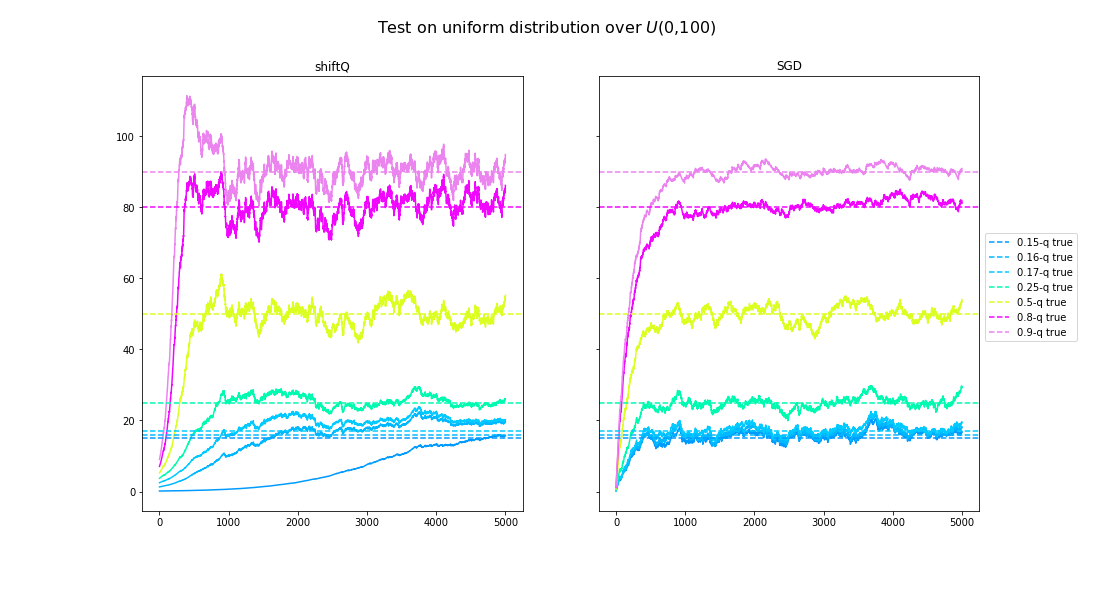
\includegraphics[width=1\columnwidth]{shiftQ/shiftQ_vs_SGD.png}
    \caption{Two process plots comparing the estimation of quantiles 0.15-q, 0.16-q, 0.17-q, 0.25-q, 0.8-q and 0.9-q with shiftQ and SGD over a uniform distribution.}
    \label{fig: shiftQ_SGD}
\end{figure}

\marginpar{``epoch'' terminology under review}
Figure \ref{fig: shiftQ_SGD} shows the estimates by shiftQ and SGD over 5000 epochs in the first experiment. In this experiment, $0$ crossings occurred in the shiftQ implementation, while SGD caused 33 crossings. Over 100 repetitions of this experiment, the average number of crossings by SGD is 72.48, with a standard deviation of 66.23. The crossings in SGD have two interesting properties:
    \begin{enumerate}
        \item The crossings are likely to occur when two quantile values are close to each other. For example, in this example, only two pairs of quantiles ($0.15$, $0.16$) and ($0.16$, $0.17$) are detected to have crossings. The difference between the true quantile values of these pairs is 1, while the other adjacent quantile pairs are at least 8 away from each other. Given the stepsize was set to $\alpha = 0.45$ for SGD, the short distance between two adjacent quantile values are likely to be the main cause of crossings.
        \item The crossings happen are likely to happen in a slot of concentrated continuous epochs. For example, among the 33 crossings, 11 of them are between $0.16$-q and $0.17$-q from epoch 2400 to 2410. The other 22 crossings are between $0.15$-q and $0.16$-q continuously from epoch 3489 to 3510. This suggests that once a crossing takes place, its impact is likely to continue for the following epochs until the crossing is fixed.
    \end{enumerate}

The second experiment aims to investigate the effectiveness of shiftQ algorithm. Figures \ref{fig: shiftQ_proc}, \ref{fig: shiftQ_res} and \ref{fig: shiftQ_err} show process plots for the shiftQ algorithm run on the absolute value of 1000 samples from \textit{gau-1}.

\begin{figure}[h!]
	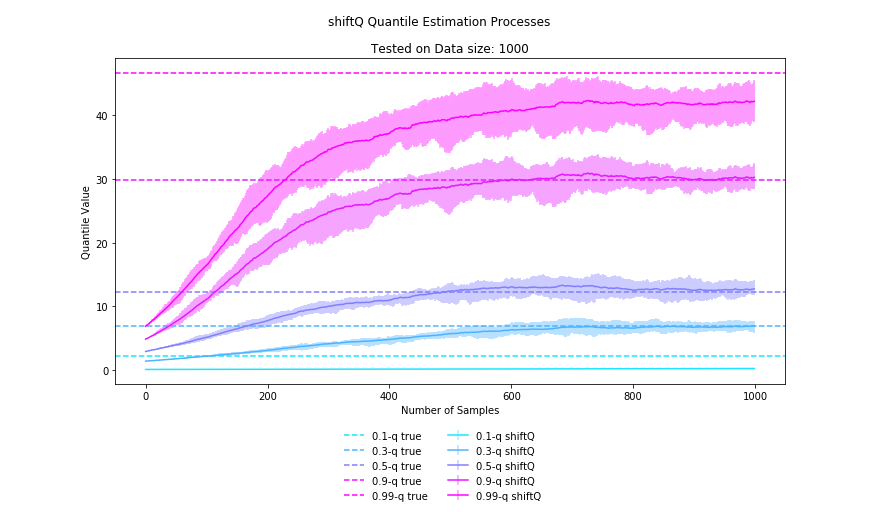
\includegraphics[width=1\columnwidth]{shiftQ/1000_proc.png}
	\caption{The shiftQ algorithm for Positive Gaussian 1 distribution (the process graph)}
    \label{fig: shiftQ_proc}
\end{figure}

\begin{figure}[h!]
	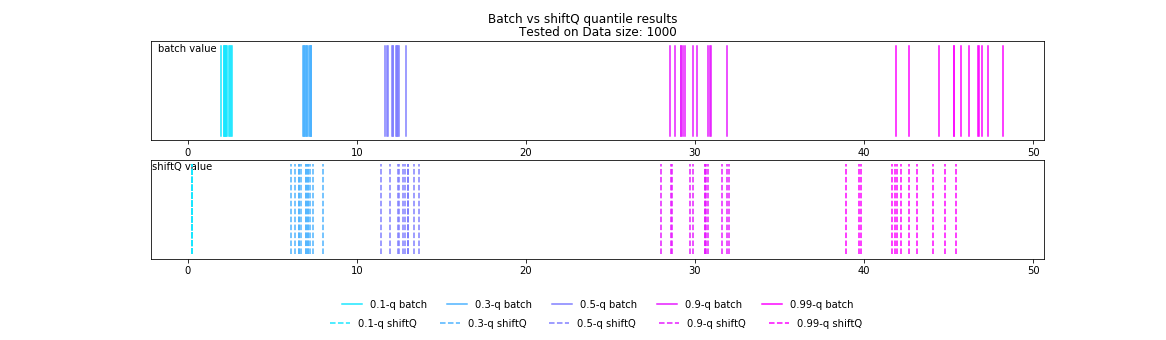
\includegraphics[width=1\columnwidth]{shiftQ/1000_res.png}
	\caption{The shiftQ algorithm for Positive Gaussian 1 distribution (the result graph)}
    \label{fig: shiftQ_res}
\end{figure}

\begin{figure}[h!]
	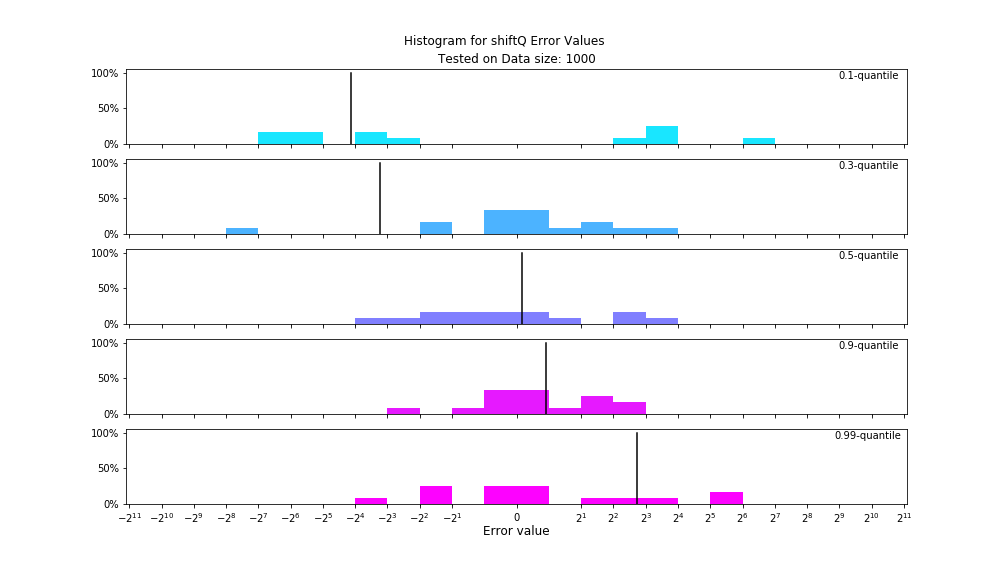
\includegraphics[width=1\columnwidth]{shiftQ/1000_err.png}
	\caption{The shiftQ algorithm for Positive Gaussian 1 distribution (the error graph)}
    \label{fig: shiftQ_err}
\end{figure}

\begin{figure}[h!]
	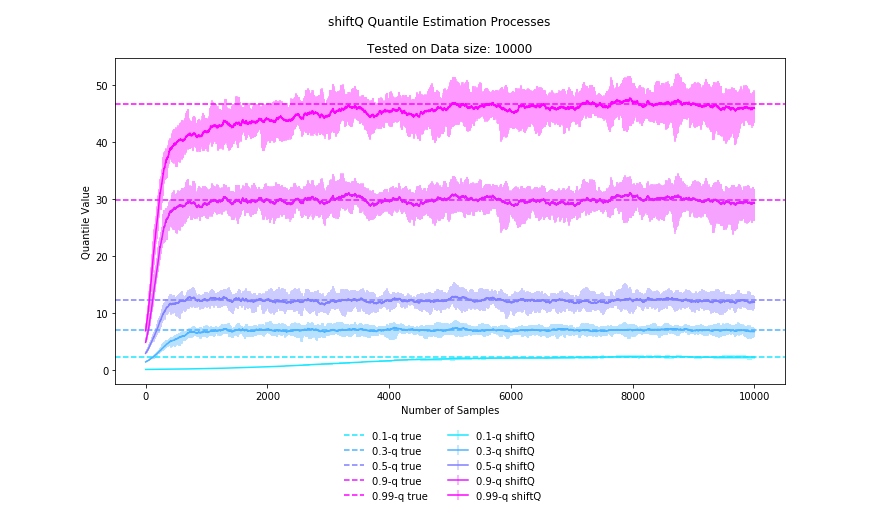
\includegraphics[width=1\columnwidth]{shiftQ/10000_proc.png}
	\caption{The shiftQ algorithm for Positive Gaussian 1 distribution (the process graph)}
    \label{fig: shiftQ_proc_10000}
\end{figure}

 In the process plot in Fig \ref{fig: shiftQ_proc} the quantile estimates for $0.1$-q and $0.99$-q have not converged even after 1000 epochs. From the comparison with the 0.5-q we can see that this big error is not caused by the initialization value of 0.1-q. Specifically, the shiftQ 0.5-q converges even though the true quantile of it is further away from its initialization. Instead, the estimation of 0.1-q has barely changed during the 1000 epochs. The converging trend of 0.99-q is also too slow to reach the true 0.99-q quantile within 1000 epochs. The distance between the batch quantiles and shiftQ estimated quantiles in Fig \ref{fig: shiftQ_res} has shown that the quantile estimates at both ends are far away from the batch quantiles. It is shown in the Fig \ref{fig: shiftQ_err} that the shiftQ algorithm has a largely varied performance on different quantiles. For example, the 0.5 and 0.9 quantiles has a much smaller and stable error distribution around 0, while the 0.1 quantile has a wide range of error values from less than -100 to more than 50. 
 
 To test the convergence of end quantile values, a further experiment is done with a dataset of 10000 samples. Fig \ref{fig: shiftQ_proc_10000} shows that both 0.1-q and 0.99-q estimates finally converge when there are a sufficient amount of samples.
% ----------------------------------- Extended P2 ---------------------------------------
\pagebreak
\section{The Extended $P^2$ Algorithm}
\label{sec: multi_{p2}}

The \textit{Extended $P^2$} algorithm\cite{raatikainenSequentialProcedureSimultaneous1993} uses exactly the same idea as the $P^2$ algorithm\cite{jainP2AlgorithmDynamic1985}. So for a better understanding, we introduce the $P^2$ algorithm first in \ref{subsubsec: description_{p2}}, then the generation method for the extended $P^2$ algorithm.
In section \ref{subsec: algo_extended_{p2}}, the detailed algorithm for extended $P^2$ is provided, followed by its experiment results in section \ref{subsec: exp_extended_{p2}}.

\subsection{Method Description}
\subsubsection{The $P^2$ Method}
\label{subsubsec: description_{p2}}

The intuition of the $P^2$ method is the assumption that any three adjacent quantiles form a parabolic formula.
Specifically, the method interprets quantile estimation as a relationship based on quantile values and their ordering positions, and applies either linear or parabolic adjustments based on the information from their neighbours.

Consider the straightforward quantile computation for [$\tau_1, ..., \tau_K$] that sorts all observations from the dataset $X = \{x_i\}^N_1$. Let $x_i$ denote the $i$th smallest value of $X$, then we have $x_1 < x_2 < ... < x_N$. 
To find the $\tau_i$-quantile of $X$, we need to find the data observation at \textit{marker position} $m_i = \tau_i (N-1) + 1$. Given the marker position, we then retrieve the value of the marker, the corresponding \textit{quantile value} $q_i = x_{m_i}$. 
For 3 adjacent quantiles at $\tau_{i-1}, \tau_i, \tau_{i+1}$, their quantile values can be independently computed in the same way, as shown in Figure \ref{fig: {multi_relationship_p2}}.

\begin{figure}[h]
    \centering
	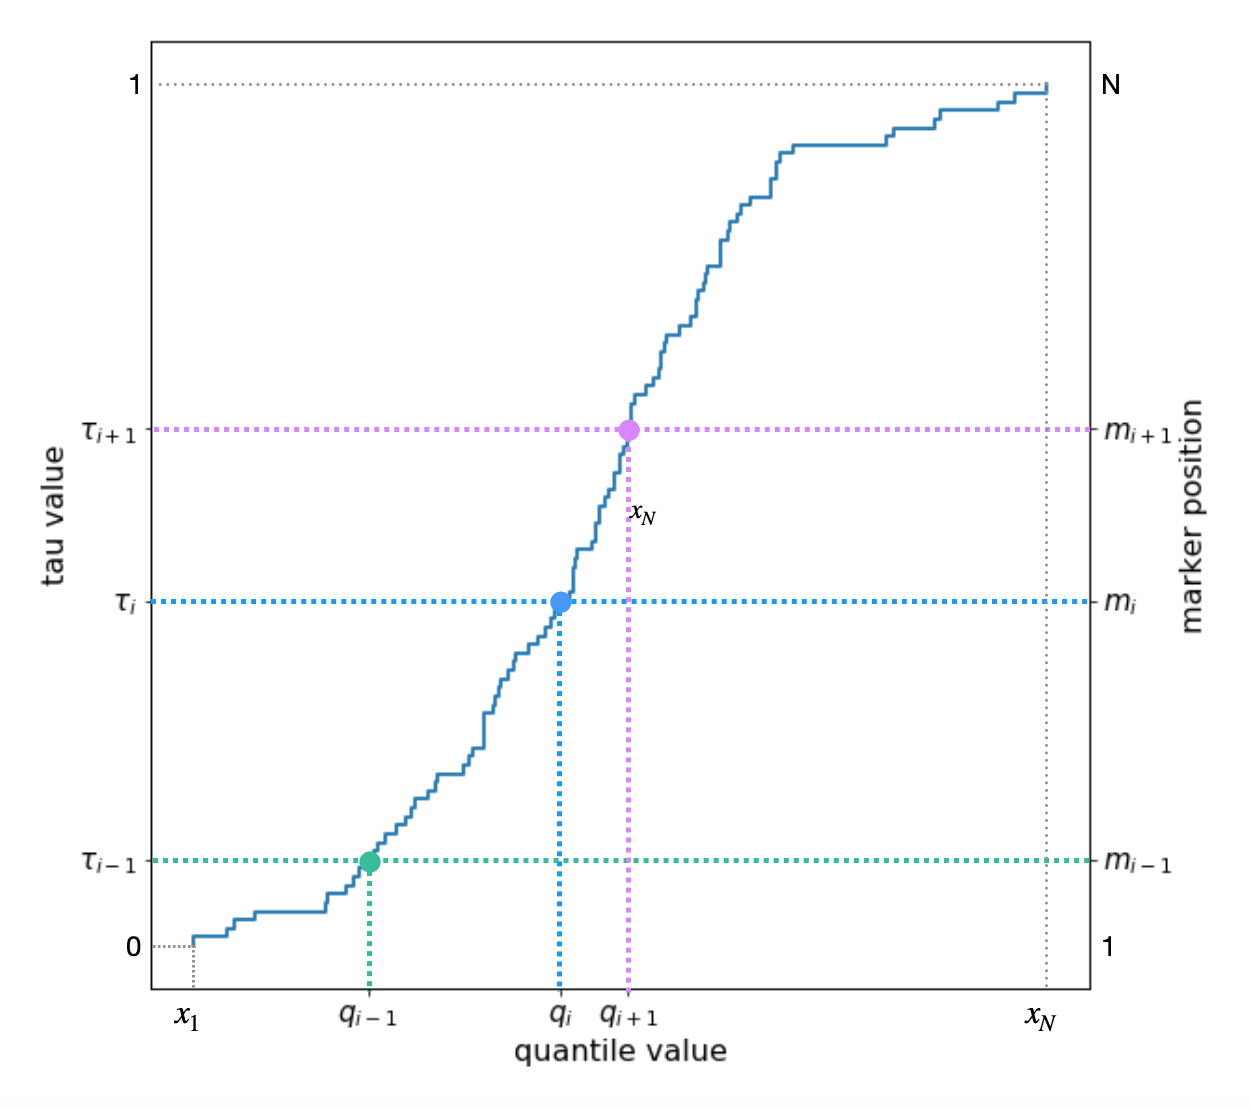
\includegraphics[width=0.8\columnwidth]{P2/relationships.png}
    \caption{Relationship between $\tau$ value, marker position and quantile values correspondingly for 3 adjacent quantiles}
    \label{fig: {multi_relationship_p2}}
\end{figure}

For quantile estimation, however, storing and sorting the entire dataset is infeasible. The $P^2$ method records only information only about the Target quantile values, and update them on the arrival of new observations. The update method, based on different conditions, is either a \textit{Piecewise-Parabolic} ($P^2$) formula, or a linear formula.

The information recorded for the $i$th quantile contains 3 parts: the marker position $m_i$, the desired marker position $m_i^\prime$, and the quantile value $q_i$. For quantile $\tau_i$ with current observation number $N$, the desired marker position is $m_i^\prime = 1 + (N-1)\tau$. This algorithm aims to keep each marker position $m_i$ close to its desired position $m_i^\prime$ as new observation come in. As $m_i$ is updated, $q_i$ is updated to an estimate of the new value of the $m_i$th data point.
% The quantile value estimation $q_i$ is then updated accordingly after the current marker position is fixed.
Figure \ref{fig: {multi_parabolic_p2}} demonstrates the update of $m_i$ and $q_i$.

\begin{figure}[h]
    \centering
	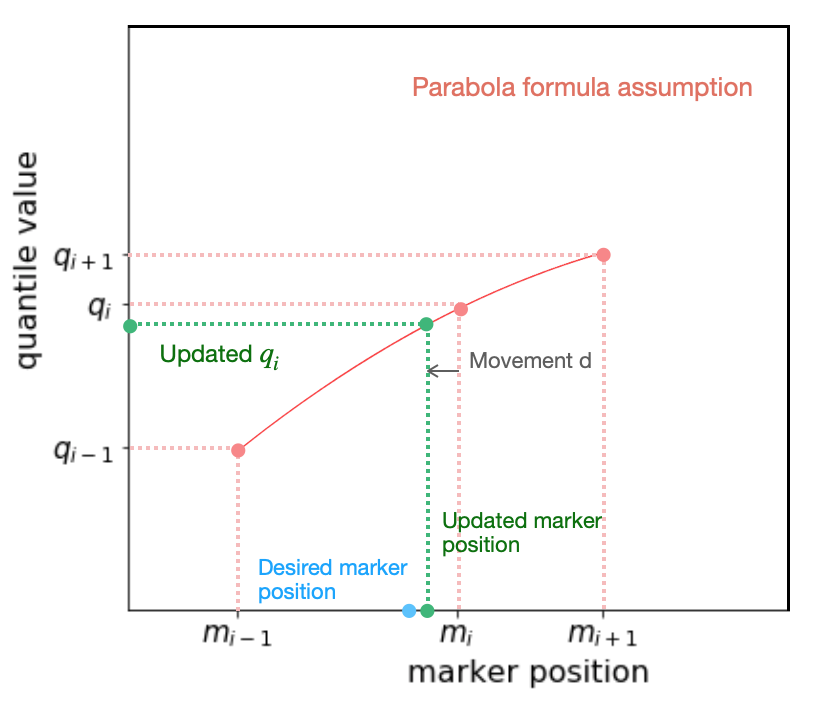
\includegraphics[width=0.7\columnwidth]{P2/parabola.png}
    \caption{Quantile value update using the Piecewise-Parabolic($P^2$) formula}
    \label{fig: {multi_parabolic_p2}}
\end{figure}

The quantile value update is based on the Piecewise-Parabolic assumption that any three adjacent makers form a parabolic curve of the form $q_i = aq_i^2 + bq_i + c$.

If a marker is moved $d$ positions to the right, the new quantile value is updated by the \textit{parabolic formula}:
\begin{align}
\begin{split}
    q_{i} \leftarrow q_{i}+ & \frac{d}{m_{i+1}-m_{i-1}}\\
    \cdot & { \bigg[ 
        \left(m_{i}-m_{i-1}+d\right) \frac{\left(q_{i+1}-q_{i}\right)}{\left(m_{i+1}-m_{i}\right)}
        +\left(m_{i+1}-m_{i}-d\right) \frac{\left(q_{i}-q_{i-1}\right)}{\left(m_{i}-m_{i-1}\right)}
        } \bigg] \\
    m_{i} \leftarrow m_{i}+&d \text{ where } d = \pm 1
\end{split}
\end{align}

When applying the parabolic update would violate the monotone property, the alternative update is a \textit{piecewise-linear formula}:
\begin{equation}
    \begin{array}{l}
    q_{i}=q_{i}+d \frac{\left(q_{i+d}-q_{i}\right)}{m_{i+d}-m_{i}} \\
    m_{i}=m_{i}+d
    \end{array}
\end{equation}

In short, the update method for $\tau_i$-quantile takes only 2 steps:\\
Before starting, the $P^2$ algorithm extends the set of target quantiles $\tau_1 <... < \tau_K$ with $0$ and $1$, giving the target quantiles $[0, \tau_1, ..., \tau_K, 1]$.
When a new observation comes,
\begin{enumerate}
    \item Update every marker position $m_i$ to approach the desired marker position $m_i^\prime$.
    \begin{enumerate}
        \item If the quantile value is bigger than the coming observation, move the marker position by one position to the right.
        \item Adjust the marker position again if it is more than one position away from the desired marker. The move $d$ is $1$ if the marker position moves right, and $-1$ for moving left.
    \end{enumerate}
    \item Update the quantile value
    \begin{enumerate}
        \item Try applying the parabolic update to the quantile value. Note it might change the increasing order of quantiles, that is, $q_{i+1} > q_{i}$.
        \item If the ordering of quantile values is changed by the parabolic update, try the linear update instead.
    \end{enumerate}
\end{enumerate}


\subsubsection{The Extended $P^2$ Method}
In $P^2$, the update of a quantile relies on its position relative to the neighbour markers, indicating the accuracy of neighbour marker positions is important. 
It sets one marker for each quantile value, that is, a total of $K$ markers for [$\tau_1, ..., \tau_K$].
The extended $P^2$ algorithm improves the estimation accuracy by the introduction of "middle markers",  which nearly doubles the amount of markers in $P^2$. 
This means, in the initialization part, there will be $2K+3$ markers for
$$
\tau = 0, \frac{0+\tau_1}{2}, \tau_1, \frac{\tau_1 + \tau_2}{2}, \tau_2, ..., \tau_{K}, \frac{\tau_K+1}{2}, 1
$$
And the estimation update for all those markers follows the same rule as in the $P^2$ algorithm.

The only difference between extended $P^2$ and $P^2$ is the extension of markers at the initialization stage. At a doubly expensive computation cost, the quantile estimation reaches a higher accuracy from the extra information, as shown in the work of \citeauthor{raatikainenSequentialProcedureSimultaneous1993}\cite{raatikainenSequentialProcedureSimultaneous1993}. Besides the extra information brought by the extra markers, the extended $P^2$ algorithm also benefits from a better initialization by a larger sampling. The larger sampling in extended $P^2$ reduces the possibility of severely unevenly distributed initializations, which becomes important for  $P^2$, as it is sensitive to the initialization of quantiles.
% In $p^2$, only desired quantiles have their information recorded and used for 

% \subsection{The Algorithm of Extended $P^2$}
% \label{subsec: algo_extended_{p2}}
Pseudocode for the $P^2$ algorithm is presented in algorithm \ref{alg:multi_p2} followed by the extended $P^2$ algorithm in algorithm \ref{alg:multi_ext_p2}.
\begin{algorithm}
    \caption{The $P^2$ Algorithm}\label{alg:multi_p2}
        \begin{algorithmic}[1]
            \Require{Dataset $X$, $K$ target quantile values $[\tau_1, \tau_2, ..., \tau_K]$}
            \Ensure{Targe quantile estimates $[\tau_1\text{-}q, \tau_2\text{-}q, ..., \tau_K\text{-}q]$}
            \State
            \State {\textbf{0.Extend number of markers from $K$ to $K' = K+2$}}
            \LineComment{Add $0$ and $1$ before and after the target quantiles.}
            \State{$[\tau_1^\prime, \tau_2^\prime, ..., \tau_{K'}^\prime] = [0, \tau_1, \tau_2, ..., \tau_{K}, 1]$}
            \State
            \State{\textbf{A. Initialization}}
            \State {The first $K'$ observations (sorted): \{$x_1,x_2,...,x_{K'}$\}}
            \For{$(i = 1, ..., K')$}
                \State {Marker height:    $q_i = x_i $}
                \State {Marker position:   $m_i = i$}
                \State {Desired Marker position:  $m_i^\prime = ((K')-1)\tau_i + 1$}
            \EndFor

            \State
            \State{\textbf{B. For each new observation $x_j$, $j \geq K'+1$, perform the following}}
            \Switch{$s$}            \Comment {Find the cell $k$ such that $q_k \leq x_j < q_{k+1}$}
                \Case{$x_j < q_1$}
                    \State{$q_1 = x_j, k = 1$}
                \EndCase
                \Case{$q_i \leq x_j < q_{i+1}$}
                    \State {$k = i$}
                \EndCase
                \Case{$q_K < x_j$}
                    \State {$q_K = x_j, k = K'-1$}
                \EndCase
            \EndSwitch
            \State
            
            \State{$m_i = m_i + 1$; $i = k+1, ..., K'$}       \Comment{Increment markers above new observation}
            % \Comment{Different from that on the $P^2$ paper}
            \State{$m_i^\prime = m_i^\prime + \tau_i'$; $i = 1, ..., K'$}            \Comment{Update all the desired positions}

            \State
            \State{Adjust marker heights $2$ to $K'-1$ if necessary:}
            \For{$i = 2, 3, ..., K-1$}
                \State {$d_i = m_i^\prime - m_i$}
                \If {($ d_i \geq 1 \text{ and }  m_{i+1} - m_i > 1$) or 
                     ($ d_i \leq -1 \text{ and }  m_{i-1} - m_i < -1$) }
                    \State {$d_i = sign(d_i)$}
                    \State {$q_i^\prime = \text{parabolic}(q_i)$}     \Comment{Try the $P^2$ update}
                    \If {$ q_{i-1} < q_i^\prime < q_{i+1}$}
                        \State {$q_i = q_i^\prime$}
                        \Else                           \Comment{Else use linear update}
                            \State{$q_i = \text{linear}(q_i)$}
                    \EndIf
                    \State {$m_i = m_i + d_i$}          \Comment{Update marker position}
                \EndIf
            \EndFor

            \State
            \State {\textbf{C. Return quantile estimates} }     
            \LineComment{The result is available after any number of observations}
            \State {$[\tau_1\text{-}q, \tau_2\text{-}q, ..., \tau_K\text{-}q] = [q_2, q_2, ..., q_{K+1}]$}
        \end{algorithmic}
\end{algorithm}
\\\\
The extended $P^2$ extends the number of quantile markers of the $P^2$ algorithm at the initialization step, then follows $P^2$ in the next steps.

\begin{algorithm}
    \caption{Extended $P^2$ Algorithm}\label{alg:multi_ext_p2}
        \begin{algorithmic}[1]
            \Require{Dataset $X$, Demanding quantile values $[\tau_1, \tau_2, ..., \tau_K]$}
            \Ensure{Demaning quantile estimates $[\tau_1\text{-}q, \tau_2\text{-}q, ..., \tau_K\text{-}q]$}

            \State
            \State {\textbf{0.Extend number of markers from $K$ to $2K+3$}}
            \LineComment{Evenly fill the intervals between $0,1$ and each 2 quantile values}
            \State{$[\tau_1^\prime, \tau_2^\prime, ..., \tau_{2K+3} ^\prime] = [0, \frac{0+\tau_1}{2}, \tau_1, \frac{\tau_1 + \tau_2}{2}, \tau_2, ..., \tau_{K}, \frac{\tau_K+1}{2}, 1]$}

            \State
            \State{\textbf{1. Apply $P^2$ with the extended initialization}}
            \LineComment{And returns an estimate of extended list}
            \State{$[q_1^\prime, ..., q_{2K+3}^\prime] = P^2$ ($X$, $[\tau_1^\prime, \tau_2^\prime, ..., \tau_{2K+3} ^\prime]$)}
            \State
            \State {\textbf{2. Return quantile estimates} } 
            \State {Extract the quantile estimates for the original $M$ quantile values}
            \State {$[\tau_1\text{-}q, \tau_2\text{-}q, ..., \tau_K\text{-}q] = [q_3^\prime, q_5^\prime, ..., q_{2K+1}^\prime]$}
        \end{algorithmic}
\end{algorithm}

% 0, 0.5, 1, 1.5, 2, ..., M,    (M+1)/2, 1
% 1, 2,   3, 4,   5, ..., 2M+1, 2M+2,   2K+3            

\subsection{Experiment Results}
\label{subsec: exp_extended_{p2}}
The $P^2$ algorithm is tested on the Gaussian 1 distribution on 1000 samples.The process plot Fig \ref{fig: p2_proc} shows the convergence of different quantiles have slightly different pace, in that the 0.9 and 0.99 are very close to the true quantile value while the other 3 have already stayed stable at the 1000th epoch. Fig \ref{fig: p2_res} shows the final results are close, which is evaluated in Fig \ref{fig: p2_err} that error values of extended $p^2$ estimates has limited error values between -20 and 10 for all quantiles except for one outlier at -80. 
Overall the extended $P^2$ method has a really fast convergence rate.

\begin{figure}[h!]
	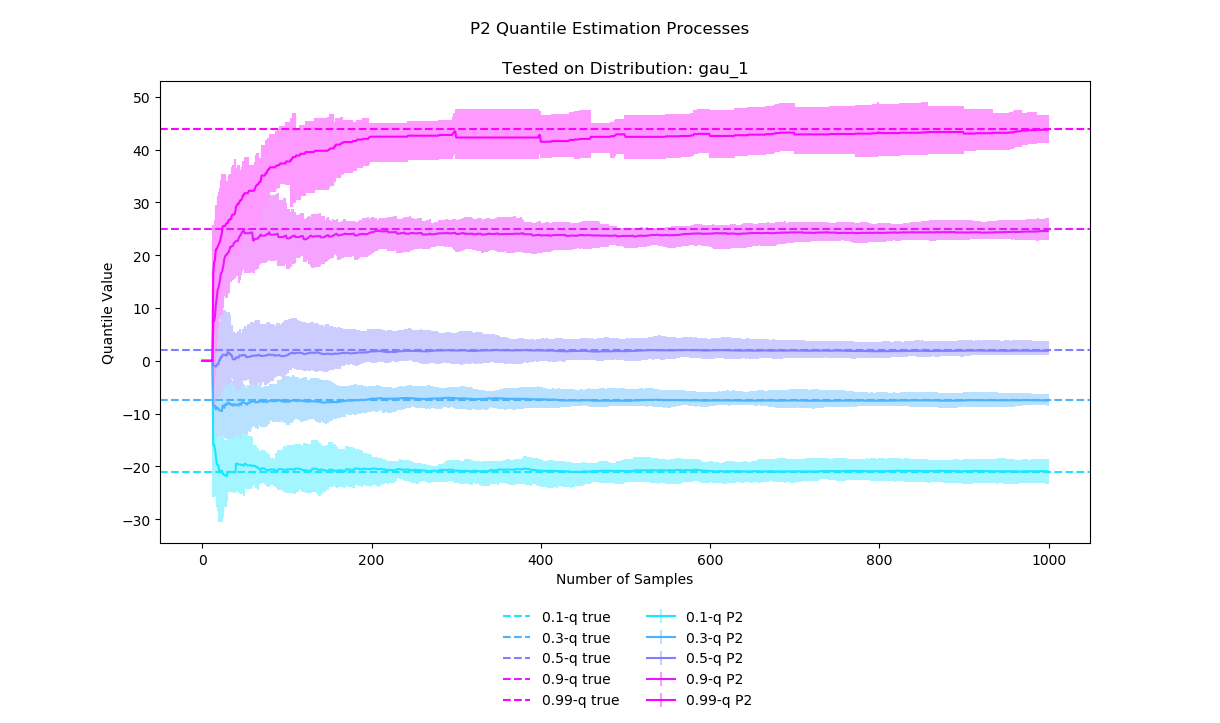
\includegraphics[width=1\columnwidth]{P2/gau_1_proc.png}
    \caption{The extended $P^2$ algorithm for Gaussian 1 distribution (the process graph)}
    \label{fig: p2_proc}
\end{figure}

\begin{figure}[h!]
	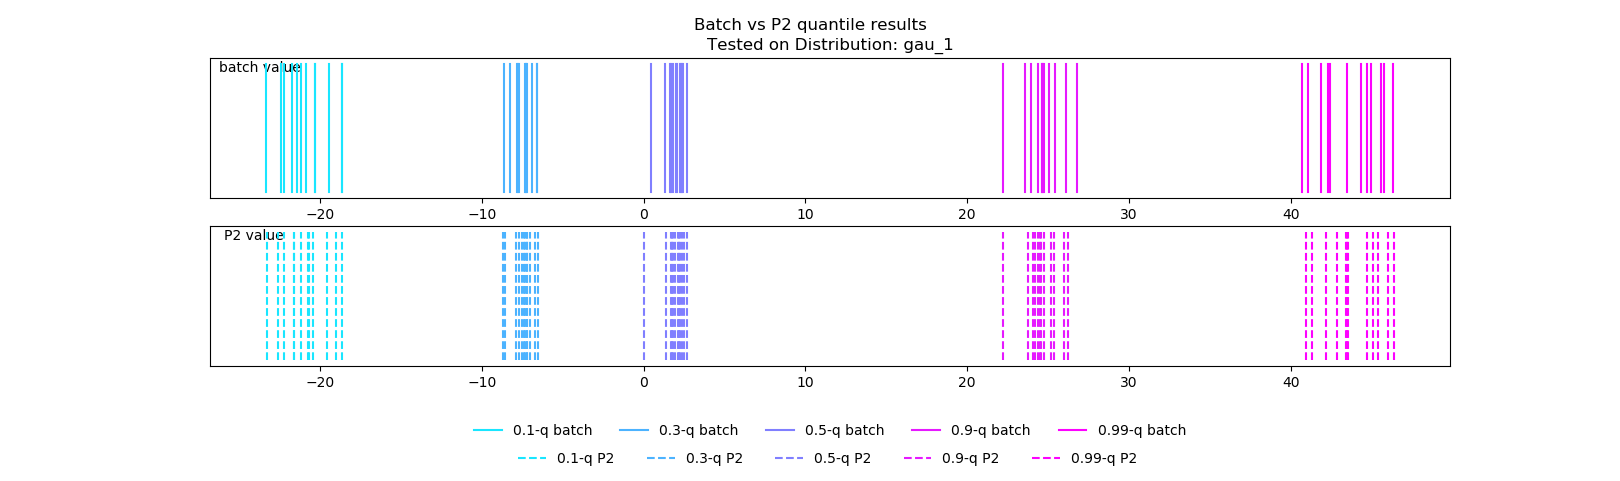
\includegraphics[width=1\columnwidth]{P2/gau_1_res.png}
	\caption{The extended $P^2$ algorithm for Gaussian 1 distribution (the result graph)}
    \label{fig: p2_res}
\end{figure}

\begin{figure}[h!]
	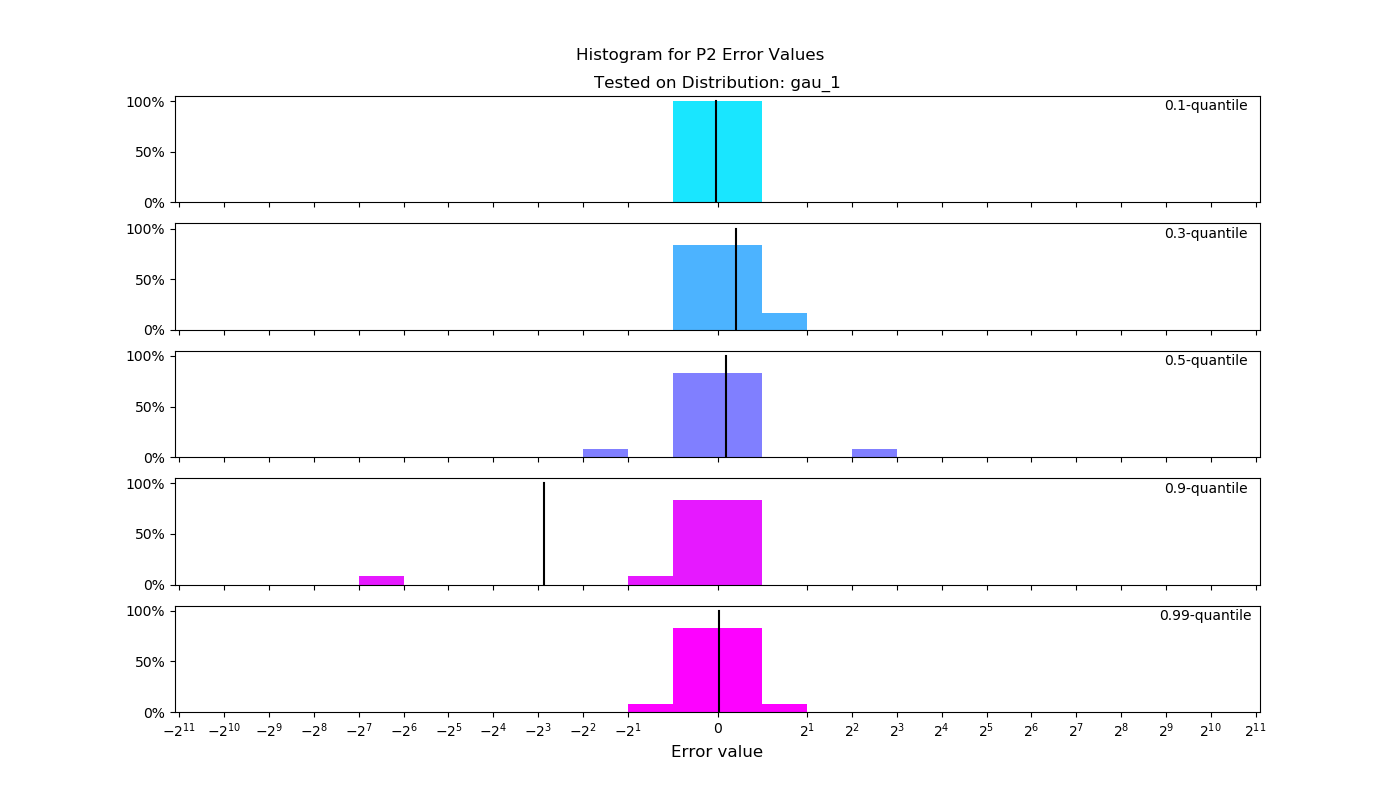
\includegraphics[width=1\columnwidth]{P2/gau_1_err.png}
    \caption{The extended $P^2$ algorithm for Gaussian 1 distribution (the error graph)}
    \label{fig: p2_err}
\end{figure}

\marginline{this will be edited later}
\section{Conclusion}
\label{sec: multi_discussion}

From the experimental results we can see the two multi-quantile estimation methods can solve the crossing problem by introducing some mathematical relationship assumptions between adjacent quantiles. The following step will be doing nothing but to 


\cleardoublepage % Empty page before the start of the next part

%------------------------------------------------
% part 2

% \ctparttext{You can put some informational part preamble text here. Illo principalmente su nos. Non message \emph{occidental} angloromanic da. Debitas effortio simplificate sia se, auxiliar summarios da que, se avantiate publicationes via. Pan in terra summarios, capital interlingua se que. Al via multo esser specimen, campo responder que da. Le usate medical addresses pro, europa origine sanctificate nos se.} % Text on the Part 2 page describing the content in Part 2

% \cleardoublepage % Empty page before the start of the next part
% \appendix
% \part{Appendix} % New part of the thesis for the appendix

%----------------------------------------------------------------------------------------
%	THESIS CONTENT - APPENDICES
%----------------------------------------------------------------------------------------

% \include{Chapters/Chapter0A} % Appendix A
%\include{Chapters/Chapter0B} % Appendix B - empty template

%----------------------------------------------------------------------------------------
%	POST-CONTENT THESIS PAGES
%----------------------------------------------------------------------------------------

\cleardoublepage% Bibliography

\label{app:bibliography} % Reference the bibliography elsewhere with \autoref{app:bibliography}

\manualmark % Work-around to have small caps also here in the headline
\markboth{\spacedlowsmallcaps{\bibname}}{\spacedlowsmallcaps{\bibname}} % Work-around to have small caps also
%\phantomsection
\refstepcounter{dummy}

\addtocontents{toc}{\protect\vspace{\beforebibskip}} % Place the bibliography slightly below the rest of the document content in the table of contents
\addcontentsline{toc}{chapter}{\tocEntry{\bibname}}

\printbibliography % Bibliography

% \cleardoublepage% Declaration

\refstepcounter{dummy}
\pdfbookmark[0]{Declaration}{declaration} % Bookmark name visible in a PDF viewer

\chapter*{Declaration} % Declaration section text

\thispagestyle{empty}

Put your declaration here.
\bigskip
 
\noindent\textit{\myLocation, \myTime}

\smallskip

\begin{flushright}
\begin{tabular}{m{5cm}}
\\ \hline
\centering\myName \\
\end{tabular}
\end{flushright}
 % Declaration


%----------------------------------------------------------------------------------------

\end{document}
